\documentclass[11pt,oneside]{uhthesis}
\usepackage{mathpazo}

\renewcommand{\tablename}{Tabla}
\title{Una propuesta para encontrar el sistema de ecuaciones diferenciales lineales en los parámetros que mejor ajuste un conjunto de datos}
\author{Enrique Martínez González}
\advisor{MSc. Fernando Rodríguez Flores}
\coadvisor{Lic. Ernesto Borrego Rodríguez}
\degree{Licenciado en Ciencias de la Computación}
\faculty{Facultad de Matemática y Computación}
\date{Diciembre de 2022}
\logo{Graphics/uhlogo}


\begin{document}
\selectlanguage{spanish}

\frontmatter
\maketitle

\begin{dedication}
    \textit{
        Hola que tal\\
        si, aquí va la dedicatoria y tal}
\end{dedication}
\chapter*{Agradecimientos}\label{chapter:agradecimientos}

A mi tutor Fernando Rodríguez, por dedicar su valisísimo tiempo y geniales ideas a la realización de este trabajo. Por guiarme durante todo este proceso y regalarme sus conocimientos y consejos.
\\

A Ernesto Borrego por aconsejarme tan fabuloso tutor y por su preocupación constante acerca del avance de la investigación.
\\

A David Guaty por su apoyo y gran habilidad en la solución de problemas matemáticos.
\\

A mi hermano Fernando en su enseñanza de buenas prácticas en la programación.
\\

A mi madre Elizabeth por su amor y dedicación en este trabajo.
\\

A Dianelys por acogerme como otro hijo durante esta etapa.
\\

A Diana por su apoyo incondicional.
\\

Al resto de mi familia por siempre estar presentes en mi vida apoyándome a seguir adelante.

\begin{opinion}
    Y aqui va la opinión del tutor :D

    \vspace{1cm}


    \begin{flushright}
        \underline{\hspace{6.5cm}}\\
        MSc. Fernando Raul Rodriguez Flores

        Facultad de Matemática y Computación

        Universidad de la Habana

        Noviembre, 2022
    \end{flushright}

\end{opinion}
\begin{abstract}

    Los sistemas de ecuaciones diferenciales ordinarias lineales con respecto a los parámetros se pueden utilizar para predecir y describir fenómenos de la naturaleza, la ciencia, la tecnología y la sociedad. Esta predicción se realiza mediante la generación de modelos matemáticos a partir de observaciones del fenómeno. La obtención del modelo permite analizar la relación entre las distintas variables y parámetros que ocurren en el fenómeno observado.

    Para encontrar de forma automática modelos que desriben un conjunto de datos se desarrollan diversos métodos que son capaces de plantear de forma simbólica los sistemas que describen los datos. Estos algoritmos utilizan el método de regresión simbólica. La problema de regresión simbólica en sistemas de ecuaciones diferenciales se puede resolver mediante el uso de algoritmos genéticos o redes neuronales.

    En este trabajo se propone una herramienta para encontrar el sistema de ecuaciones diferenciales lineales con respecto a los parámetros que mejor describa un conjunto de datos utlizando regresión simbólica mediante algoritmos genéticos. Se aproximan los parámetros presentes en el modelo mediante la solución de un sistema de ecuaciones lineales y en caso de que los datos presenten ruido se utiliza un spline de suavizado para la aproximación de los datos. El comportamiento de la herrmienta propuesta muestra la capacidad de generación de un sistema que describe los datos, incluso ante la presencia de ruido.


\end{abstract}

\begin{enabstract}

    Ordinary differential equations systems linear with respect to parameters can be used to predict and describe phenomena in nature, science, technology, and society. This prediction is made by generating mathematical models from observations of the phenomenon. Obtaining the model allows to analyze the relationship between the different variables and parameters that occur in the observed phenomenon.

    To automatically find models that describe a set of data, various methods are developed that are capable of symbolically posing the systems that describe the data. These algorithms use the symbolic regression method. The symbolic regression problem in systems of differential equations can be solved by using genetic algorithms or neural networks.

    In this work, a tool is proposed to find the oridnary differential equations system linear with respect to the parameters that best describes a data set using symbolic regression through genetic algorithms. The parameters present in the model are approximated by solving a linear equations system and in case the data present noise, a smoothing spline is used to approximate the data. The behavior of the proposed tool shows the generation capacity of a system that describes the data, even in the presence of noise.

\end{enabstract}
\tableofcontents
\listoffigures

\mainmatter

\chapter*{Introducción}\label{chapter:introduction}
\addcontentsline{toc}{chapter}{Introducción}

\qquad

La regresión es un conjunto de procesos estadísticos para estimar las relaciones entre una variable dependiente y una o más variables independientes. La forma más común de análisis de regresión es la regresión lineal, en la que se encuentra la línea o una combinación lineal más compleja que se ajusta más a los datos de acuerdo con un criterio matemático específico. Por ejemplo, el método de los mínimos cuadrados ordinarios calcula el único hiperplano que minimiza la suma de las diferencias al cuadrado entre los datos dados y ese hiperplano. Por razones matemáticas específicas, esto le permite al investigador estimar la variable dependiente cuando las variables independientes toman un conjunto dado de valores.

El análisis de regresión se utiliza principalmente para dos propósitos conceptualmente distintos.

\begin{itemize}
    \item Primero, el análisis de regresión se usa ampliamente para la predicción y el pronóstico de datos.
    \item En segundo lugar, en algunas situaciones se puede utilizar el análisis de regresión para inferir relaciones causales entre las variables independientes y dependientes.
\end{itemize}

La primera forma de regresión fue el método de mínimos cuadrados, que fue publicado por Legendre en 1805, y por Gauss en 1809. Legendre y Gauss aplicaron el método al problema de determinar, a partir de observaciones astronómicas, las órbitas de los cuerpos alrededor del Sol, en su mayoría cometas, pero también más tarde los planetas menores recién descubiertos.

En las décadas de 1950 y 1960, los economistas utilizaron "calculadoras" de escritorio electromecánicas para calcular las regresiones. Antes de 1970, a veces tomaba hasta 24 horas recibir el resultado de una regresión.

Los métodos de regresión continúan siendo un área de investigación activa. En las últimas décadas, se han desarrollado nuevos métodos para la regresión robusta, regresión que involucra respuestas correlacionadas como series de tiempo y curvas de crecimiento, regresión en la que el predictor o las variables de respuesta son curvas, imágenes, gráficos u otros objetos de datos complejos, métodos de regresión que acomodan varios tipos de datos faltantes, regresión no paramétrica, métodos bayesianos para la regresión, regresión en la que las variables predictoras se miden con error, regresión con más variables predictoras que observaciones e inferencia causal con regresión.

Si se tiene un conjunto de puntos de la forma $<t_i, y_i>$ y se desea determinar automáticamente el sistema de ecuaciones diferenciales ordinarias que mejor describe el conjunto de datos y que además, sea lineal en los parámetros, se pudiese utilizar regresión para resolver este problema.

A continuación se describirá brevemente qué significa que la ecuación diferencial sea lineal en los parámetros y que mejor describa los datos.

Que el sistema sea lineal en los parámetros significa que cada componente de la parte derecha de la ecuación diferencial es una función de la forma:

$$f_j(t,y) = \sum_{i=1}^{n} a_i * g_i(t, y)$$

donde los $a_i$ son parámetros y todas las funciones $g_i(t,y)$ son funciones que dependen de la variable $t$, de la variable $y$, pero no dependen de ningún parámetro.

Si se plantea que $y(t_i)$ es la solución de la ecuación diferencial evaluada en el punto $t_i$, entonces un indicador de cuán bien este sistema describe los datos pudiera ser el valor $L$, donde:

$$L = \sum_{i=1}^{n} (y(t_i) - y_i)^2$$

Cuando se usa un valor como $L$ en el que se considera la suma de cuadrados de las diferencias, se dice que estamos en presencia de un problema de mínimos cuadrados, porque lo que se quiere es minimizar esa suma de cuadrados.

Entonces, buscar el sistema de ecuaciones diferenciales que mejor describe los datos, se reduce a buscar el sistema de ecuaciones diferenciales que haga que el valor de $L$ sea lo más pequeño posible.

Al aplicar regresión se pudiese obtener el conjunto de curvas y predecir valores de esta en función de la investigación que se desee realizar.


\subsection*{Objetivos}

La investigación tiene como \textbf{objetivo general} la creación de una herramienta que permita encontrar de forma automática el sistema de ecuaciones diferenciales lineales en los parámetros que mejor ajuste un conjunto de datos dados. Para dar cumplimiento a la idea anterior se trazaron los siguientes objetivos específicos:


\subsubsection*{Objetivos específicos}

\begin{enumerate}
    \item Consultar literatura especializada sobre el estado del arte de los problemas de regresión en sistemas de ecuaciones, específicamente las propuestas existentes para encontrar sistemas que cumplan las características antes mencionadas.
    \item Investigar sobre las diferencias que plantea la regresión simbólica
    \item Estudiar acerca de metaheurísticas, específicamente los algoritmos genéticos.
    \item Crear un marco experimental que permita evaluar la calidad de la herramienta implementada ante distintos modelos de ecuaciones diferenciales
    \item Analizar los resultados obtenidos a través de un conjunto de métricas y técnicas de visualización.
\end{enumerate}

\subsection*{Organización de la tesis}

El presente documento está organizado en 4 capítulos que recogen las
distintas etapas por las que transitó la investigación.

En el capítulo 1 \textbf{Elementos de la regresión simbólica} se realiza una
introducción a los elementos y conceptos de esta área abordados a lo largo
del trabajo.

\chapter{Descripción del problema}\label{chapter:problemIntro}

Dado un conjunto de puntos de la forma $<ti, yi>$ se desea determinar automáticamente el sistema de ecuaciones diferenciales ordinarias que mejor describe el conjunto de datos y que además, sea lineal en los parámetros.

A continuación se describirá brevemente qué significa que la ecuación diferencial sea lineal en los parámetros y que mejor describa los datos.

\section{Función lineal con respecto a los parámetros}

Que el sistema sea lineal en los parámetros significa que cada componente de la parte derecha de la ecuación diferencial es una función de la forma:

$$f_j(t,y) = a1 * g1(t,y) + a2 * g2(t,y) + …  + an * gn(t,y)$$

donde los ai son parámetros y todas las funciones gi(t,y) son funciones que dependen de la variable t, de la variable y, pero no dependen de ningún parámetro.  Un ejemplo de sistema que cumple esta características es el sistema SIR:

$$S’ = - a*I*S$$
$$I’ = a*I*S - b*I$$
$$R’ = b*I$$

Este modelo indica la cantidad de individuos susceptibles, infectados y recuperados de una enfermedad en un instante de tiempo. En este caso, se tiene que la función

$$f_S (t,S,I,R) = a1 * g_s1 (t,S,I,R)$$

donde:

$$g_s1(t,S,I,R) = -I*S$$

La parte de derecha de la segunda ecuación (I’ = a\*I\*S - b*I) sería:

$$f_I (t,S,I,R) = b1 * g_I1 (t,S,I,R) + b2 * g_I2 (t,S,I,R)$$

donde:

$$g_I1(t,S,I,R) = I*S, y g_I2(t,S,I,R) = -I$$

La parte de derecha de la tercera ecuación $(R’ = b*I)$ sería:

$$f_R (t,S,I,R) = b1 * g_R1 (t,S,I,R)$$

donde:

$$g_R1(t,S,I,R) = I$$

En este caso, se cumple además, que algunos de los parámetros presentes en varias de las ecuaciones son los mismos, pero eso no es un requisito para que sea lineal con respecto a las parámetros.

Este sistema SIR se puede ver gráficamente como:

\begin{figure}[!h]
    \centering

    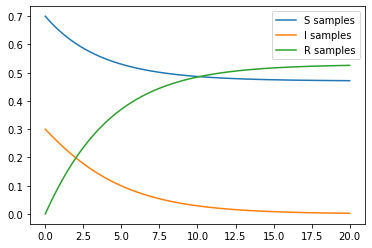
\includegraphics[width=3in]{Graphics/sir_model.png}

    \caption{ \small{Modelo de SIR.}}

    \label{sir_model}

\end{figure}

y este indica en una población con una enfermedad, como se va desplazando la cantidad de susceptibles, infectados y recuperados a lo largo del tiempo.

\section{Sistema de ecuaciones diferenciales que mejor describa los datos}

Dado un conjunto de puntos de la forma $<ti, yi>$ y un sistema de ecuaciones diferenciales $y’ = f(t,y)$, se puede tener un indicador de cuán bien ese sistema describe esos datos.

Si decimos que $y(ti)$ es la solución de la ecuación diferencial evaluada en el punto $ti$, entonces un indicador de cuán bien ese sistema describe los datos pudiera ser el valor $L$:

$$L = (y(t1) - y1)^2 + (y(t2) - y2)^2 + …  + (y(tn) - yn)^2$$

Esto es una suma de cuadrados, que se puede escribir con una sumatoria, aunque se expresa la versión explícita.

Cuando se usa un valor como L en el que se considera la suma de cuadrados de las diferencias, se dice que estamos en presencia de un problema de mínimos cuadrados, porque lo que se quiere es minimizar esa suma de cuadrados.

Entonces, buscar el sistema de ecuaciones diferenciales que mejor describe los datos, se reduce a buscar el sistema de ecuaciones diferenciales que haga que el valor de L (la suma de cuadrados) sea lo más pequeño posible.

Pero, aquí no interesa cualquier sistema de ecuaciones diferenciales: interesa los que sean lineales con respecto a los parámetros

Este sistema de ecuaciones diferenciales deseado se vería gráficamente como un sistema que solapa al original:

\begin{figure}[!h]
    \centering

    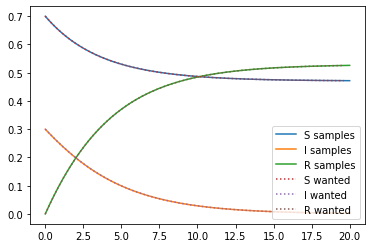
\includegraphics[width=3in]{Graphics/sir_model_wanted.png}

    \caption{ \small{Modelo de SIR original y modelo de SIR que se desea encontrar.}}

    \label{sir_model_wanted}

\end{figure}
\chapter{Propuesta de solución}\label{chapter:SolutionProposal}

En la sección anterior definimos los términos necesarios para entender el problema que consiste en:

Dado un conjunto de puntos de la forma $<ti,yi>$ encontrar un sistema de ecuaciones diferenciales que mejor describa los datos (en el sentido de los mínimos cuadrados).

En esta sección se tratarán varios elementos: regresión simbólica y de algoritmos genéticos.  Para usar un algoritmo genético es necesario definir cuáles son las posibles soluciones y para esas soluciones definir en qué consiste el cruzamiento, la mutación y cómo se puede saber cuán buena es una solución dada.

\section{Regresión simbólica}

La regresión simbólica que es un tipo de regresión que busca dentro de un espacio de expresiones matemáticas el modelo que mejor se ajuste a un conjunto de datos dados. En esta ningún modelo en particular es utilizado en el comienzo, en su lugar se generan expresiones que se forman de manera aleatoria combinando operaciones matemáticas, funciones analíticas, constantes y variables. Normalmente la regresión simbólica para funciones matemáticas es atacado con una variedad de métodos, uno de ellos es la recombinación de ecuaciones usando algoritmos evolutivos y uno de estos puede ser un algoritmo genético.

Al no requerir una especificación a priori de un modelo, la regresión simbólica no se ve afectada por el sesgo humano o las brechas desconocidas en el conocimiento del dominio. Intenta descubrir las relaciones intrínsecas del conjunto de datos, al permitir que los patrones en los propios datos revelen los modelos apropiados, en lugar de imponer una estructura de modelo que se considere matemáticamente manejable desde una perspectiva humana. La función de ajuste que impulsa la evolución de los modelos tiene en cuenta no solo las métricas de error (para garantizar que los modelos predigan los datos con precisión), sino también medidas especiales de complejidad, lo que garantiza que los modelos resultantes revelen la estructura subyacente de los datos en un manera que sea comprensible desde una perspectiva humana. Esto facilita el razonamiento y favorece las probabilidades de obtener información sobre el sistema de generación de datos.

Se ha demostrado que la regresión simbólica es un problema NP-difícil, en el sentido de que no siempre se puede encontrar la mejor expresión matemática posible para ajustarse a un conjunto de datos dado en tiempo polinomial.

\section{Algoritmos genéticos}

En ciencias de la computación un algoritmo genético es una metaheurística inspirada en el proceso natural de selección. Estos usualmente son utilizados para generar soluciones de alta calidad en problemas de optimización y búsqueda haciendo uso de los conocimientos de la biología, utilizando las acciones de mutación, cruzamiento y selección para modificar una población de individuos con el objetivo de obtener la solución deseada.

Para usar un algoritmo genético es necesario definir varios elementos:

- Cuáles son las posibles soluciones
- Cómo aplicar un operador de cruzamiento
- Cómo aplicar un operador de mutación
- Cómo determinar cuán buena es una solución
- Cómo determinar qué soluciones pasan a las próximas generaciones

Nuestro problema consiste en determinar el sistema de ecuaciones diferenciales que mejor se ajuste a un conjunto de datos y que sean lineales en los parámetros.

Con esto en mente, nuestras soluciones serían los posibles sistemas de ecuaciones lineales que cumplan con esas características. Por eso, en las próximas secciones vamos a describir: cómo representar las soluciones, cómo hacer cruzamientos y mutaciones, y cómo determinar cuán buena es una solución.

\section{Cómo representar una solución}

Como queremos resolver el problema de regresión simbólica en EDOs lineales en los parámetros, eso significa que estamos buscando una ecuación diferencial (lineal en los parámetros) que mejor ajuste los datos. Para ello, lo primero es decidir cómo representar los posibles sistemas.

Una vez que tengamos los datos $<ti, yi>$, tenemos algunas informaciones relevantes. Por ejemplo, si cada elemento de los datos es de la forma

$$(ti, y1i, y2i, y3i)$$

Entonces tenemos la certeza de que el sistema tiene tres ecuaciones, y que estamos buscando una expresión de la forma:

$$y1’ = f1(t, y1, y2, y3)$$
$$y2’ = f2(t, y1, y2, y3)$$
$$y3’ = f3(t, y1, y2, y3)$$

Ahora solo nos faltaría determinar cómo representar $f1$, $f2$ y $f3$.

Pero, a partir de los datos podemos decir que nuestras soluciones candidatas serían una lista de tres elementos, donde en la posición $i$ está codificada la función $fi(t,y1,y2,y3)$.

Por ejemplo, en el sistema SIR:

$S’ = - a*I*S$
$I’ = a*I*S - b*I $
$R’ = b*I$

La lista estaría formada por

$[-a*I*S, a*I*S - b*I, b*I]$

La pregunta es entonces cómo codificar cada uno de los elementos de la función.

Se sabe que una expresión aritmética (como cada una de las funciones) se puede representar mediante un árbol, donde los nodos interiores son operadores y las hojas son variables.  Esa pudiera ser una forma de representar cada uno de los elementos: en cada posición de la lista tendríamos un árbol que representa a la parte derecha de la ecuación diferencial.

Sin embargo, no es la mejor opción posible, porque aquí nos interesan sistemas de ecuaciones diferenciales que sean lineales con respecto a los parámetros.

Eso quiere decir que cada una de las funciones $fi$ son de la forma:

$$fi (t, y1, y2, y3) = a1 * g1(t, y1, y2, y3) + a2 * g1(t, y1, y2, y3) + … + ak * gk(t, y1, y2, y3)$$

donde cada una de las funciones $gi(t,y1,y2,y3)$ son funciones que no dependen de los parámetros.

Como se había planteado, en el caso del sistema SIR se tiene que:

$$f_S (t,S,I,R) = a1 * g_s1 (t,S,I,R)$$

donde

$$g_s1(t,S,I,R) = -I*S$$

$$f_I (t,S,I,R) = b1 * g_I1 (t,S,I,R) + b2 * g_I2 (t,S,I,R)$$

donde:

$$g_I1(t,S,I,R) = I*S$$

y
$$g_I2(t,S,I,R) = -I$$

$$f_R (t,S,I,R) = b1 * g_R1 (t,S,I,R)$$

donde:

$$g_R1(t,S,I,R) = I.$$

Como cada una de las las partes derechas de la ecuación diferencial son una suma de funciones, cada una de ellas se puede representar como un diccionario con una operación especial suma, que contiene una lista, donde en la posición i de la lista estaría una operación especial de multiplicación que contendríá como hijos al parámetro ai y la función que acompaña al parámetro ai en la suma de parámetros y funciones. Estas funciones igual se pueden representar como un árbol.

\section{Determinar costo de un sistema}

Se define el costo de una solución como la sumatoria de la diferencia al cuadrado de los datos evaluados en el sistema analizado con los datos objtivos. Está claro que esta sumatoria mientras más pequeña sea es mejor, dado que si es 0 es que hemos encontrado un sistema que ajusta perfectamente a los datos presentes. Resaltar que a esta sumatoria se le agrega un factor de peso que este aumenta con respecto al tamaño del sistema obtenido garantizando que el sistema tienda a ser lo más pequeño posible.

El sistema presenta parámetros en cada uno de los términos de las ecuaciones, Estos valores pueden ser ajustados para mejorar el costo en dependencia del sistema, en vez de solo colocar números aleatorios. Para esto se puede crear por cada ecuación del sistema, un sistema de ecuaciones de la forma Ax=B en el que el vector de incógnitas x sean los parámetros, A sean las expresiones que acompañan a cada parámetro evaluadas en el datos analizados, y B sea el dato objetivo.

Por ejemplo, la segunda ecuación del sistema SIR es:

$$f_I (t,S,I,R) = b1 * g_I1 (t,S,I,R) + b2 * g_I2 (t,S,I,R)$$

donde:

$$g_I1(t,S,I,R) = I*S$$

y

$$g_I2(t,S,I,R) = -I$$

y supongamos que tenemos de entrada los datos

$$f_I(0, 1, 2, 3) = 4$$
$$f_I(5, 6, 7, 8) = 9$$

entonces se puede encontrar los valores de b1 y b2 que mejor ajusten esa ecuación con los datos planteados formando el sistema de ecuaciones

$$b1 * g_I1(0, 1, 2, 3) + b2 * g_I2(0, 1, 2, 3) = 4$$
$$b1 * g_I1(5, 6, 7, 8) + b2 * g_I2(5, 6, 7, 8) = 9$$

$$b1 * (2 * 1) + b2 * (- 2) = 4$$
$$b1 * (7 * 6) + b2 * (- 7) = 9$$

$$b1 = -10/63$$
$$b2 = -47/21$$

De esta forma se encuentran los mejores parámetros para cada ecuación del sistema y se obtiene finalmente un sistema de ecuaciones con los parámetros lo mejor ajustados que pueden estar dado los datos de entrada.

\section{Mutación}

Una mutación es una operación que toma un individuo y genera uno nuevo a partir de este pero con características cambiadas, aunque sigue teniendo similaridad con el individuo inicial. Para esto se realiza un recorrido aleatorio de los distintos niveles antes mencionados escogiendo uno de estos para realizar una modificación en el, esta modificación es distinta en dependencia de su altura en la representación del sistema.

Regresando al ejemplo visto con anterioridad en el sistema:

$$S’ = 1 * I + 0.0 * S$$
$$I’ = 2 * (I + S)$$
$$R’ = 3.33 * S$$

Se puede realizar la mutación de eliminar el segundo sumando del primer término de la segunda ecuación. Esto resultaría en el sistema:

$$S’ = 1 * I + 0.0 * S$$
$$I’ = 2 * I$$
$$R’ = 3.33 * S$$

Esta mutación fue el resultado de la eliminación de un nodo en el árbol de la expresión de un término en una de las ecuaciones, existen muchas más, como cambiar la operación de un nodo, agregar una operación, agregar un término a una ecuación, eliminar un término de una ecuación.

\section{Cruzamiento}

Un cruzamiento es una operación que toma características de dos individuos de la población y retorna un nuevo individuo que posee caráterísticas de ambos padres. Para esto se decide primeramente que sitio se desea cruzar, cuando se plantea sitio se refiere a qué parte del sistema se desea cruzar, por ejemplo se podría cruzar a nivel de la lista de las ecuaciones, o a nivel de las expresiones que se encuentran en uno de los términos de una de las ecuaciones del sistema. Es importante que se tenga en cuenta esta organización de los individuos por niveles. En donde recordemos, la raiz es una lista de ecuaciones, el segundo nivel sería la sumatoria de términos y el tercer nivel sería las expresiones pertenecientes a cada término.

En dependencia del sitio que se desee cruzar, se toma un nodo correspondiente a cada padre y se intercambian de posición. En el caso de la implementación presente se retorna el resultado de la sustitución del nodo seleccionado en el padre 2, dentro del padre 1. Resaltar que la elección del sitio a cruzar se realiza de manera aleatoria. Si se decide cruzar en algún nivel distinto de la raiz, se toman nodos de la misma ecuación del sistema de ambos padres.

Por ejemplo, podemos tomar los sistemas:

$$S’ = 1 * I + 0.0 * S$$
$$I’ = 2 * I$$
$$R’ = 3.33 * S$$

y

$$S’ = 5 * R$$
$$I’ = 3 * (R * I) + 4 * S$$
$$R’ = 7 * I$$

e intercambiar las ecuaciones correspondientes a I’ resultando:

$$S’ = 1 * I + 0.0 * S$$
$$I’ = 3 * (R * I) + 4 * S$$
$$R’ = 3.33 * S$$

\section{Determinación de las soluciones que pasan a la siguiente generación}

Dada una población en una generación, se toma un conjunto de individuos de esta y se mutan, y se toma otro subconjunto de individuos y se cruzan entre ellos. Todos estos individuos son seleccionados de forma aleatoria. Este nuevo subconjunto formado por la población inicial de la generación, los individuos resultantes de la mutación y los individuos resultantes de los cruzamientos tienen que ser filtrados para tomar una cantidad igual a la población inicial presente en la generación con el objetivo de poder repetir este proceso múltiples veces para poder realizar numerosas generaciones. Para poder filtrar este subconjunto se toman los individuos que mejor puntuaciones obtuvieron con respecto a los datos iniciales, o sea, se toman los sistemas que mejor ajustan a los datos.

\include{MainMatter/Background}
\chapter{Experimentos y resultados}\label{chapter:results}

En este capítulo se presentan los experimentos realizados para evaluar el desempeño y los resultados de la regresión simbólica propuesta en este trabajo.

En la sección \ref{section:experimental_considerations} se menciona cómo se diseñó el marco experimental para realizar distintos experimentos. En \ref{section:experimental_frame} se plantea la forma en la que se generaron los datos utilizados en los distintos experimentos y cómo se modeló la presencia de ruido en las muestras. En la sección \ref{section:experiments} se desarrollan los experimentos realizados y se aprecian sus resultados. En \ref{section:experiments_results} se analizan los resultados obtenido. A continuación se describen detalles acerca del diseño del marco experimental que se utilizó en la realización de los experimentos.

\section{Consideraciones de la etapa de experimentación}\label{section:experimental_considerations}

El espacio de búsqueda en la regresión simbólica que se propone en este trabajo comprende a todos los sistemas de ecuaciones diferenciales lineales con respecto a los parámetros donde la cantidad de ecuaciones se define según los datos. La regresión simbólica es un problema NP-difícil por lo que resulta computacionalmente costoso. Para lidiar con este costo computacional se diseñó un marco experimental que fuese factible de ejecutar en un ordenador portátil. El equipo de cómputo donde se realizaron los experimentos posee las siguientes propiedades.

\begin{itemize}
    \item \textbf{Procesador}: 11th Gen intel i9-11900H @ 2.50GHz
    \item \textbf{RAM}: 40GB
    \item \textbf{Arquitectura}: 64 bits
\end{itemize}

La implementación de la solución se desarrolla en el lenguaje de programación \emph{Python} auxiliado por bibliotecas como \emph{numpy} \cite{harris2020array} y \emph{scipy} \cite{2020SciPy-NMeth}.

Como métrica para evaluar la calidad de la solución generada por la regresión simbólica se utiliza el error cuadrático medio. Menores valores de esta métrica implica que el valor de los datos evaluados en el sistema obtenido en la regresión simbólica se acercan a los datos observados.

Cada experimento que aparece en la sección \ref{section:experiments} se realizó 30 veces y se plantea el valor promedio que obtuvo la métrica utilizada en las 30 ejecuciones del experimento. Además se indica el valor mínimo y máximo que alcanzó la métrica a lo largo de los 30 experimentos. De igual forma se plantea cuántas veces en la realización de los 30 experimentos, el método de regresión simbólica encontró un sistema igual al tomado para generar los datos.

En la siguiente sección se detalla mejor cómo se generan los datos para realizar los distintos experimentos.

\section{Descripción del marco experimental}\label{section:experimental_frame}

Los experimentos inician con la selección de un modelo conocido $f$, por ejemplo el modelo SIR:

\begin{align*}
    S' & = - aIS    \\
    I' & = aIS - bI \\
    R' & = bI.
\end{align*}

El sistema de ecuaciones diferenciales se integra en un intervalo que se define mediante parámetros y se obtiene un conjunto de puntos que representan el valor de las distintas variables a lo largo del tiempo. Por ejemplo, si se integra el modelo SIR utilizando como parámetros $a = 0.0003$, $b = 0.1$ y con $0 \leq t \leq 20$ se obtienen las curvas en la imagen \ref{fig:SIR} de la página \pageref{fig:SIR}.

\begin{figure}[h]
    \centering
    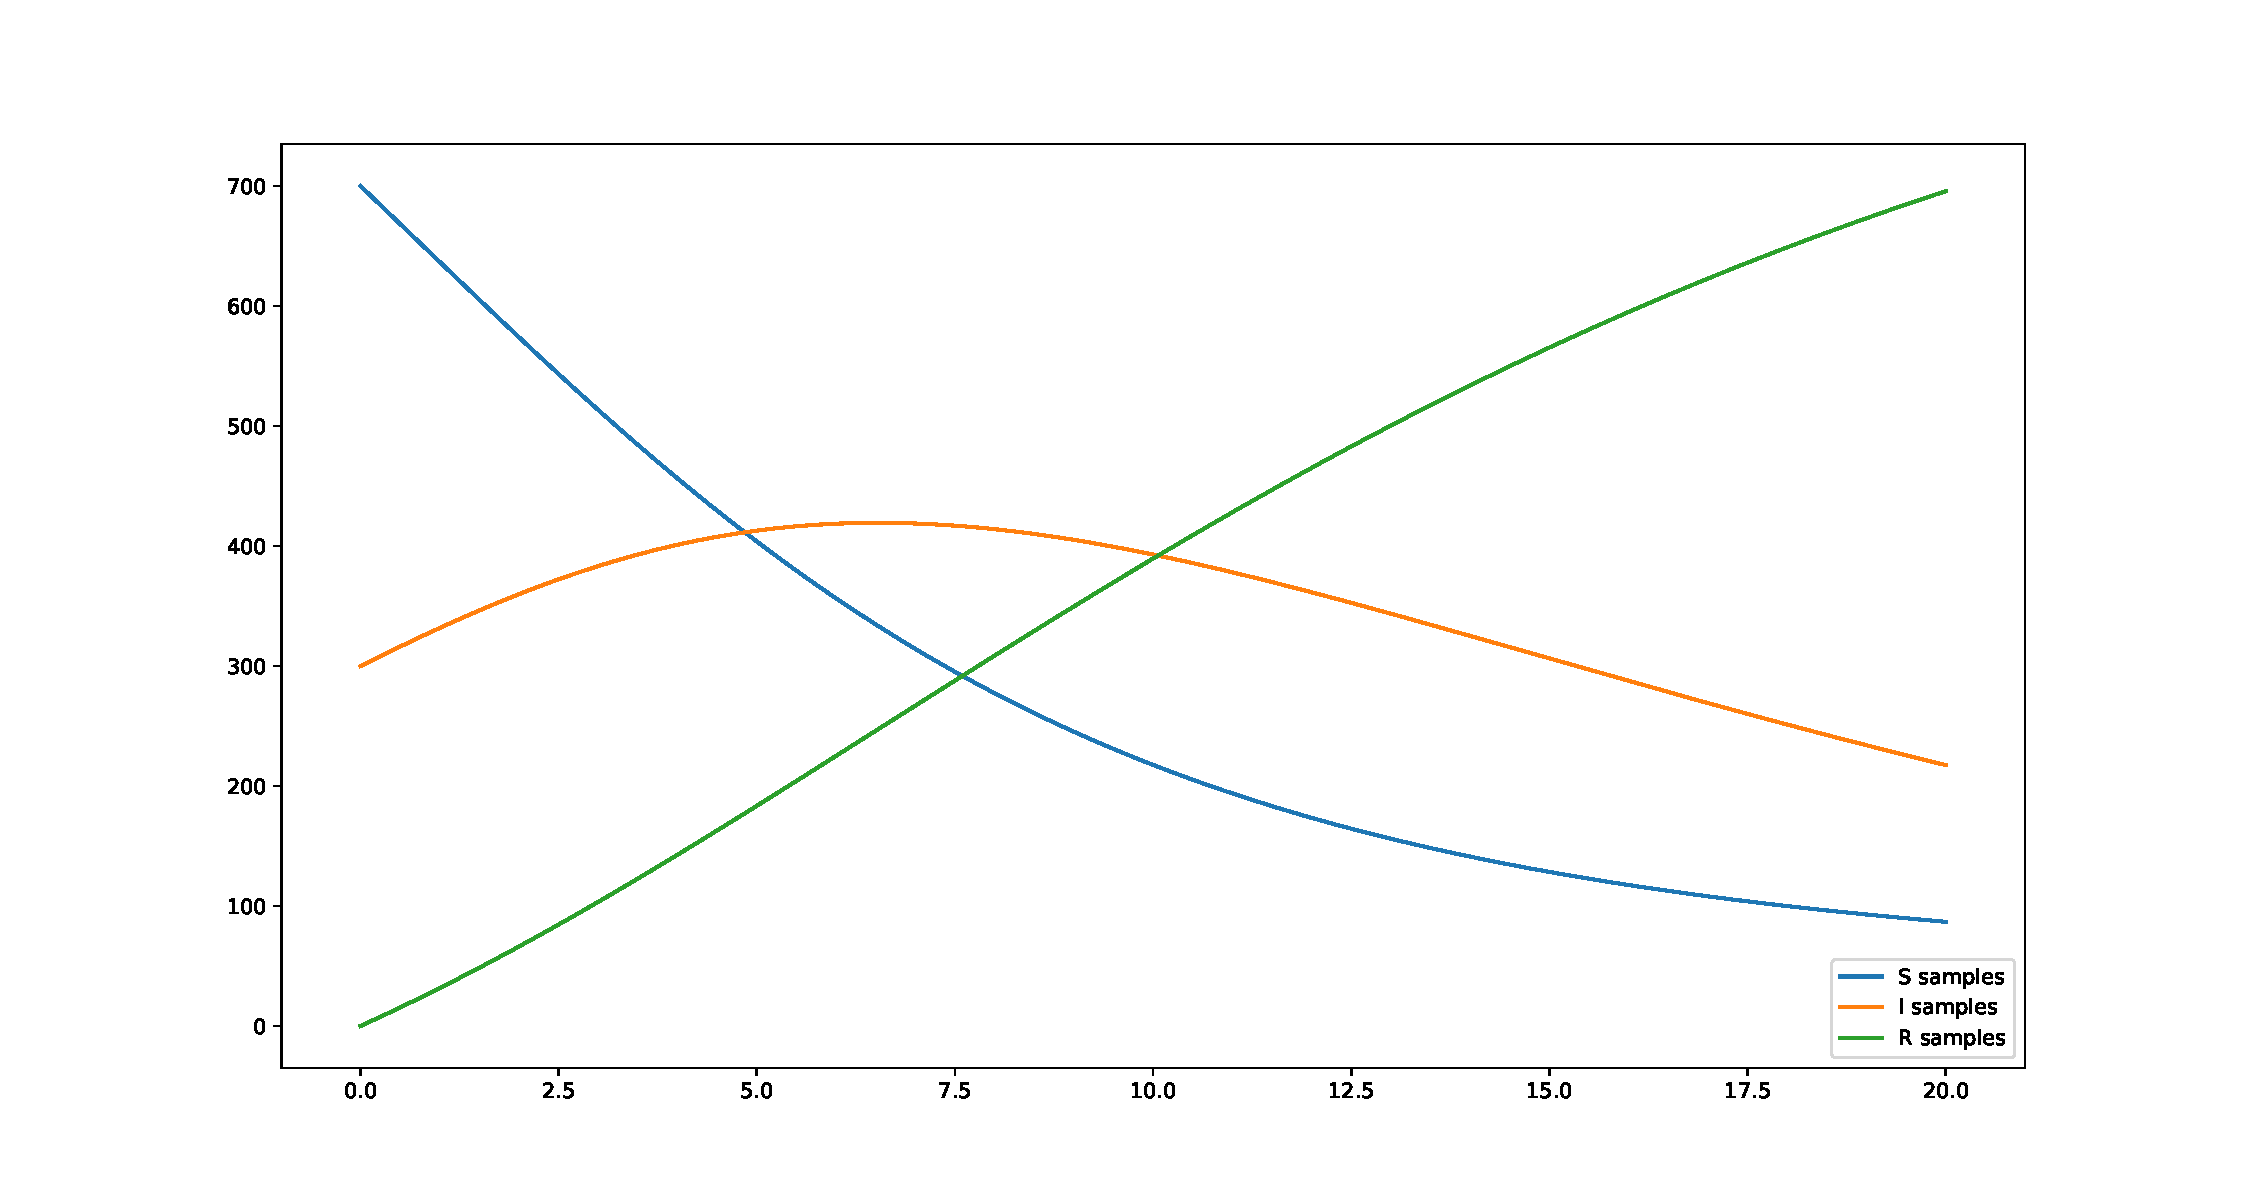
\includegraphics[width=\textwidth]{"figures/SIR.pdf"}
    \caption{modelo SIR con $a = 0.0003$, $b = 0.1$.}
    \label{fig:SIR}
\end{figure}

Cuando se tienen los datos de la forma $\{(t_i, y_i), i=1, \dots, n\}$ generados por la integración del modelo, se le agregan distintos valores de ruido a los puntos. A cada muestra $y_i$ se le agrega un valor de ruido utilizando la fórmula:

$$y_{i_{noise}} = y_i + y_i * max\_noise * random\_standard\_normal(),$$

donde $random\_standard\_normal()$ es una función que genera valores aleatorios normales, independientes, con media 0 y varianza 1. $Max\_noise$ es un parámetro con mínimo valor $0$ y máximo $1$ que define el ``ruido  máximo'' que se le agrega a cada muestra. Se puede ver el parámetro $max\_noise$ como el \% máximo del valor de cada muestra que se puede agregar como ruido. Durante los distintos experimentos se utilizaron como máximo ruido los valores de 0\%, 5\% o 10\% con respecto a cada muestra. Por ejemplo, si se agrega ruido a los datos obtenidos de la integración del sistema SIR utilizando el parámetro $max\_noise$ con valor $0.1$, se tendrían las curvas que aparecen en la imagen \ref{fig:SIR_with_noise} de la página \pageref{fig:SIR_with_noise}.

\begin{figure}[h]
    \centering
    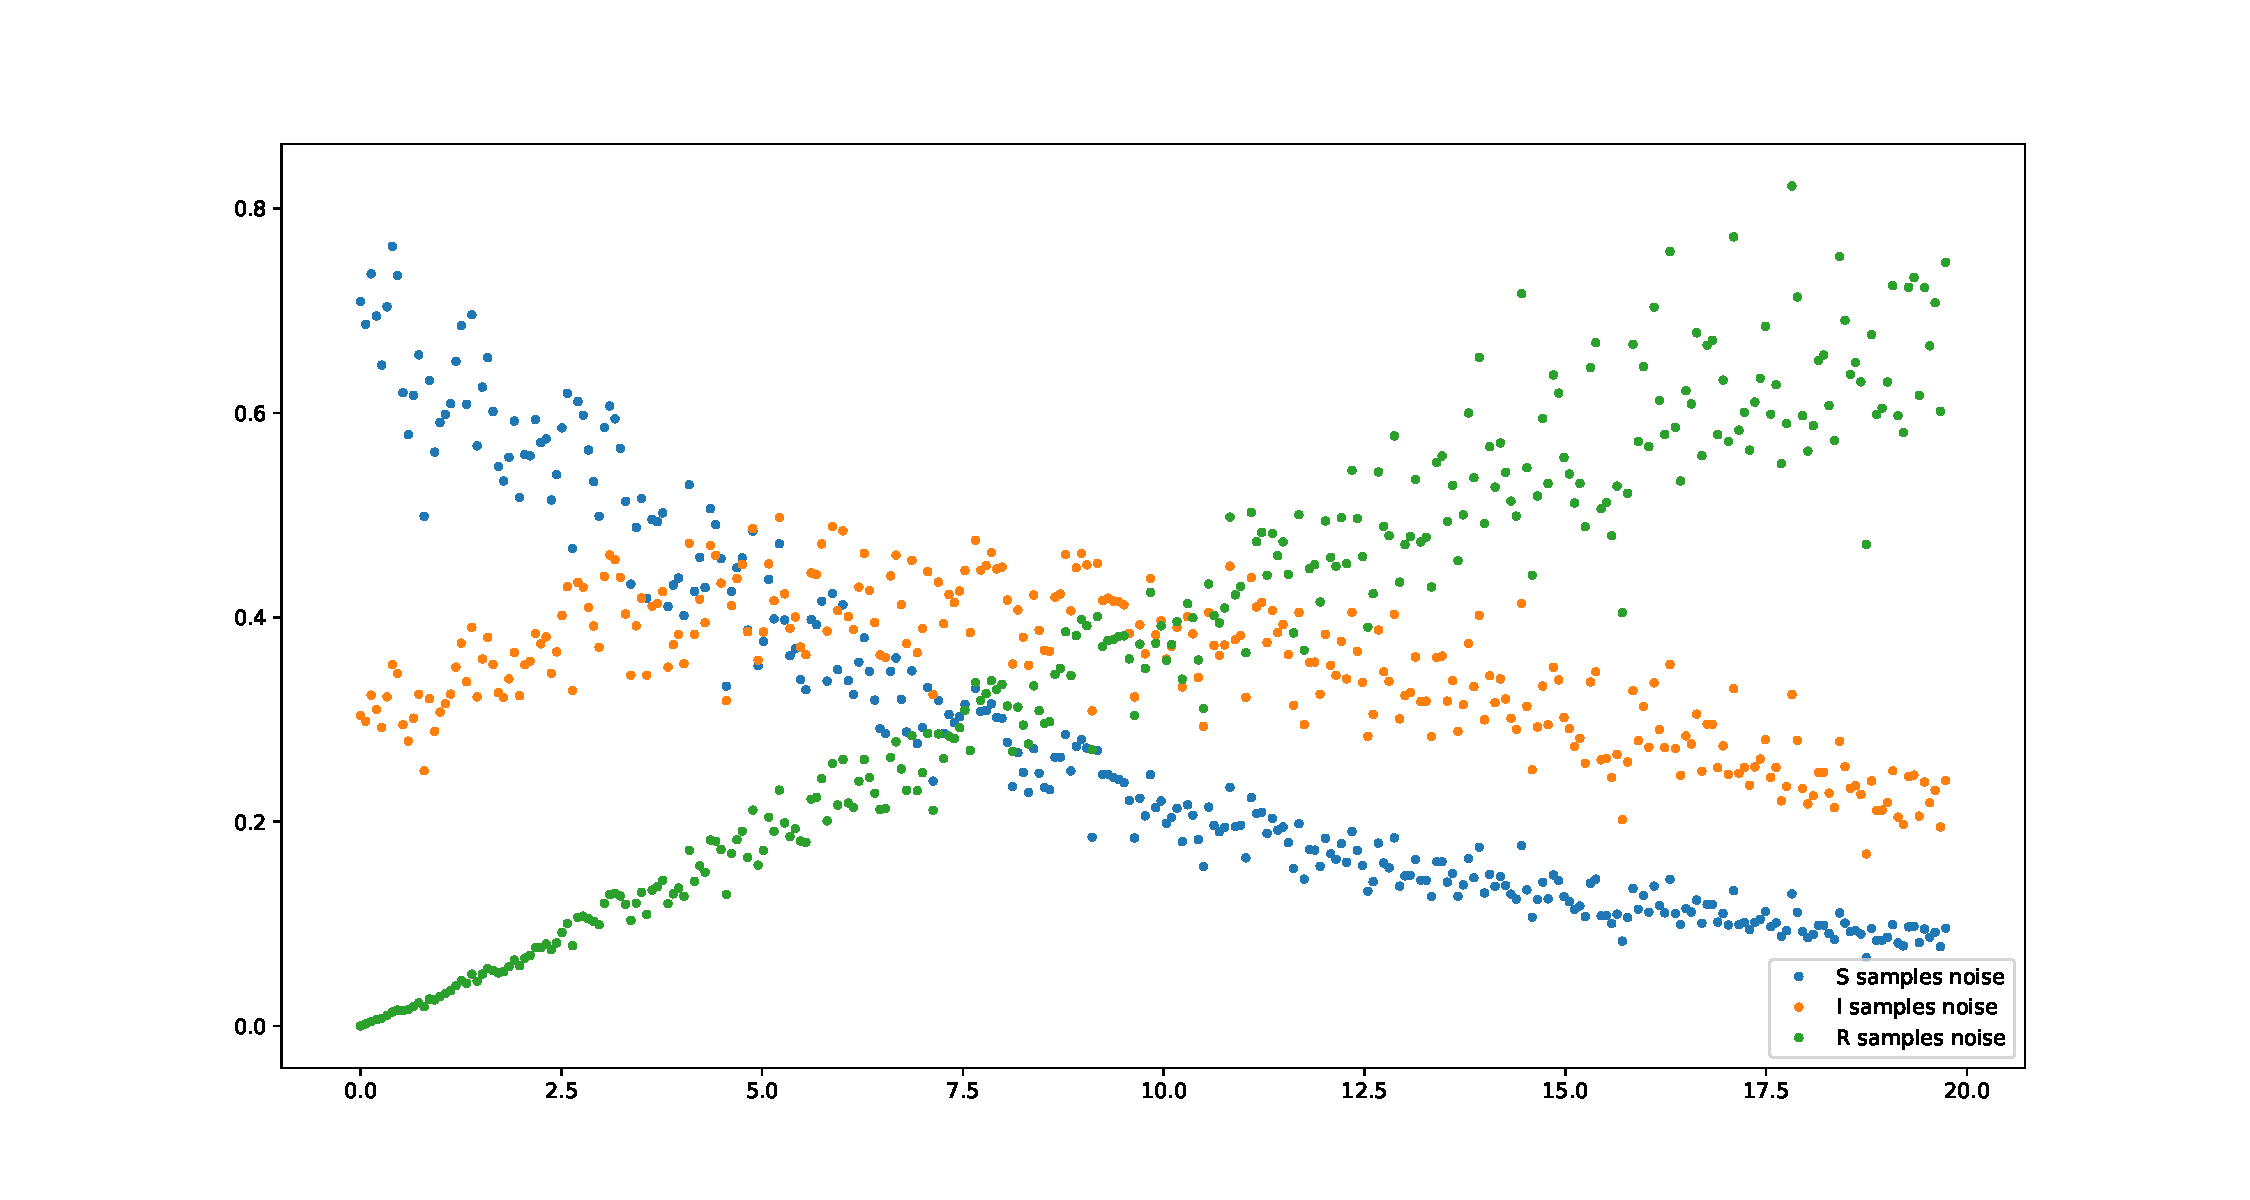
\includegraphics[width=\textwidth]{"figures/SIR_with_noise.pdf"}
    \caption{modelo SIR con $a = 0.0003$, $b = 0.1$ y $max\_noise = 0.1$.}
    \label{fig:SIR_with_noise}
\end{figure}

Cuando el valor de $max\_noise$ es mayor que 0, se usa un spline de suavizado para eliminar el ruido. El valor del parámetro de suavizado en el spline se varía para cada una de las variables. Por ejemplo, si se utiliza un spline de suavizado cúbico en los datos con ruido del sistema SIR se obtendrían las curvas que aparecen en la imagen \ref{fig:SIR_noise_with_spline} de la página \pageref{fig:SIR_noise_with_spline}.

\begin{figure}[h]
    \centering
    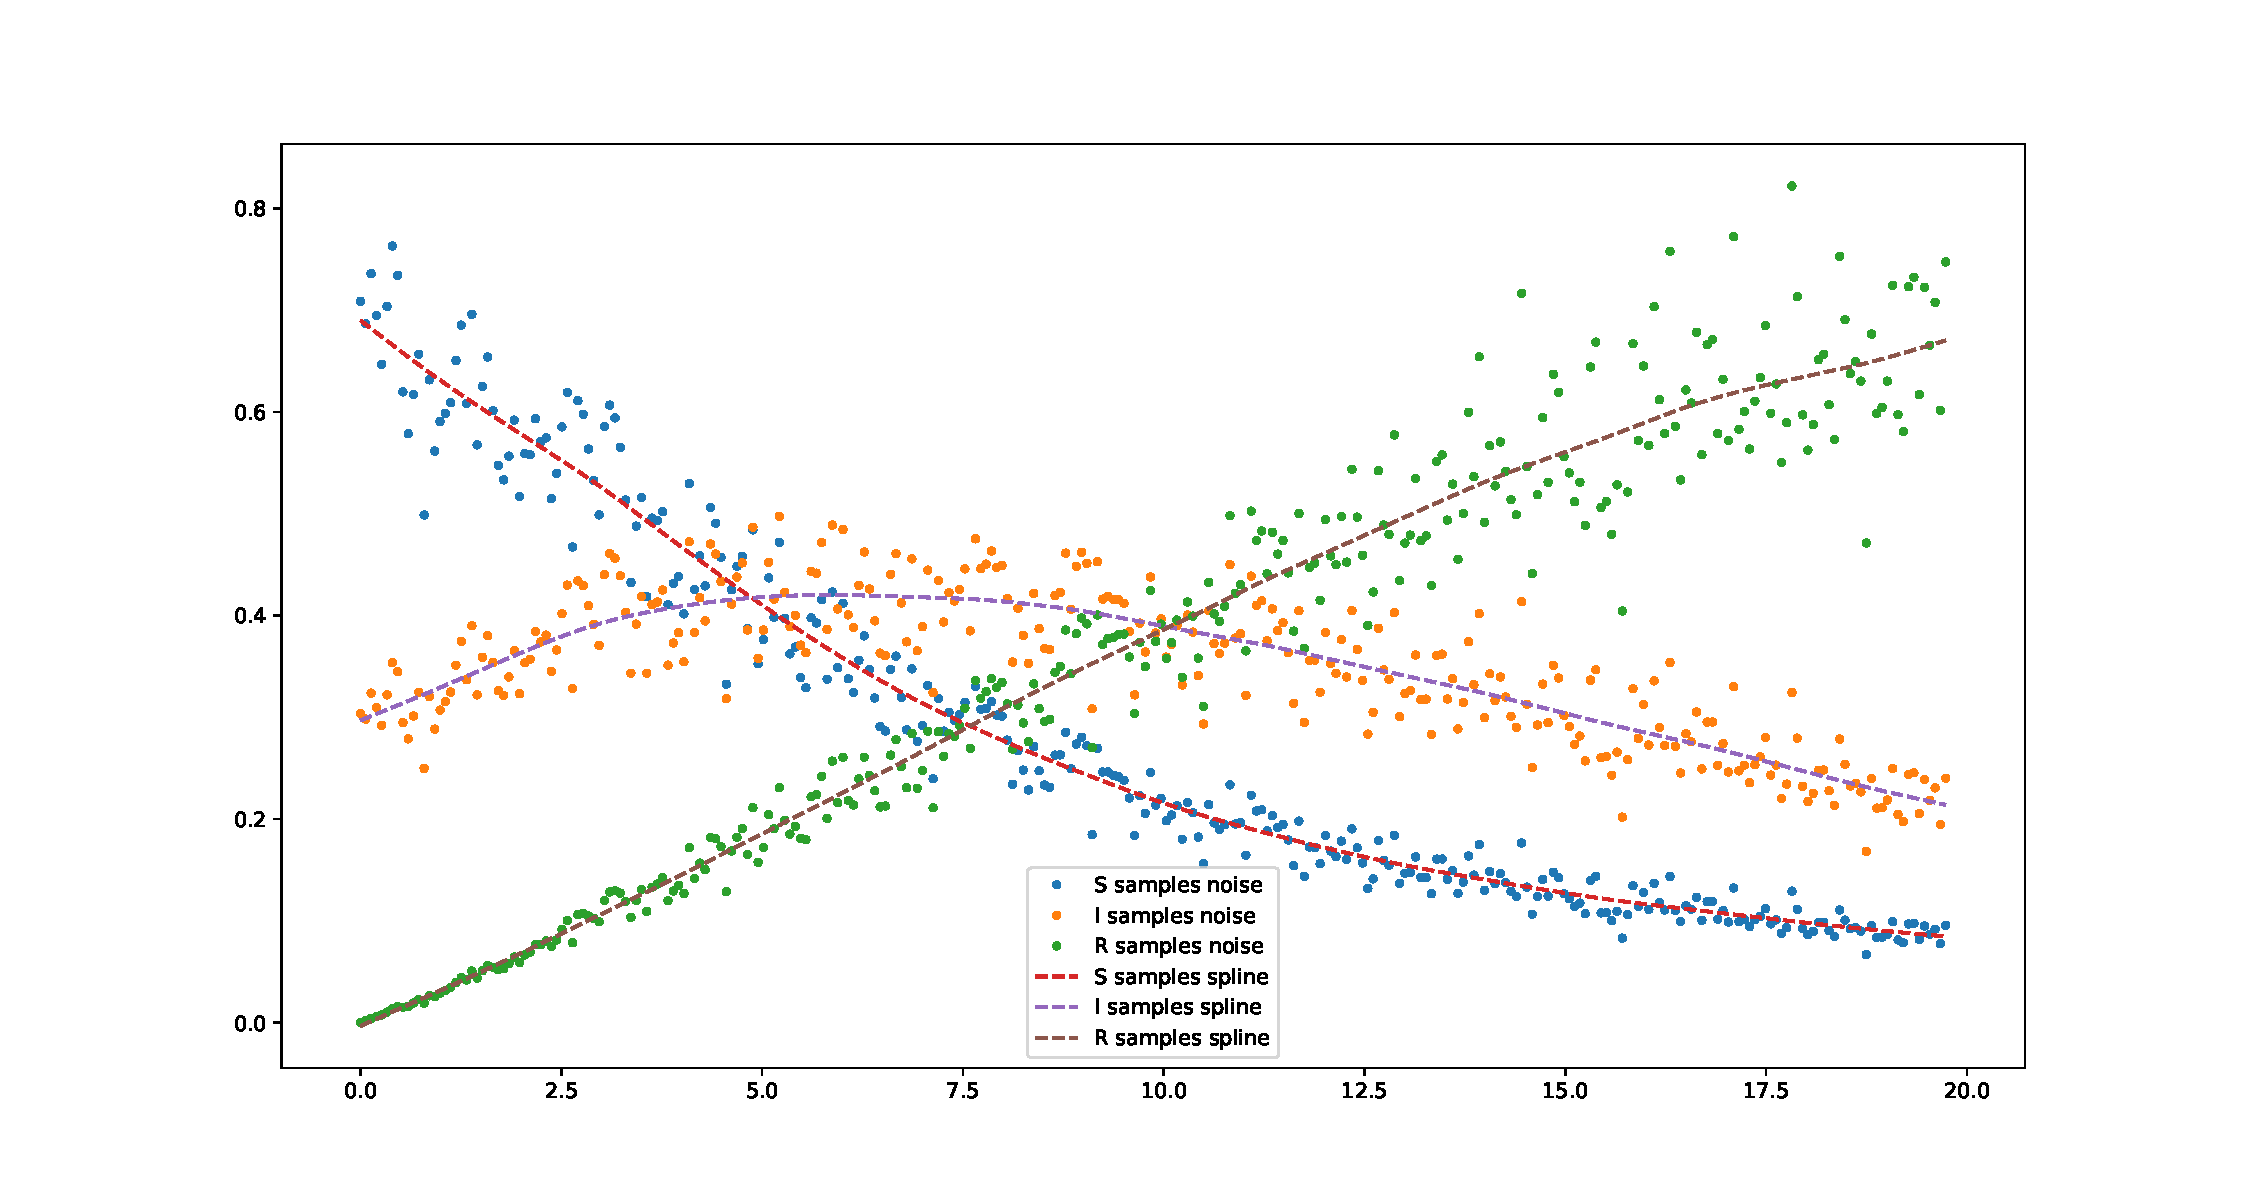
\includegraphics[width=\textwidth]{"figures/SIR_noise_with_spline.pdf"}
    \caption{modelo SIR con $a = 0.0003$, $b = 0.1$, $max\_noise = 0.1$ y smoothing-spline con valor de suavizado de $0.1$.}
    \label{fig:SIR_noise_with_spline}
\end{figure}

Una vez que se tiene el spline de suavizado, se puede aproximar el valor de la función $y_i$. Como lo que se busca es generar un conjunto de datos de la forma:

$$\{(t_i, y_i, y'_i), i=1, \dots, n\},$$

para obtener $f(t_i, y_i)$ mediante el uso de la regresión simbólica, se puede generar una aproximación del valor de $y'_i$ utilizando la primera derivada del spline.

En las siguientes secciones se presentan los experimento en los que se utiliza la regresión simbólica para encontrar el sistema de ecuaciones diferenciales lineales con respecto a los parámetros a partir de un conjunto de datos generado. Se utilizaron en total 5 modelos para la generación de los disintos conjuntos de datos que fueron el sistema de lotka volterra \cite{Hoppensteadt:2006}, SIR \cite{weiss2013sir}, SIRD \cite{bailey1975mathematical}, SIQRD \cite{molter2021mathematical} y SVVEIR \cite{kuddus2021mathematical}.

\section{Experimentos realizados}\label{section:experiments}

Todos los sistemas de ecuaciones diferenciales seleccionados para los experimentos son sistemas lineales con respecto a los parámetros. La cantidad de ecuaciones en cada uno de los modelos es distinta. De cada modelo se muestra una tabla que contiene la media del valor de la función de ajuste a lo largo de las 30 ejecuciones del experimento así como el mínimo y máximo valor que alcanzó el error cuadrático medio.

Por cada experimento en el que se utiliza el modelo $f$, se genera un conjunto de datos $S$ de la forma $\{(t_i, y_i), i=1, \dots, n\}$ mediante la integración del modelo. Luego se crea el conjunto de datos $y_{noise_{x\%}}$ resultantes de agregarle ruido al conjunto $S$ con $max\_noise=x$ y se define $y_{spline_{x\%}}$ como los datos resultantes de la aproximación de la función $y$ a partir de los datos $y_{noise_{x\%}}$. Con todos estos datos se genera el sistema $\hat{f}$ utilizando la regresión simbólica. Se define el conjunto de datos $y_{sr_{x\%}}$ como los datos generados por la integración del sistema encontrado en la regresión simbólica. Además se tiene el sistema $f_{pso}$ como el resultado de aplicar el método $PSO$ \cite{p-pso-6} utilizando el conjunto $S$.

De todos los experimentos en los que se utiliza el modelo $f$ solo se tuvieron en cuenta en los resultados un conjunto de los 30 experimentos realizado. Esta cantidad que se tiene en cuenta se define en la fila ``cantidad de sistemas'' de la tabla de resultados con la forma \ref{table:experiment_form} que aparece en la página \pageref{table:experiment_form}.

\begin{table}
    \centering
    \caption{Estructura de tabla de resultados.}
    \begin{tabular}{|c|c|}
        \hline
                             & \textbf{ruido de x\%}                                                      \\
        \hline
        cantidad de sistemas & $m$                                                                        \\
        \hline
        original             & $\frac{\frac{\sum_{i=1}^n (y_i-y_{sr_{x\%}})^2}{n}}{m}$                    \\
        \hline
        original con ruido   & $\frac{\frac{\sum_{i=1}^n (y_{noise_{x\%}}-y_{sr_{x\%}})^2}{n}}{m}$        \\
        \hline
        spline               & $\frac{\frac{\sum_{i=1}^n (y_{spline_{x\%}}-y_{sr_{x\%}})^2}{n}}{m}$       \\
        \hline
        otro método          & $\frac{\frac{\sum_{i=1}^n (f_{PSO}(t_i, y_i)-\hat{f}(t_i, y_i))^2}{n}}{m}$ \\
        \hline
    \end{tabular}
    \label{table:experiment_form}
\end{table}

A continuación se muestra el experimento realizado a partir de la generación de los datos utlizando el sistema Lotka-Volterra.

\subsection{Lotka-Volterra}

El modelo de Lotka-Volterra es un sistema utilizado para describir las interacciones entre dos especies, una como depredador y otra como presa \cite{Hoppensteadt:2006}. La población de cada especie cambia a través del tiempo de acuerdo al sistema de ecuaciones diferenciales:

\begin{align*}
    X' & = X (a - b Y)   \\
    Y' & = -Y (c - d X).
\end{align*}

Se utilizaron como valores de los parámetros $a = 0.04$, $b = 0.0005$, $c = 0.2$ y $d = 0.004$ con punto inicial $(20, 20)$ y se integró en el intervalo $0 \leq t \leq 300$ para obtener los datos que aparecen en la figura \ref{fig:lotka_volterra} de la página \pageref{fig:lotka_volterra}. Del conjunto de puntos se seleccionaron 300 muestras como datos para el método de regresión simbólica.

\begin{figure}[h]
    \centering
    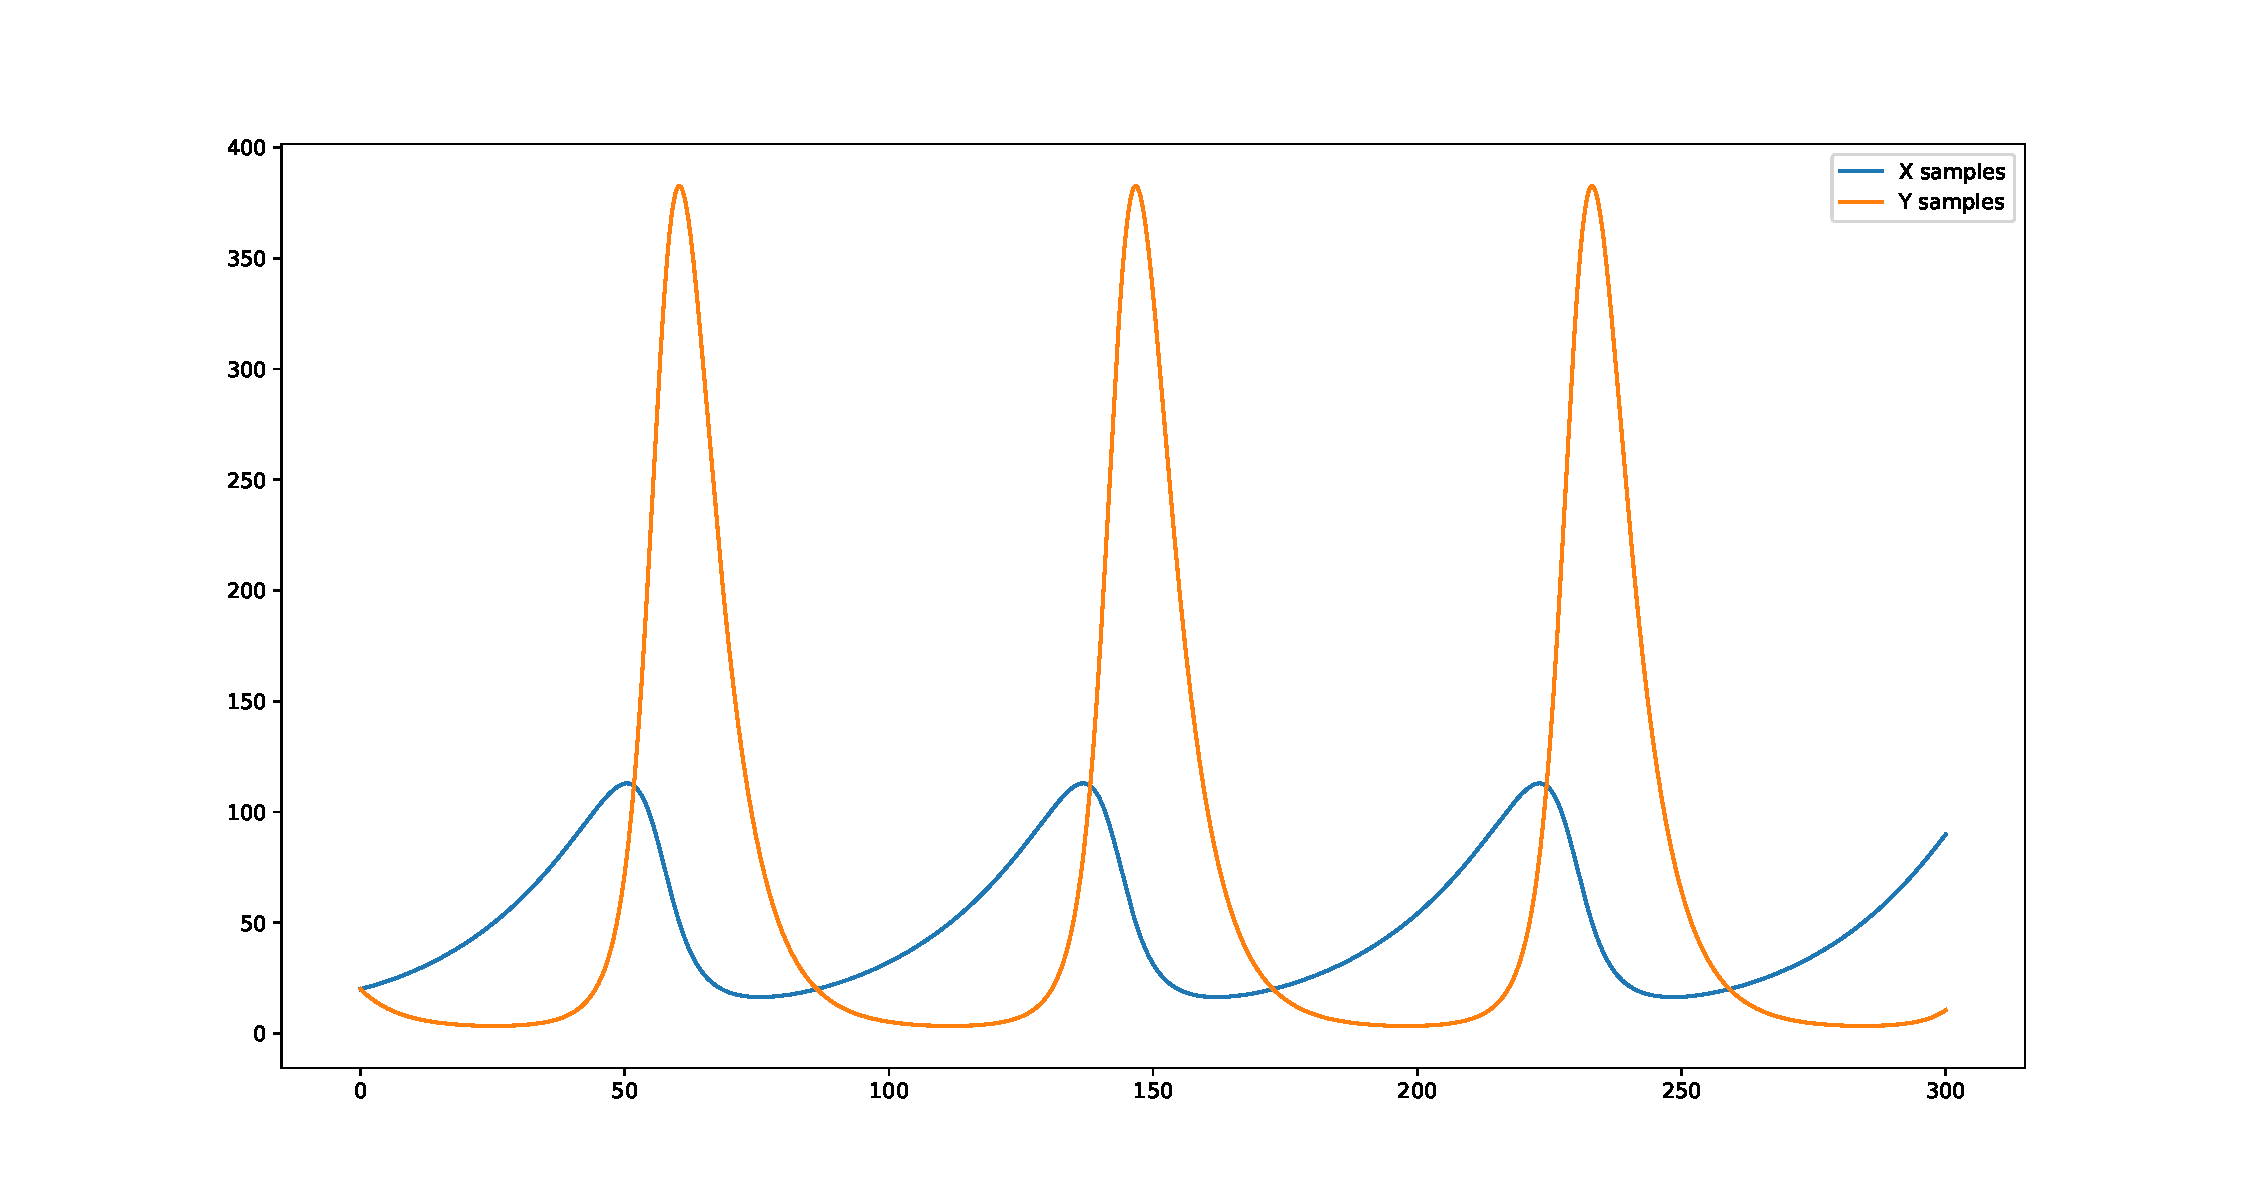
\includegraphics[width=\textwidth]{"figures/lotka_volterra.pdf"}
    \caption{modelo Lotka Volterra con $a = 0.04$, $b = 0.0005$, $c = 0.2$ y $d = 0.004$.}
    \label{fig:lotka_volterra}
\end{figure}

Los resultados que se obtienen durante las 30 ejecuciones del experimento aparecen en la tablas \ref{table:experiment_lotka_volterra}.

\begin{table}[!h]
    \centering
    \caption{Resultados que se obtienen en el modelo Lotka-Volterra.}

    \begin{tabular}{|c|c|c|c|}
        \hline
               & \textbf{ruido de 0\%} & \textbf{ruido de 5\%} & \textbf{ruido de 10\%} \\
        \hline
        media  & 0.74514               & 0.69138               & 0.84485                \\
        \hline
        mínimo & 0.28343               & 0.42189               & 0.54373                \\
        \hline
        máximo & 0.97944               & 1.11027               & 1.68603                \\
        \hline
    \end{tabular}

    \begin{tabular}{|c|c|c|c|c|c|}
        \hline
                             & \textbf{ruido de 0\%} & \textbf{ruido de 5\%} & \textbf{ruido de 10\%} \\
        \hline
        cantidad de sistemas & 30                    & 28                    & 25                     \\
        \hline
        original             & 17.01575              & 52.17101              & 50.30572               \\
        \hline
        original con ruido   & 17.01575              & 52.21558              & 50.56727               \\
        \hline
        spline               & 17.01575              & 51.85661              & 49.99422               \\
        \hline
        otro método          & 1394.26981            & 1111.95166            & 1519.66141             \\
        \hline
    \end{tabular}

    \label{table:experiment_lotka_volterra}
\end{table}

Durante la realización de los experimentos el modelo de lotka-volterra, la regresión simbólica encontró el sistema que generó los datos pero con otros parámetros en 21 ocasiones cuando no se utilizaba ruido en los datos, 13 veces cuando se utilizó un ruido máximo de 5\% y 6 veces cuando se utilizó un ruido máximo de 10\%. En las figuras \ref{fig:final_plot_LV_0.0} de la página \pageref{fig:final_plot_LV_0.0}, \ref{fig:final_plot_LV_0.05} de la página \pageref{fig:final_plot_LV_0.05} y \ref{fig:final_plot_LV_0.1} de la página \pageref{fig:final_plot_LV_0.1} se pueden ver los datos originales comparados con los datos obtenidos del mejor resultado generado por la regresión simbólica.

\begin{figure}[h]
    \centering
    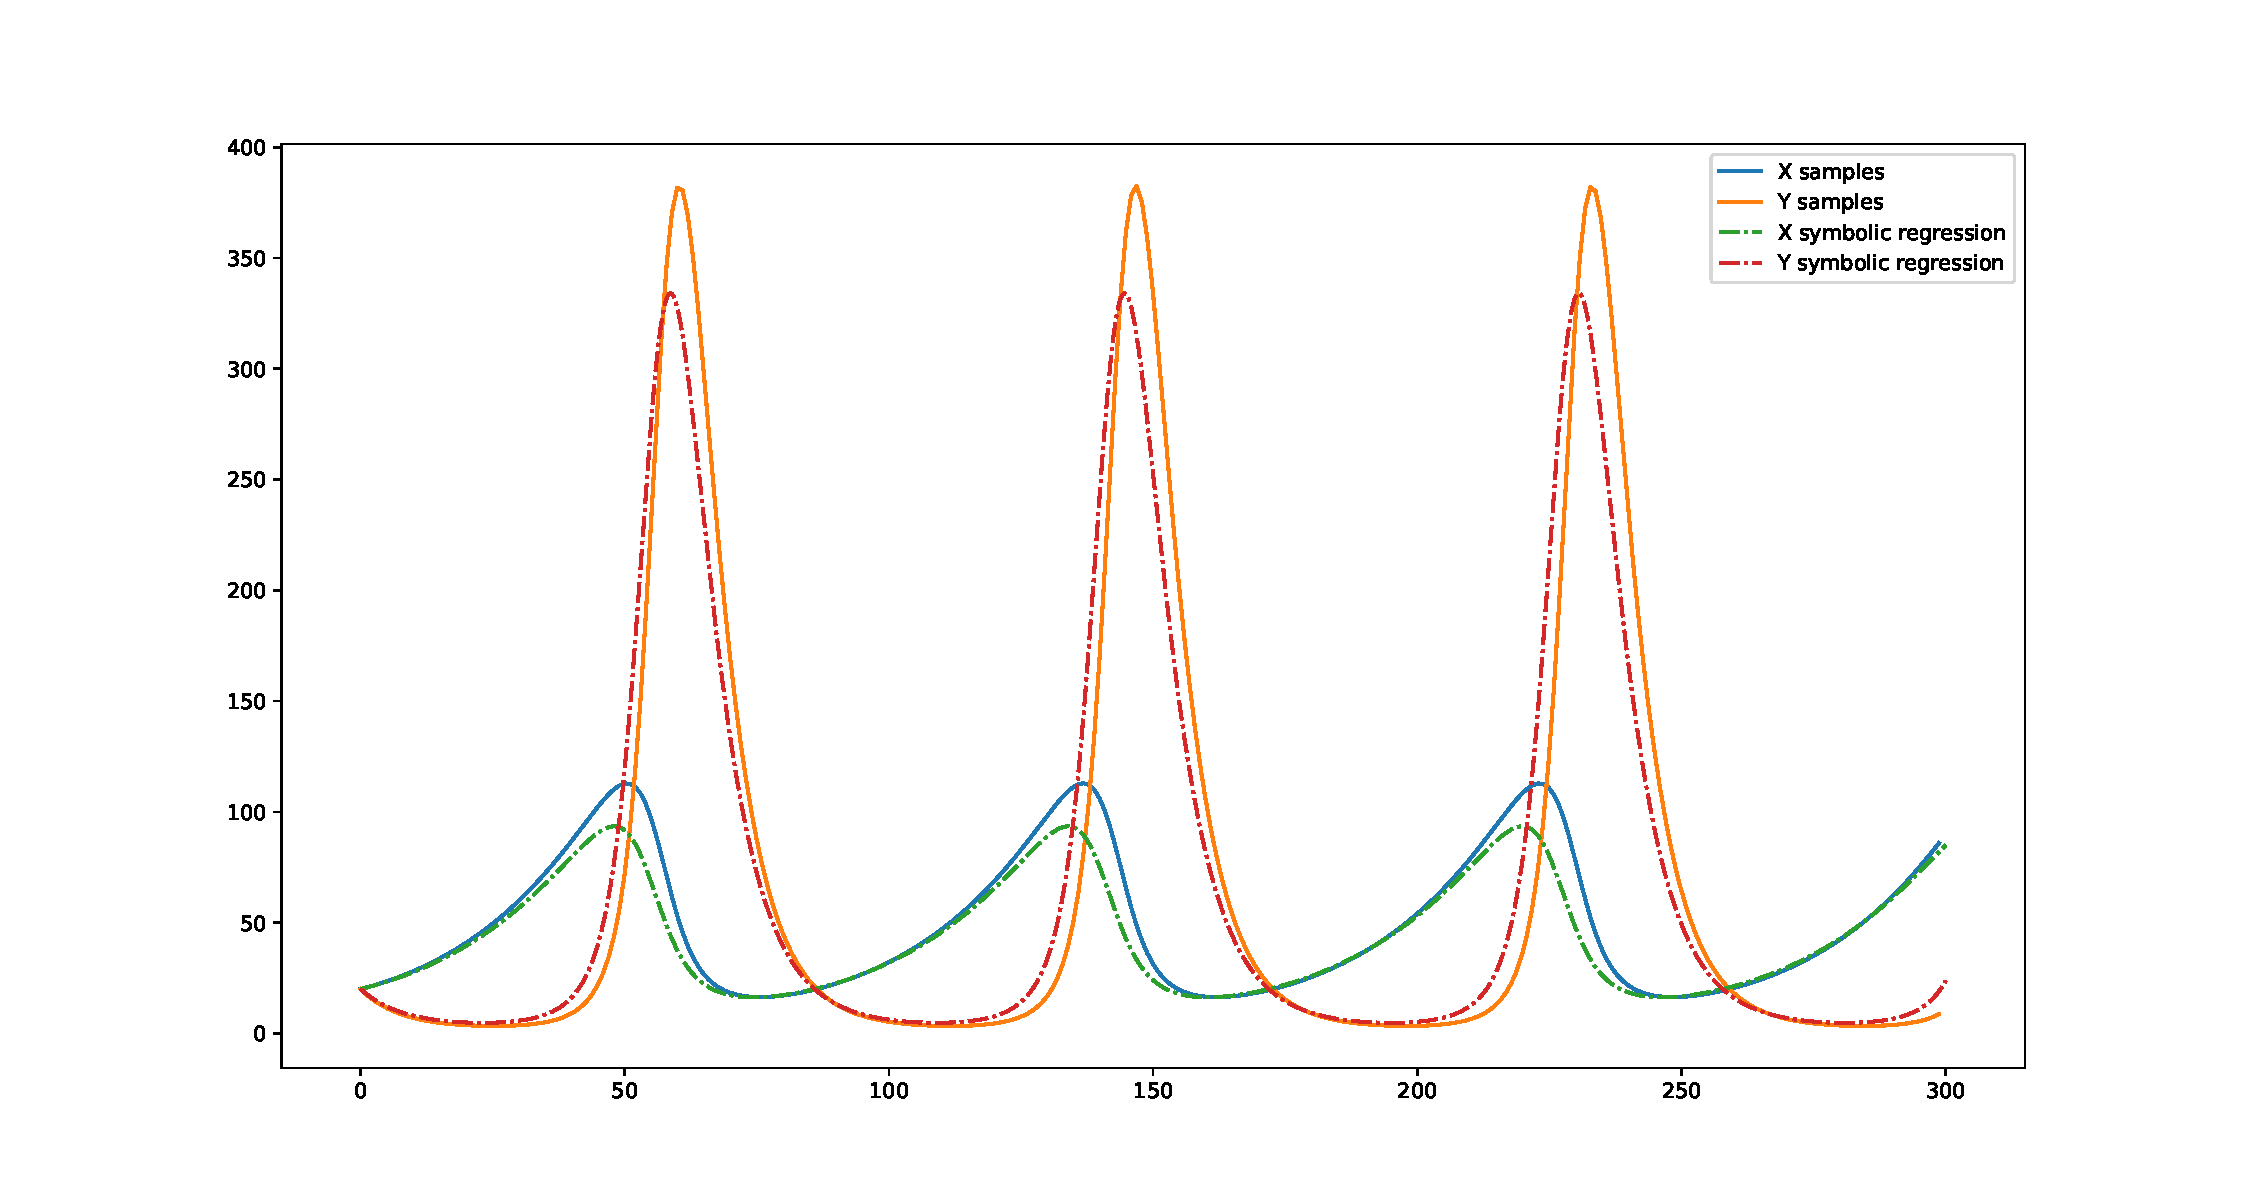
\includegraphics[width=\textwidth]{"figures/final_plot_LV_0.0.pdf"}
    \caption{Modelo resultante utilizando datos generados a partir del modelo lotka-volterra con ruido máximo de 0\%.}
    \label{fig:final_plot_LV_0.0}
\end{figure}

\begin{figure}[h]
    \centering
    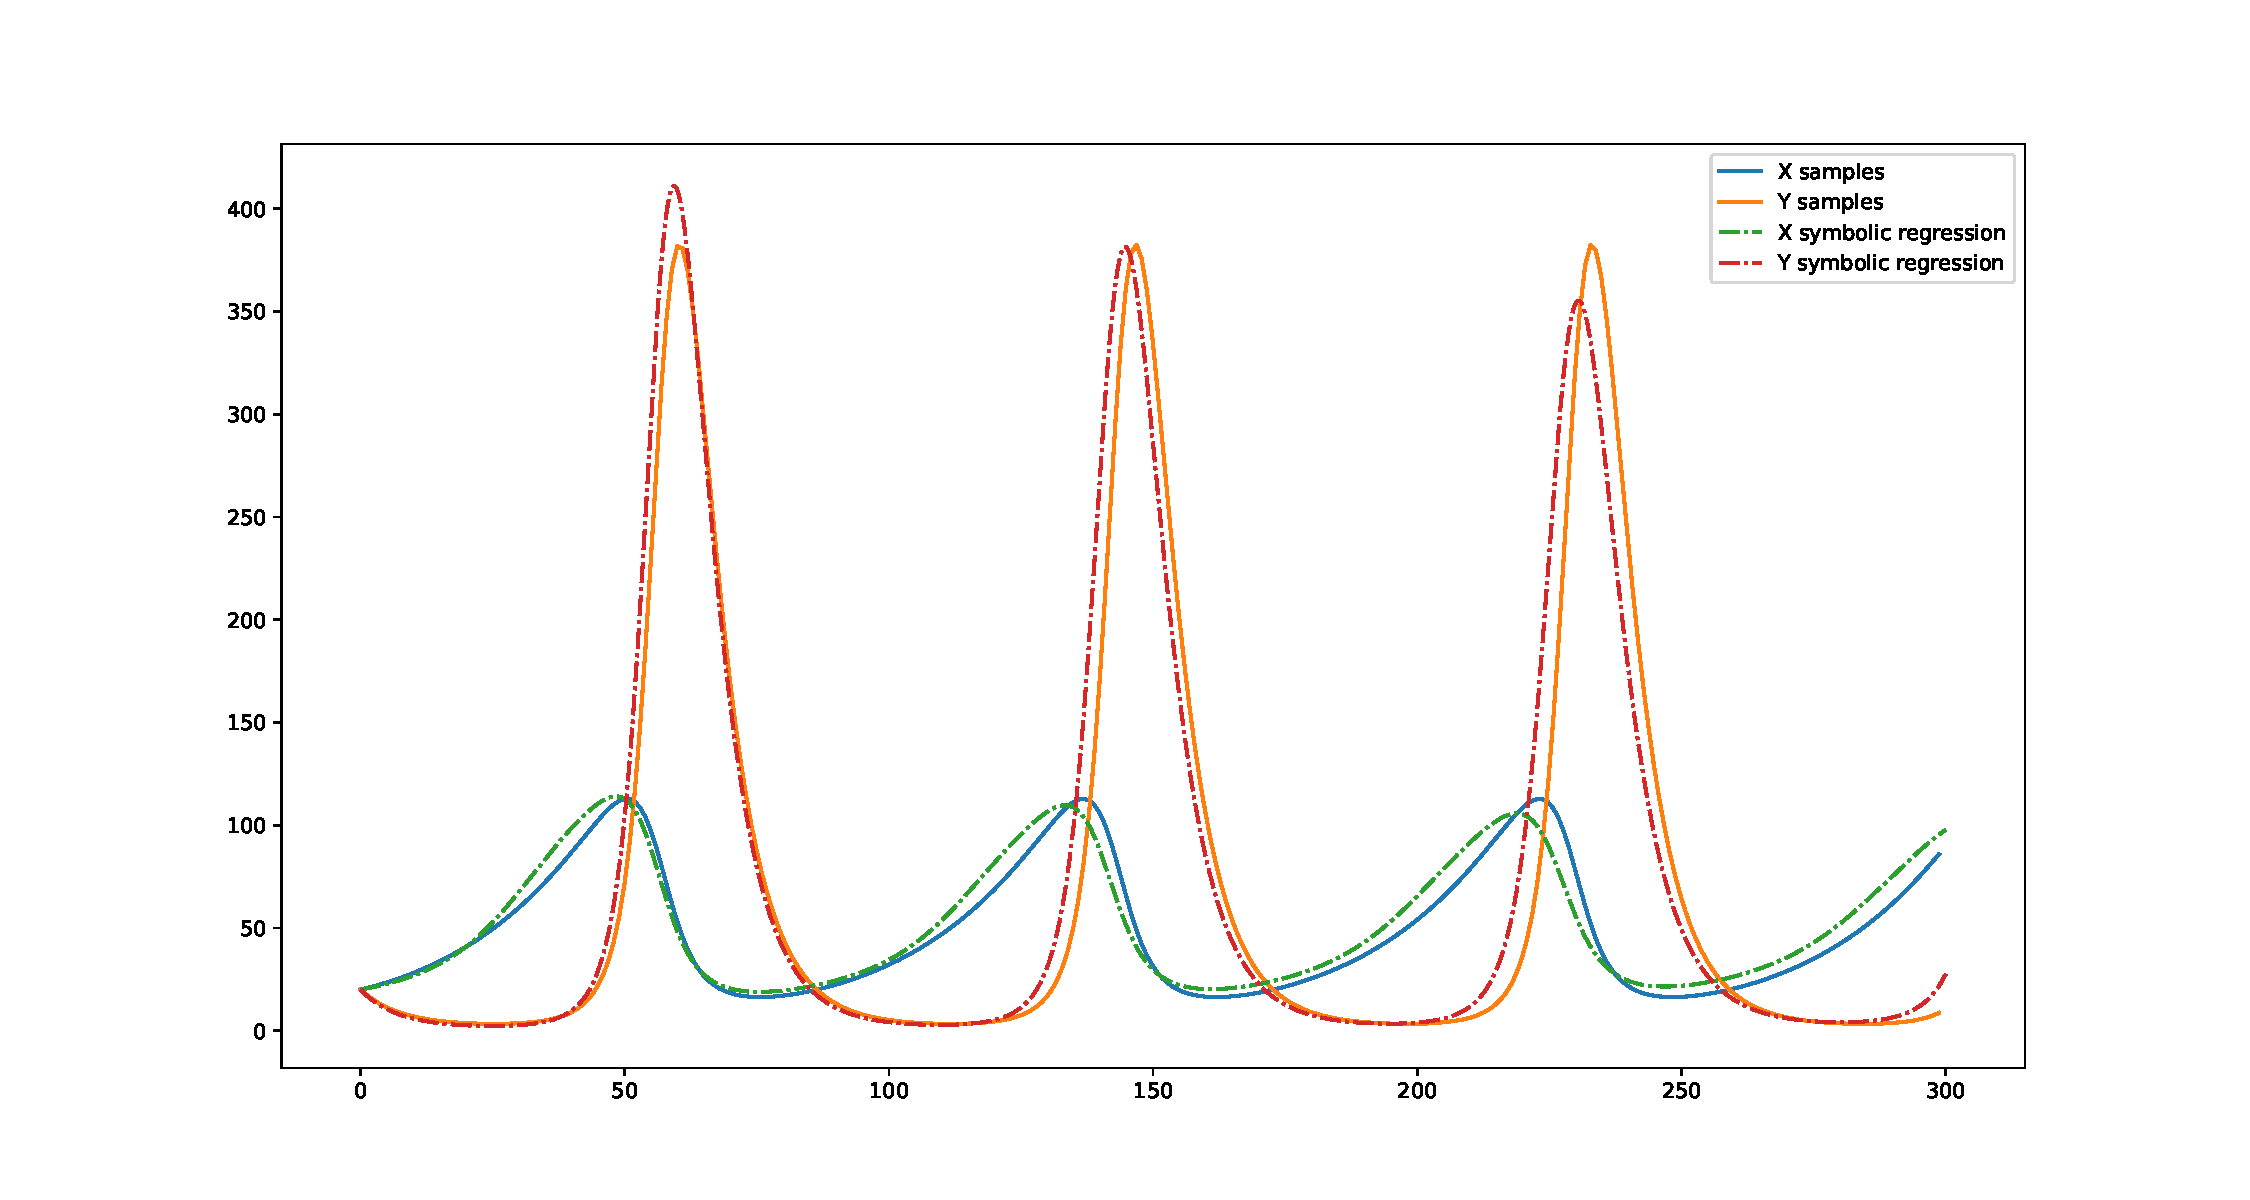
\includegraphics[width=\textwidth]{"figures/final_plot_LV_0.05.pdf"}
    \caption{Modelo resultante utilizando datos generados a partir del modelo lotka-volterra con ruido máximo de 5\%.}
    \label{fig:final_plot_LV_0.05}
\end{figure}

\begin{figure}[h]
    \centering
    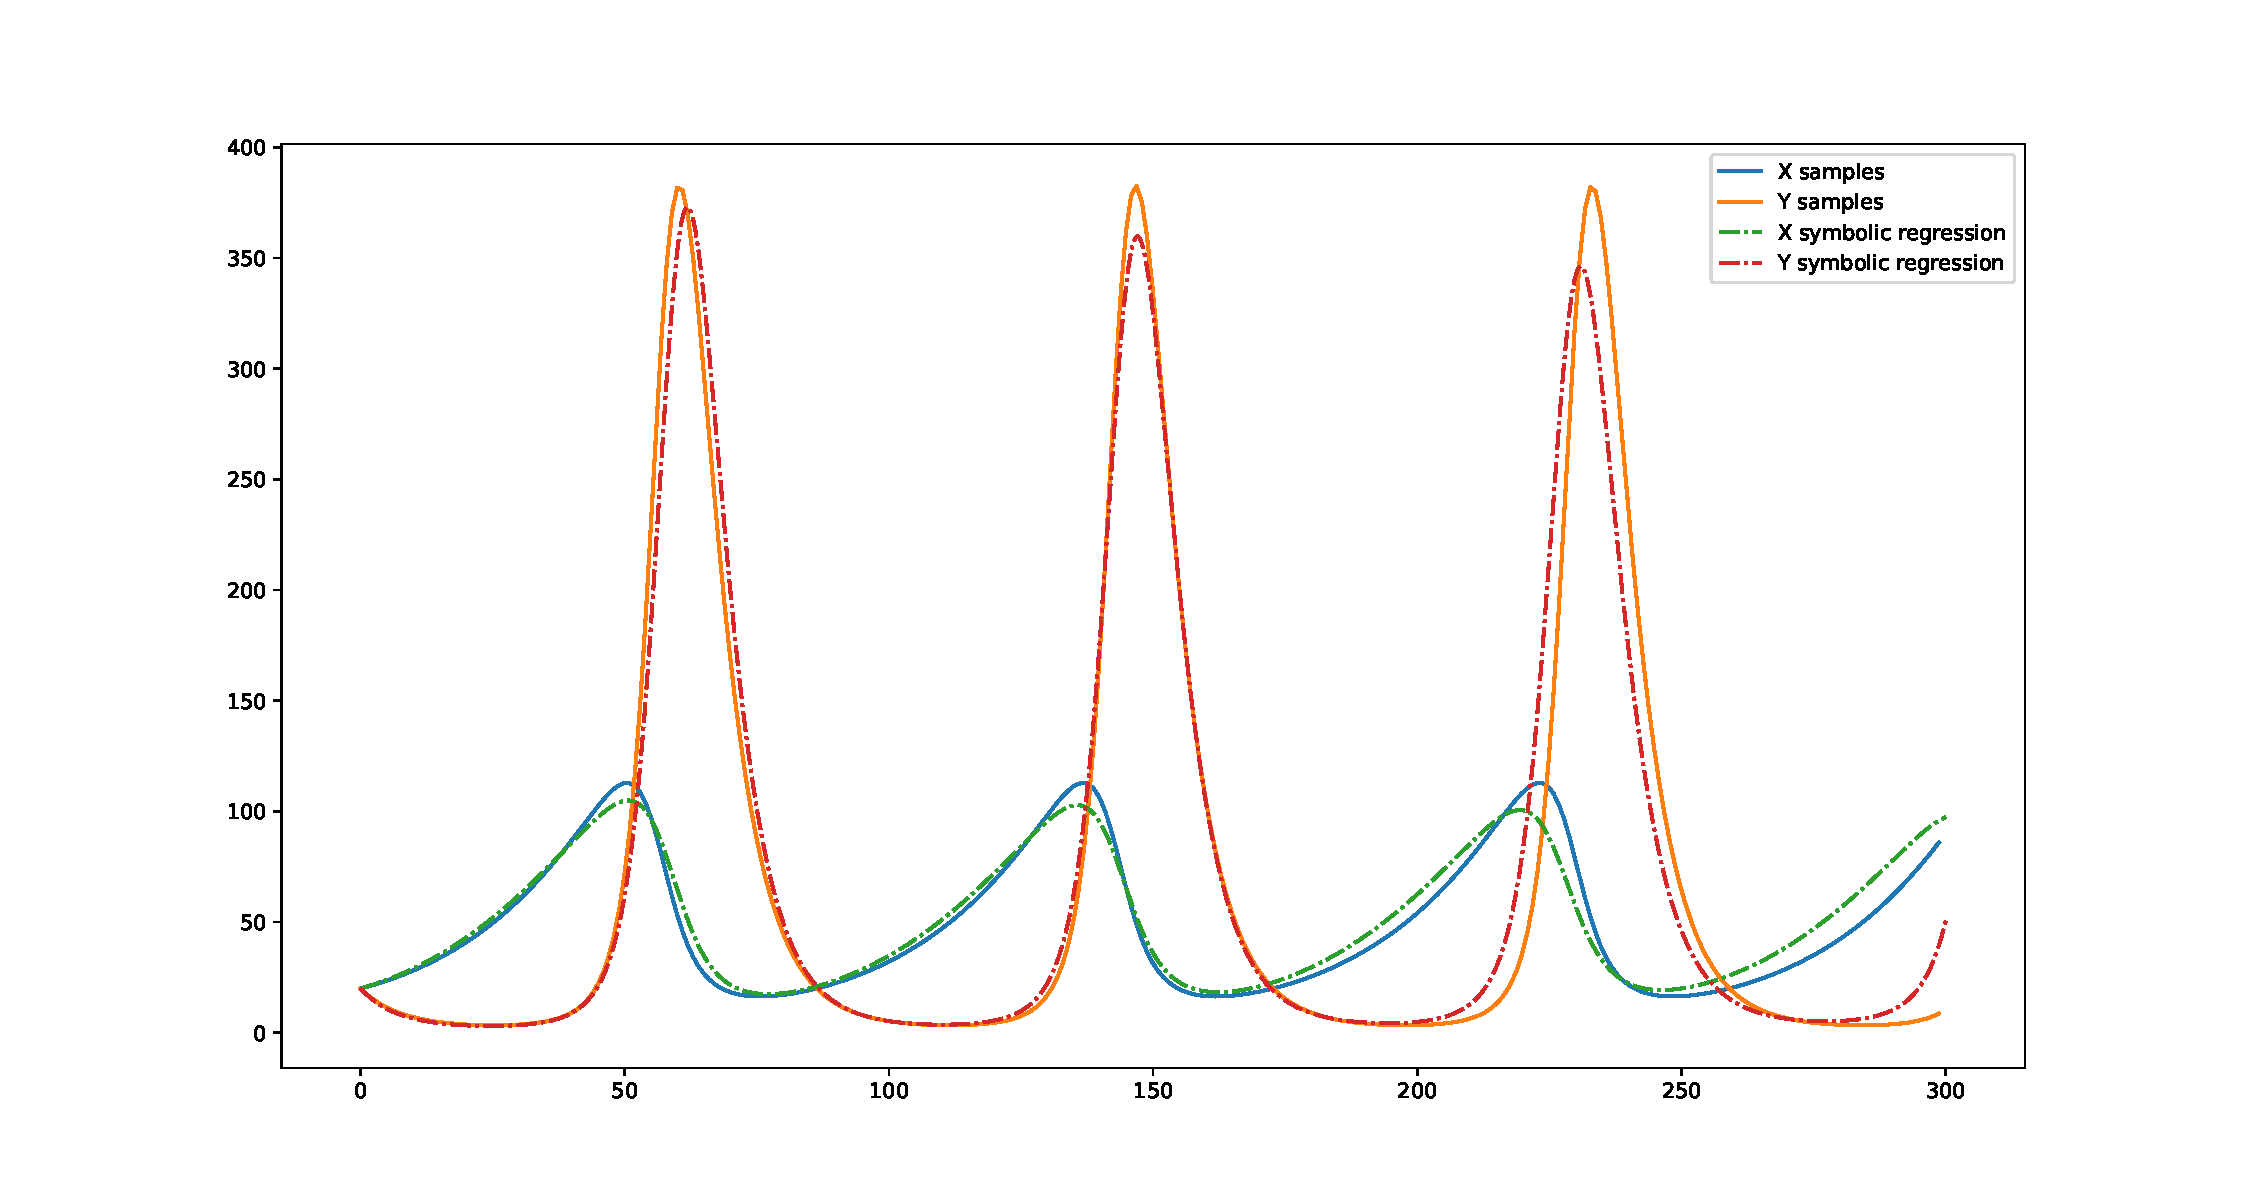
\includegraphics[width=\textwidth]{"figures/final_plot_LV_0.1.pdf"}
    \caption{Modelo resultante utilizando datos generados a partir del modelo lotka-volterra con ruido máximo de 10\%.}
    \label{fig:final_plot_LV_0.1}
\end{figure}


En el resto de experimentos realizados utilizando otros modelos, nunca se obtuvo como resultado de la regresión simbólica el modelo original que generó los datos.

Si en lugar de utilizar como aproximación el método de diferencias finitas cuando los datos no poseen ruido, se utiliza el sistema original de Lotka-Volterra, se obtiene que la media del valor de la función de ajuste a lo largo de las 30 ejecuciones del experimento es $0.00721$. El valor máximo de la función de ajuste alcanzado fue de $0.21654$ y el mínimo de $6.35015e-16$, en este último la regresión simbólica obtuvo exactamente el sistema utilizado para generar los datos.


A continuación se muestra el experimento realizado a partir de la generación de los datos utilizando el sistema SIR.

\subsection{SIR}

El modelo SIR es un sistema que se utiliza para describir la transmición de una enfermedad infecciosa causada por una bacteria, virus u hongos. \cite{weiss2013sir}. El sistema se define como:

\begin{align*}
    S' & = - aIS    \\
    I' & = aIS - bI \\
    R' & = bI,
\end{align*}

donde $S$ indica la cantidad de personas susceptibles, $I$ la cantidad de personas infectadas y $R$ la cantidad de personas recuperadas. Se utiliza el parámetro $a$ para indicar el índice de transmición y $b$ el índice de recuperación de la enfermedad.

Se utilizaron como valores de los parámetros $a = 0.0003$ y $b = 0.1$ con punto inicial $(700, 300, 0)$ y se integró en el intervalo $0 \leq t \leq 20$ para obtener los datos que aparecen en la imagen \ref{fig:SIR} de la página \pageref{fig:SIR}. Del conjunto de puntos se seleccionaron 300 muestras como datos para el método de regresión simbólica.

Los resultados que se obtienen durante las 30 ejecuciones del experimento, utilizando solamente en cada ecuación las variables permitidas según el modelo, aparecen en la tabla \ref{table:experiment_SIR} de la página \pageref{table:experiment_SIR}. Si se permite cualquier variable del modelo en cualquier ecuación del sistema se obtienen los datos que aparecen en la tabla \ref{table:experiment_SIR_all} de la página \pageref{table:experiment_SIR_all}.

\begin{table}[!h]
    \centering
    \caption{Resultados que se obtienen en el modelo SIR restringiendo las variables que aparecen en cada ecuación.}
    \begin{tabular}{|c|c|c|c|}
        \hline
               & \textbf{ruido de 0\%} & \textbf{ruido de 5\%} & \textbf{ruido de 10\%} \\
        \hline
        media  & 0.25506               & 4.78621               & 6.9987                 \\
        \hline
        mínimo & 0.2187                & 0.79521               & 1.48455                \\
        \hline
        máximo & 0.30485               & 31.77664              & 51.66934               \\
        \hline
    \end{tabular}

    \begin{tabular}{|c|c|c|c|c|c|}
        \hline
                             & \textbf{ruido de 0\%} & \textbf{ruido de 5\%} & \textbf{ruido de 10\%} \\
        \hline
        cantidad de sistemas & 30                    & 28                    & 28                     \\
        \hline
        original             & 2.02689               & 60.79755              & 117.71809              \\
        \hline
        original con ruido   & 2.02689               & 66.59004              & 130.68564              \\
        \hline
        spline               & 2.02689               & 61.046                & 117.83595              \\
        \hline
        otro método          & 31160.12619           & 27363.87727           & 35775.36901            \\
        \hline
    \end{tabular}
    \label{table:experiment_SIR}
\end{table}

\begin{table}[!h]
    \centering
    \caption{Resultados que se obtienen en el modelo SIR sin restringir las variables que aparecen en cada ecuación.}
    \begin{tabular}{|c|c|c|c|}
        \hline
               & \textbf{ruido de 0\%} & \textbf{ruido de 5\%} & \textbf{ruido de 10\%} \\
        \hline
        media  & 0.24689               & 3.42671               & 5.1537                 \\
        \hline
        mínimo & 0.05612               & 0.7473                & 1.4416                 \\
        \hline
        máximo & 0.43011               & 13.57073              & 50.52157               \\
        \hline
    \end{tabular}

    \begin{tabular}{|c|c|c|c|c|c|}
        \hline
                             & \textbf{ruido de 0\%} & \textbf{ruido de 5\%} & \textbf{ruido de 10\%} \\
        \hline
        cantidad de sistemas & 30                    & 30                    & 26                     \\
        \hline
        original             & 1.79636               & 69.15052              & 42.3377                \\
        \hline
        original con ruido   & 1.79636               & 76.12959              & 58.03488               \\
        \hline
        spline               & 1.79636               & 69.23198              & 42.15867               \\
        \hline
        otro método          & 31160.16998           & 27425.68474           & 35588.9792             \\
        \hline
    \end{tabular}
    \label{table:experiment_SIR_all}
\end{table}

Durante la realización de los experimentos utilizando el modelo SIR nunca se obtuvo un sistema igual como resultado de la regresión simbólica. Pero el resultado ajustó los datos no importa la cantidad de ruido utilizado. Los datos que se obtienen de la integración del sistema resultante de la regresión simbólica se asemejan a los datos de la integración del sistema seleccionado para la realización del experimento pero la aparición de ruido afecta el ajuste de los datos.

En las figuras \ref{fig:final_plot_SIR_0.0} de la página \pageref{fig:final_plot_SIR_0.0}, \ref{fig:final_plot_SIR_0.05} de la página \pageref{fig:final_plot_SIR_0.05} y \ref{fig:final_plot_SIR_0.1} de la página \pageref{fig:final_plot_SIR_0.1} se pueden ver los datos originales comparados con los datos obtenidos del mejor resultado generado por la regresión simbólica restringiendo las variables que pueden existir en cada ecuación.

\begin{figure}[h]
    \centering
    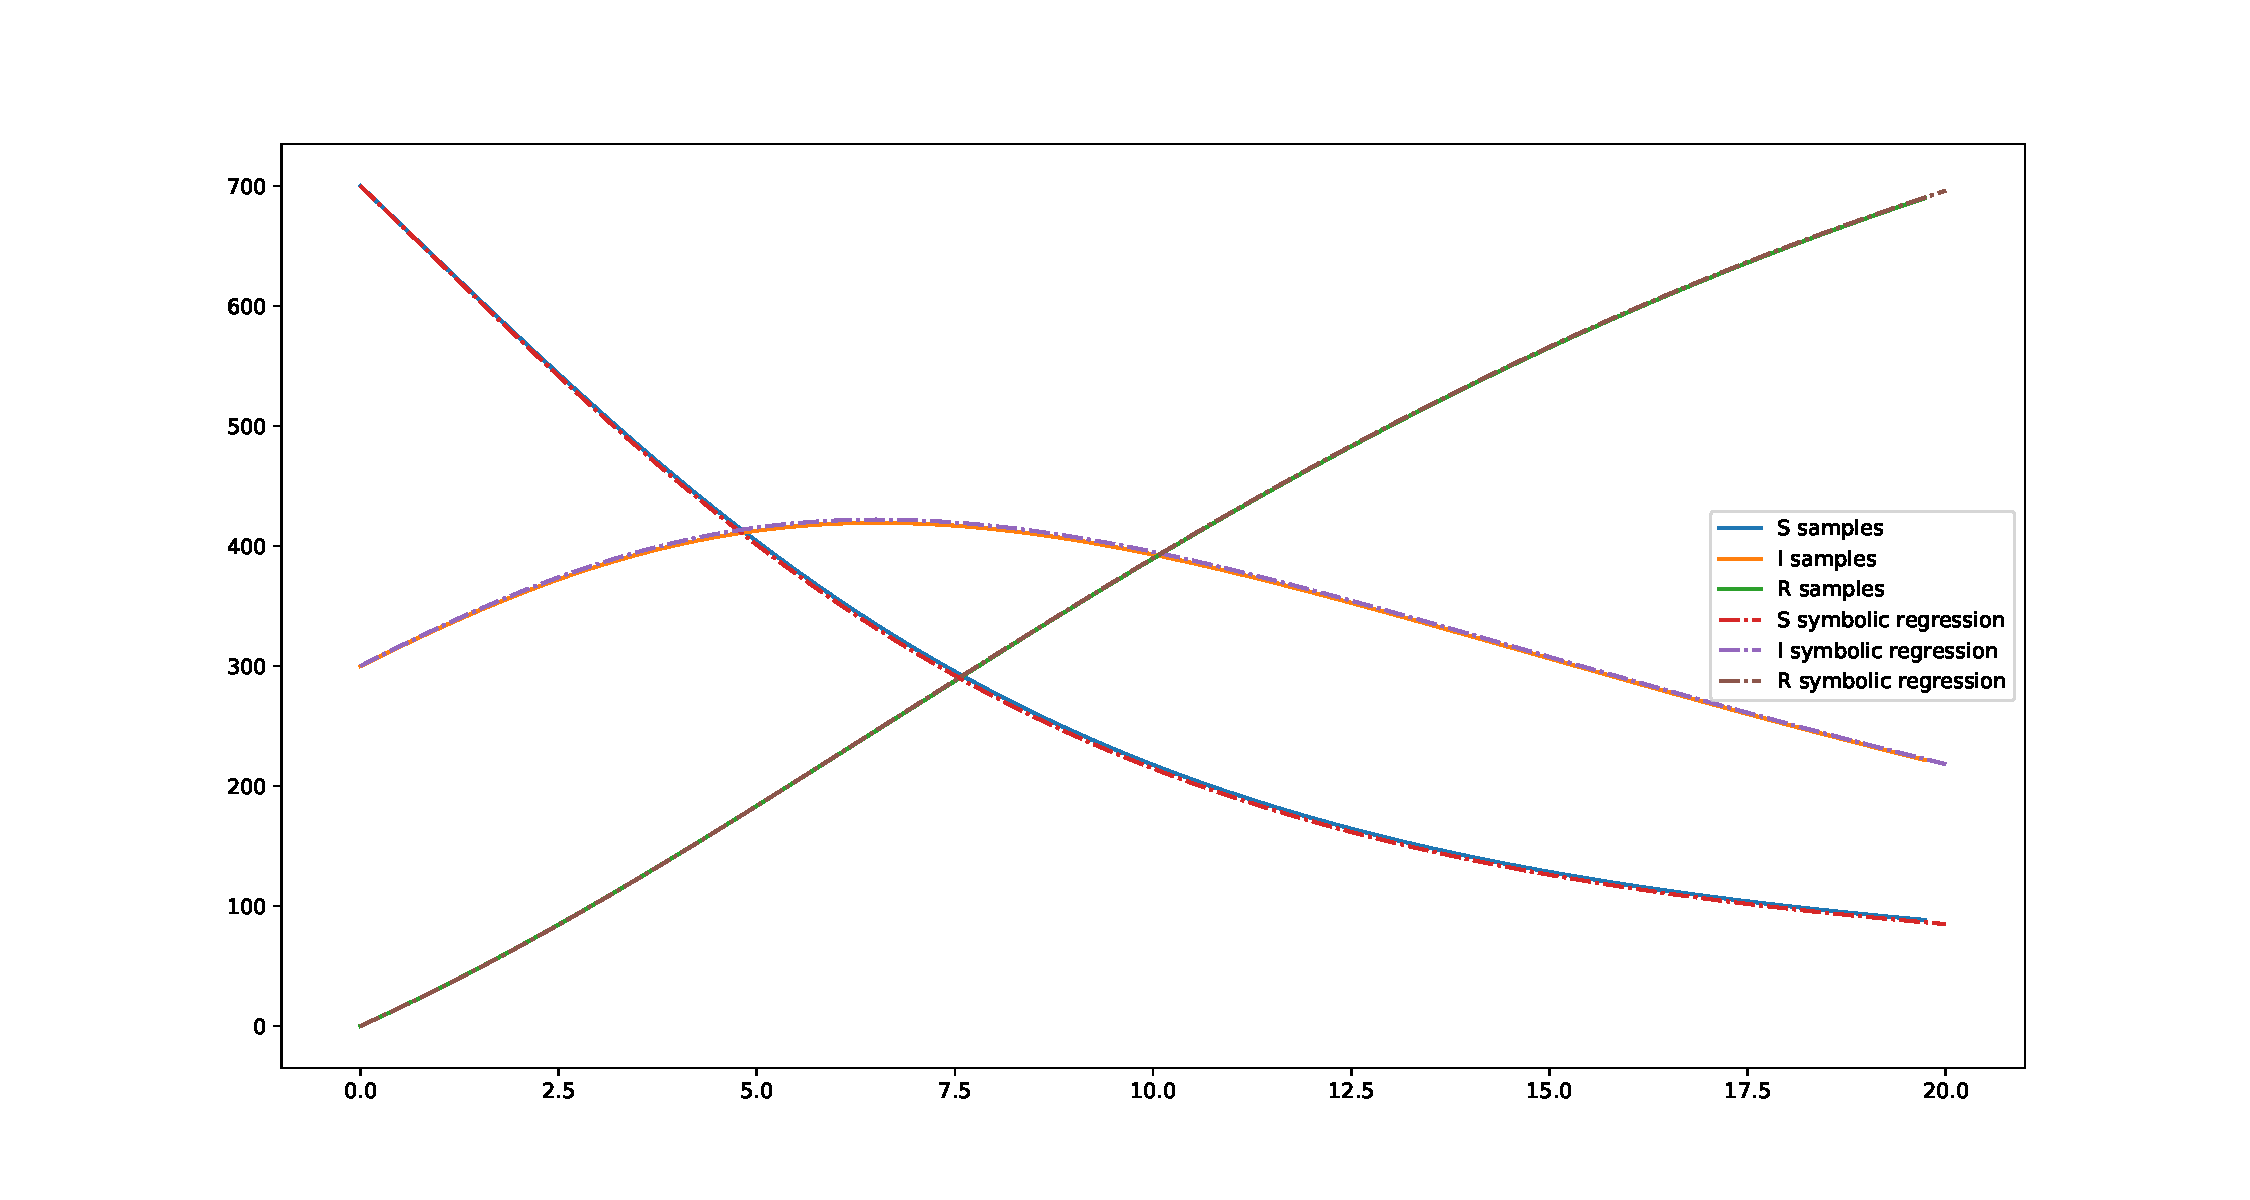
\includegraphics[width=\textwidth]{"figures/final_plot_SIR_0.0.pdf"}
    \caption{Modelo resultante utilizando datos generados a partir del modelo SIR con ruido máximo de 0\%.}
    \label{fig:final_plot_SIR_0.0}
\end{figure}

\begin{figure}[h]
    \centering
    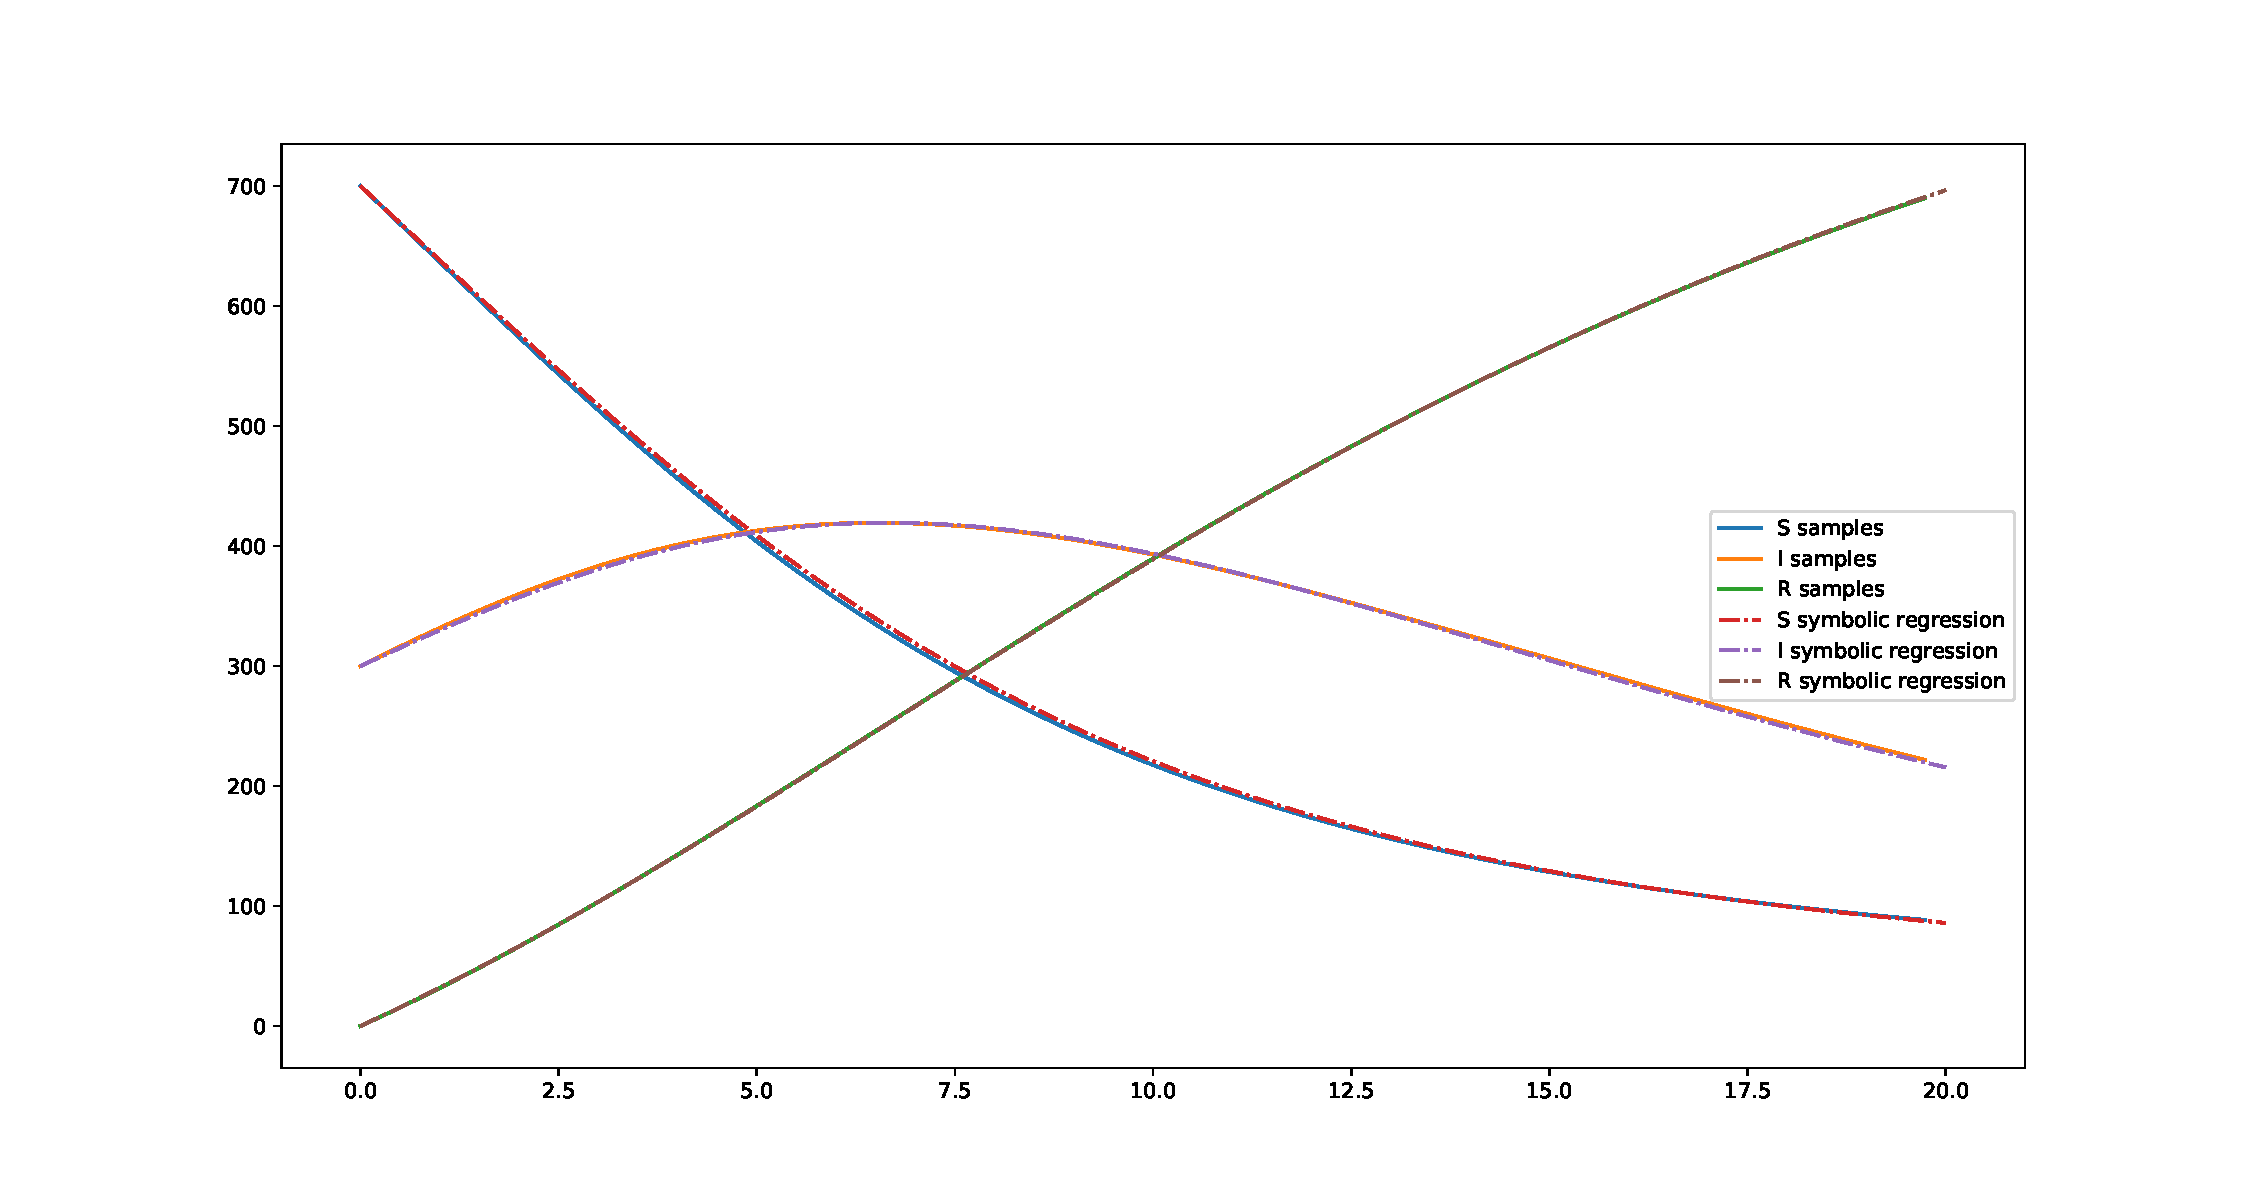
\includegraphics[width=\textwidth]{"figures/final_plot_SIR_0.05.pdf"}
    \caption{Modelo resultante utilizando datos generados a partir del modelo SIR con ruido máximo de 5\%.}
    \label{fig:final_plot_SIR_0.05}
\end{figure}

\begin{figure}[h]
    \centering
    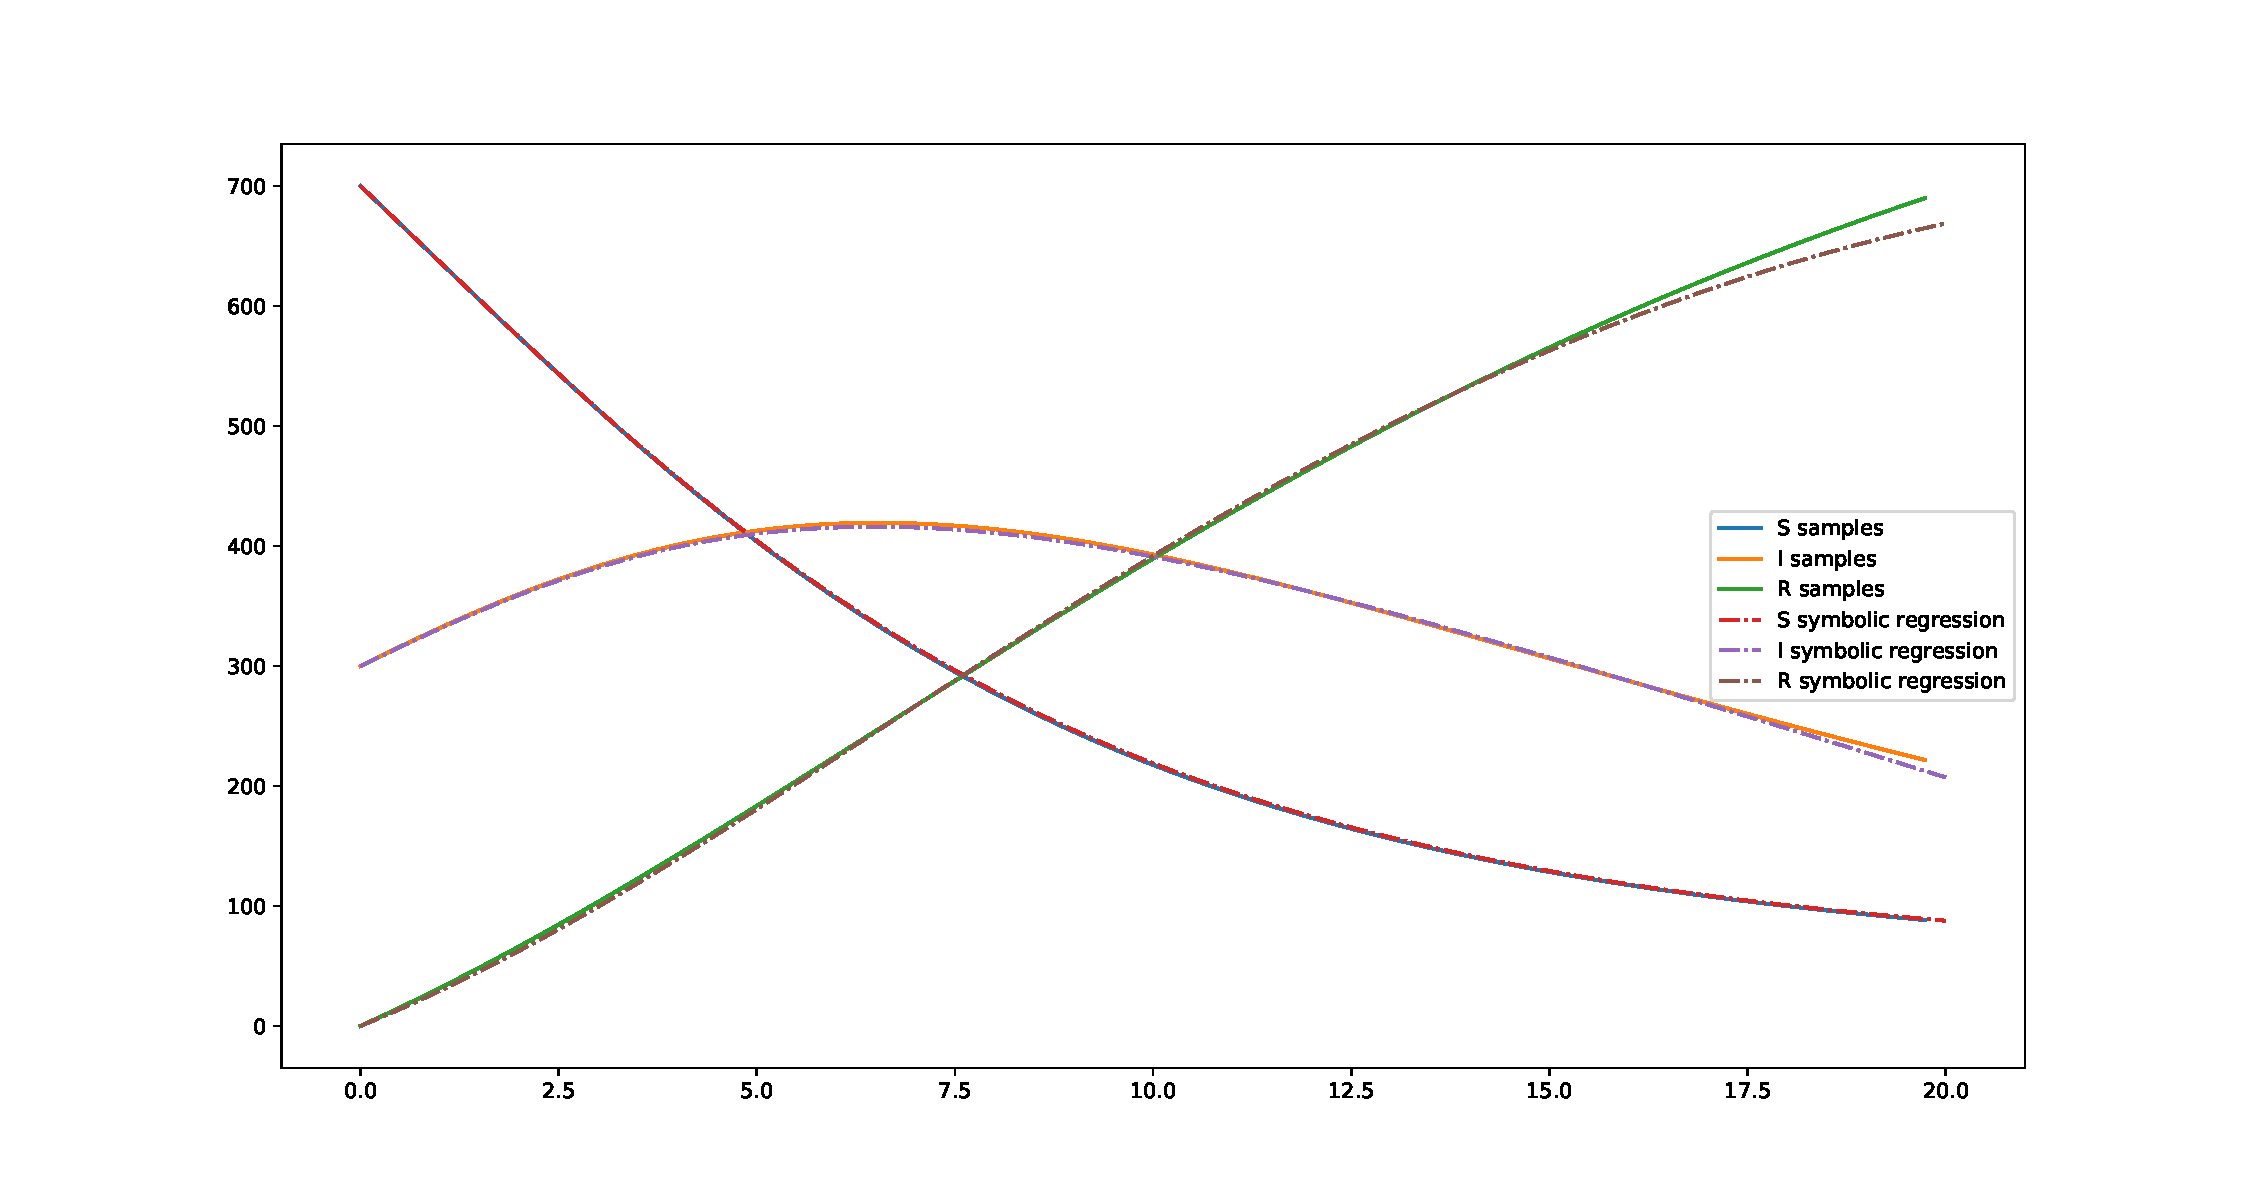
\includegraphics[width=\textwidth]{"figures/final_plot_SIR_0.1.pdf"}
    \caption{Modelo resultante utilizando datos generados a partir del modelo SIR con ruido máximo de 10\%.}
    \label{fig:final_plot_SIR_0.1}
\end{figure}

Si en lugar de utilizar como aproximación el método de diferencias finitas cuando los datos no poseen ruido, se utiliza el sistema original de SIR, se obtiene que la media del valor de la función de ajuste a lo largo de las 30 ejecuciones del experimento es $7.02137e-05$. El valor máximo de la función de ajuste alcanzado fue de $ 0.00116$ y el mínimo de $1.19509e-15$, en este último la regresión simbólica obtuvo exactamente el sistema utilizado para generar los datos.

A continuación se muestra el experimento realizado a partir de la generación de datos utilizando el sistema SIRD.

\subsection{SIRD}

El modelo SIRD es un sistema similar al SIR pero que introduce como dato la cantidad de personas fallecidas $D$ \cite{bailey1975mathematical}. Al modelo SIRD mencionado en \cite{bailey1975mathematical} se le realizó una modificación al añadir un parámetro representando la cantidad de personas que pasan a ser susceptibles en cada instante de tiempo. El sistema se define como:

\begin{align*}
    S' & = a - b (\frac{S I}{S + I + R})         \\
    I' & = b (\frac{S I}{S + I + R}) - c I - d I \\
    R' & = c I                                   \\
    D' & = d I,
\end{align*}

donde $a$ representa la cantidad de personas que pasan a ser susceptibles, $b$ es el índice de contagio de la enfermedad, $c$ es el índice de recuperación y $d$ es el índice de muerte a causa de la enfermedad.

Se utilizaron como valores de los parámetros $a = 250$, $b = 0.5$, $c = 0.1$ y $d = 0.2$ con punto inicial $(7000, 3000, 0, 0)$ y se integró en el intervalo $0 \leq t \leq 20$ para obtener los datos que aparecen en la figura \ref{fig:SIRD}. Del conjunto de puntos se seleccionaron 300 muestras como datos para el método de regresión simbólica.

\begin{figure}[h]
    \centering
    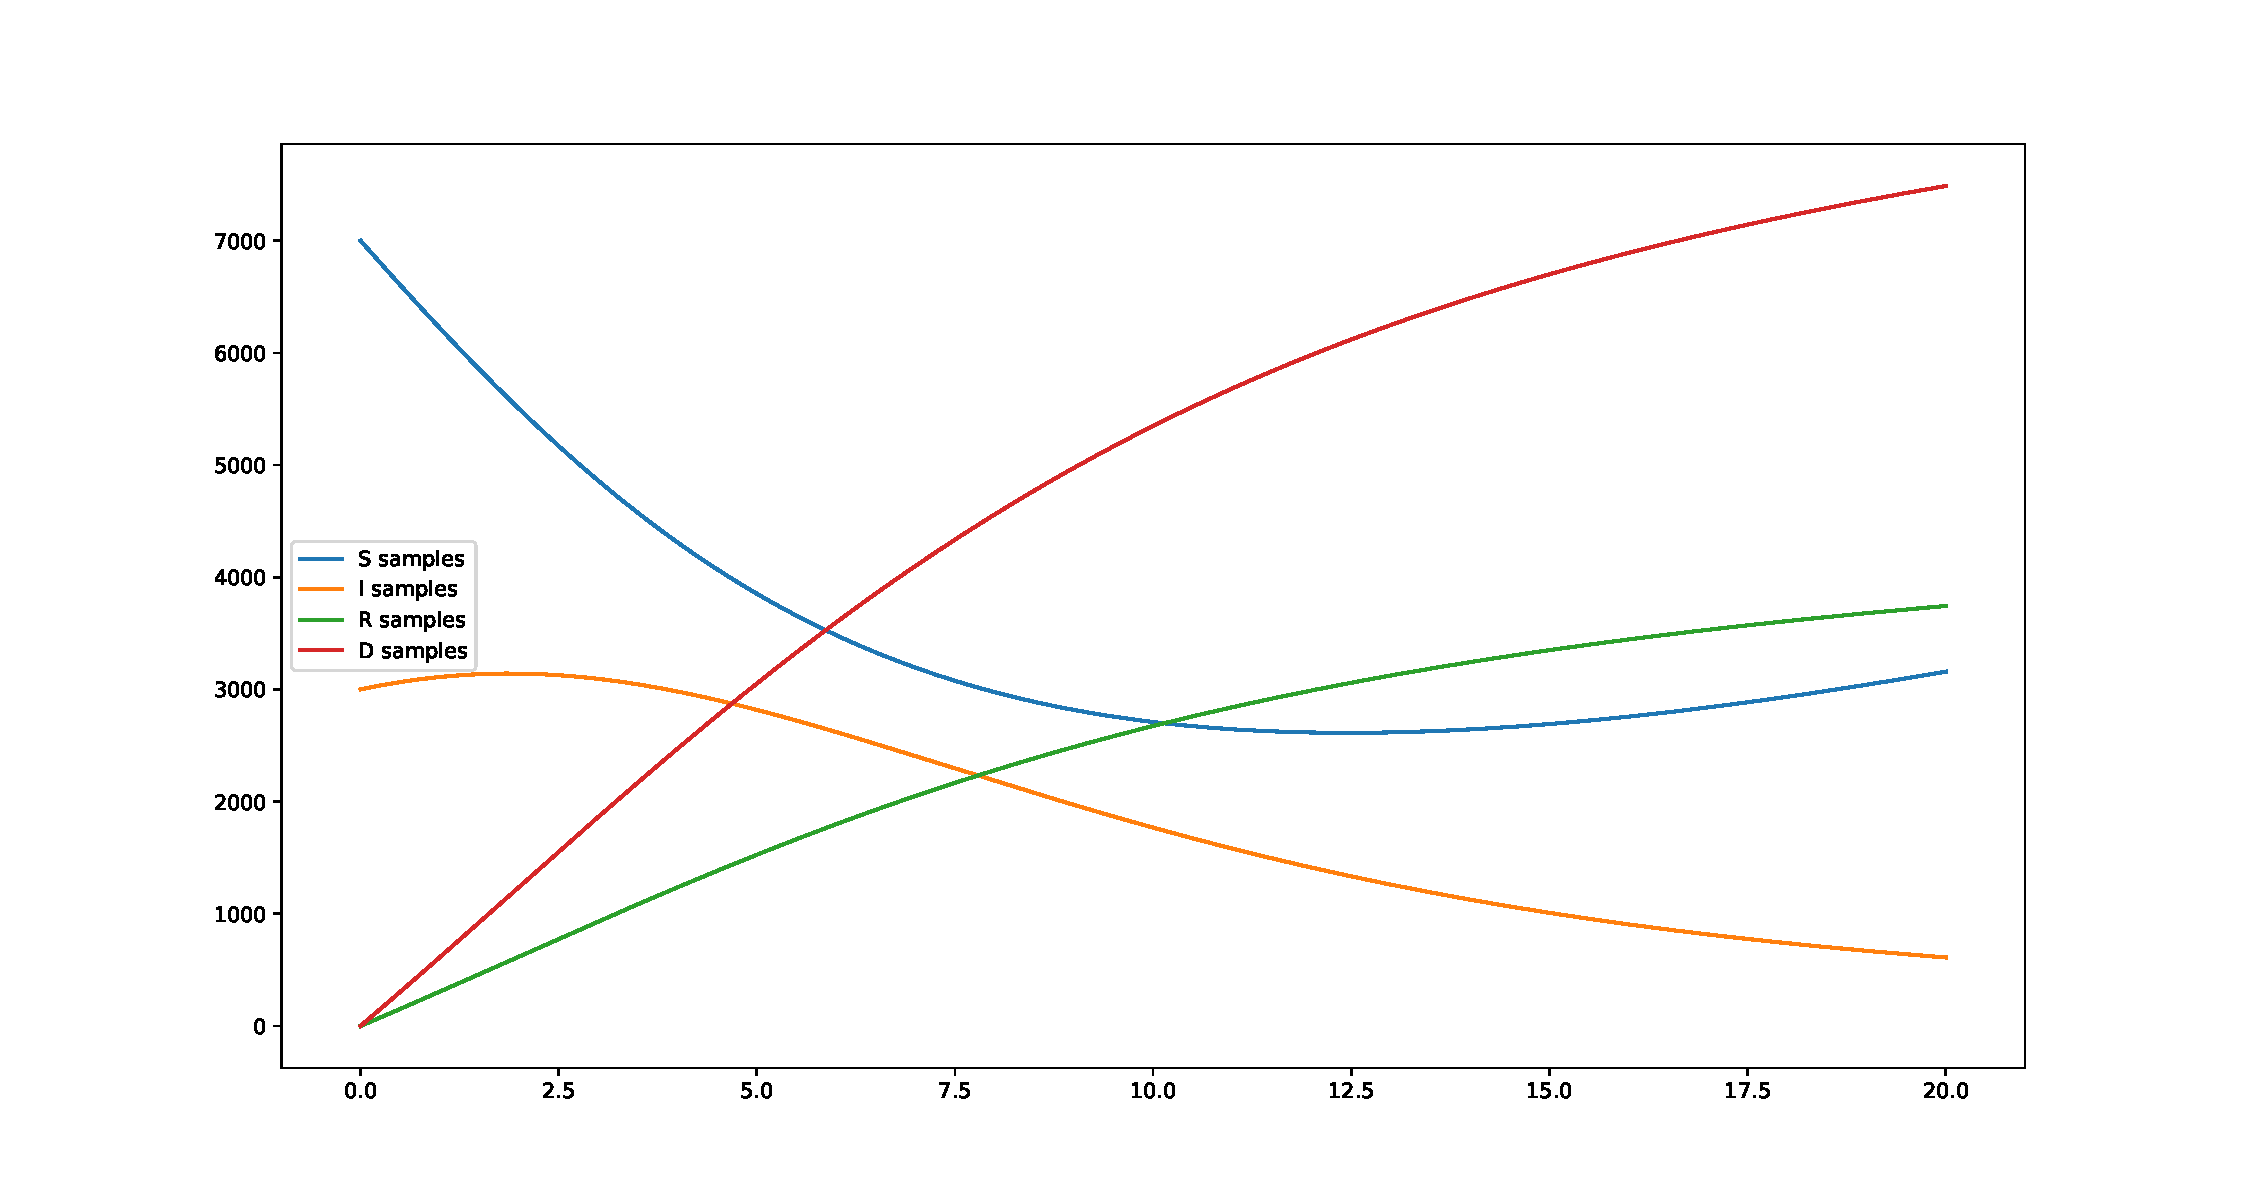
\includegraphics[width=\textwidth]{"figures/SIRD.pdf"}
    \caption{modelo SIRD con $a = 250$, $b = 0.5$, $c = 0.1$ y $d = 0.2$.}
    \label{fig:SIRD}
\end{figure}

Los resultados que se obtienen durante las 30 ejecuciones del experimento, utilizando solamente en cada ecuación las variables permitidas según el modelo y además se agrega como varible $N=S + I + R$, aparecen en la tabla \ref{table:experiment_SIRD} de la página \pageref{table:experiment_SIRD}. Si se permite cualquier variable del modelo en cualquier ecuación del sistema se obtienen los datos que aparecen en la tabla \ref{table:experiment_SIRD_all} de la página \pageref{table:experiment_SIRD_all}.

\begin{table}[!h]
    \centering
    \caption{Resultados que se obtienen en el modelo SIRD restringiendo las variables que aparecen en cada ecuación.}
    \begin{tabular}{|c|c|c|c|}
        \hline
               & \textbf{ruido de 0\%} & \textbf{ruido de 5\%} & \textbf{ruido de 10\%} \\
        \hline
        media  & 47.66074              & 90.64233              & 244.82477              \\
        \hline
        mínimo & 0.51207               & 10.05468              & 18.63161               \\
        \hline
        máximo & 133.55556             & 569.35212             & 2450.05618             \\
        \hline
    \end{tabular}

    \begin{tabular}{|c|c|c|c|c|c|}
        \hline
                             & \textbf{ruido de 0\%} & \textbf{ruido de 5\%} & \textbf{ruido de 10\%} \\
        \hline
        cantidad de sistemas & 22                    & 20                    & 21                     \\
        \hline
        original             & 520.90815             & 894.24332             & 851.17623              \\
        \hline
        original con ruido   & 520.90815             & 917.42578             & 910.64791              \\
        \hline
        spline               & 520.90815             & 894.29561             & 848.03264              \\
        \hline
        otro método          & 596.93643             & 631.63455             & 735.58784              \\
        \hline
    \end{tabular}
    \label{table:experiment_SIRD}
\end{table}

\begin{table}[!h]
    \centering
    \caption{Resultados que se obtienen en el modelo SIRD sin restringir las variables que aparecen en cada ecuación.}
    \begin{tabular}{|c|c|c|c|}
        \hline
               & \textbf{ruido de 0\%} & \textbf{ruido de 5\%} & \textbf{ruido de 10\%} \\
        \hline
        media  & 18.06453              & 109.07249             & 40.10858               \\
        \hline
        mínimo & 0.86131               & 10.14889              & 13.82246               \\
        \hline
        máximo & 49.33228              & 2116.3281             & 193.21428              \\
        \hline
    \end{tabular}

    \begin{tabular}{|c|c|c|c|c|c|}
        \hline
                             & \textbf{ruido de 0\%} & \textbf{ruido de 5\%} & \textbf{ruido de 10\%} \\
        \hline
        cantidad de sistemas & 27                    & 26                    & 24                     \\
        \hline
        original             & 248.31329             & 579.93813             & 652.00833              \\
        \hline
        original con ruido   & 248.31329             & 616.80845             & 743.63415              \\
        \hline
        spline               & 248.31329             & 579.74029             & 644.37875              \\
        \hline
        otro método          & 672.43116             & 674.83326             & 504.66352              \\
        \hline
    \end{tabular}
    \label{table:experiment_SIRD_all}
\end{table}

Durante la realización de los experimentos utilizando el modelo SIRD nunca se obtuvo un sistema igual como resultado de la regresión simbólica, además no se ajustan los datos no importa la cantidad de ruido. El sistema SIRD que se utiliza es el único sistema entre todos los experimentos que posee un término en una ecuación donde aparece un parámetro sin una expresión que lo acompañe.

Los datos que se obtienen de la integración del sistema resultante de la regresión simbólica no se asemejan a los datos de la integración del sistema seleccionado para la realización del experimento, la aparición de ruido afecta aún más el ajuste de los datos.

En las figuras \ref{fig:final_plot_SIRD_0.0} de la página \pageref{fig:final_plot_SIRD_0.0}, \ref{fig:final_plot_SIRD_0.05} de la página \pageref{fig:final_plot_SIRD_0.05} y \ref{fig:final_plot_SIRD_0.1} de la página \pageref{fig:final_plot_SIRD_0.1} se pueden ver los datos originales comparados con los datos obtenidos del mejor resultado generado por la regresión simbólica restringiendo las variables que pueden existir en cada ecuación.

\begin{figure}[h]
    \centering
    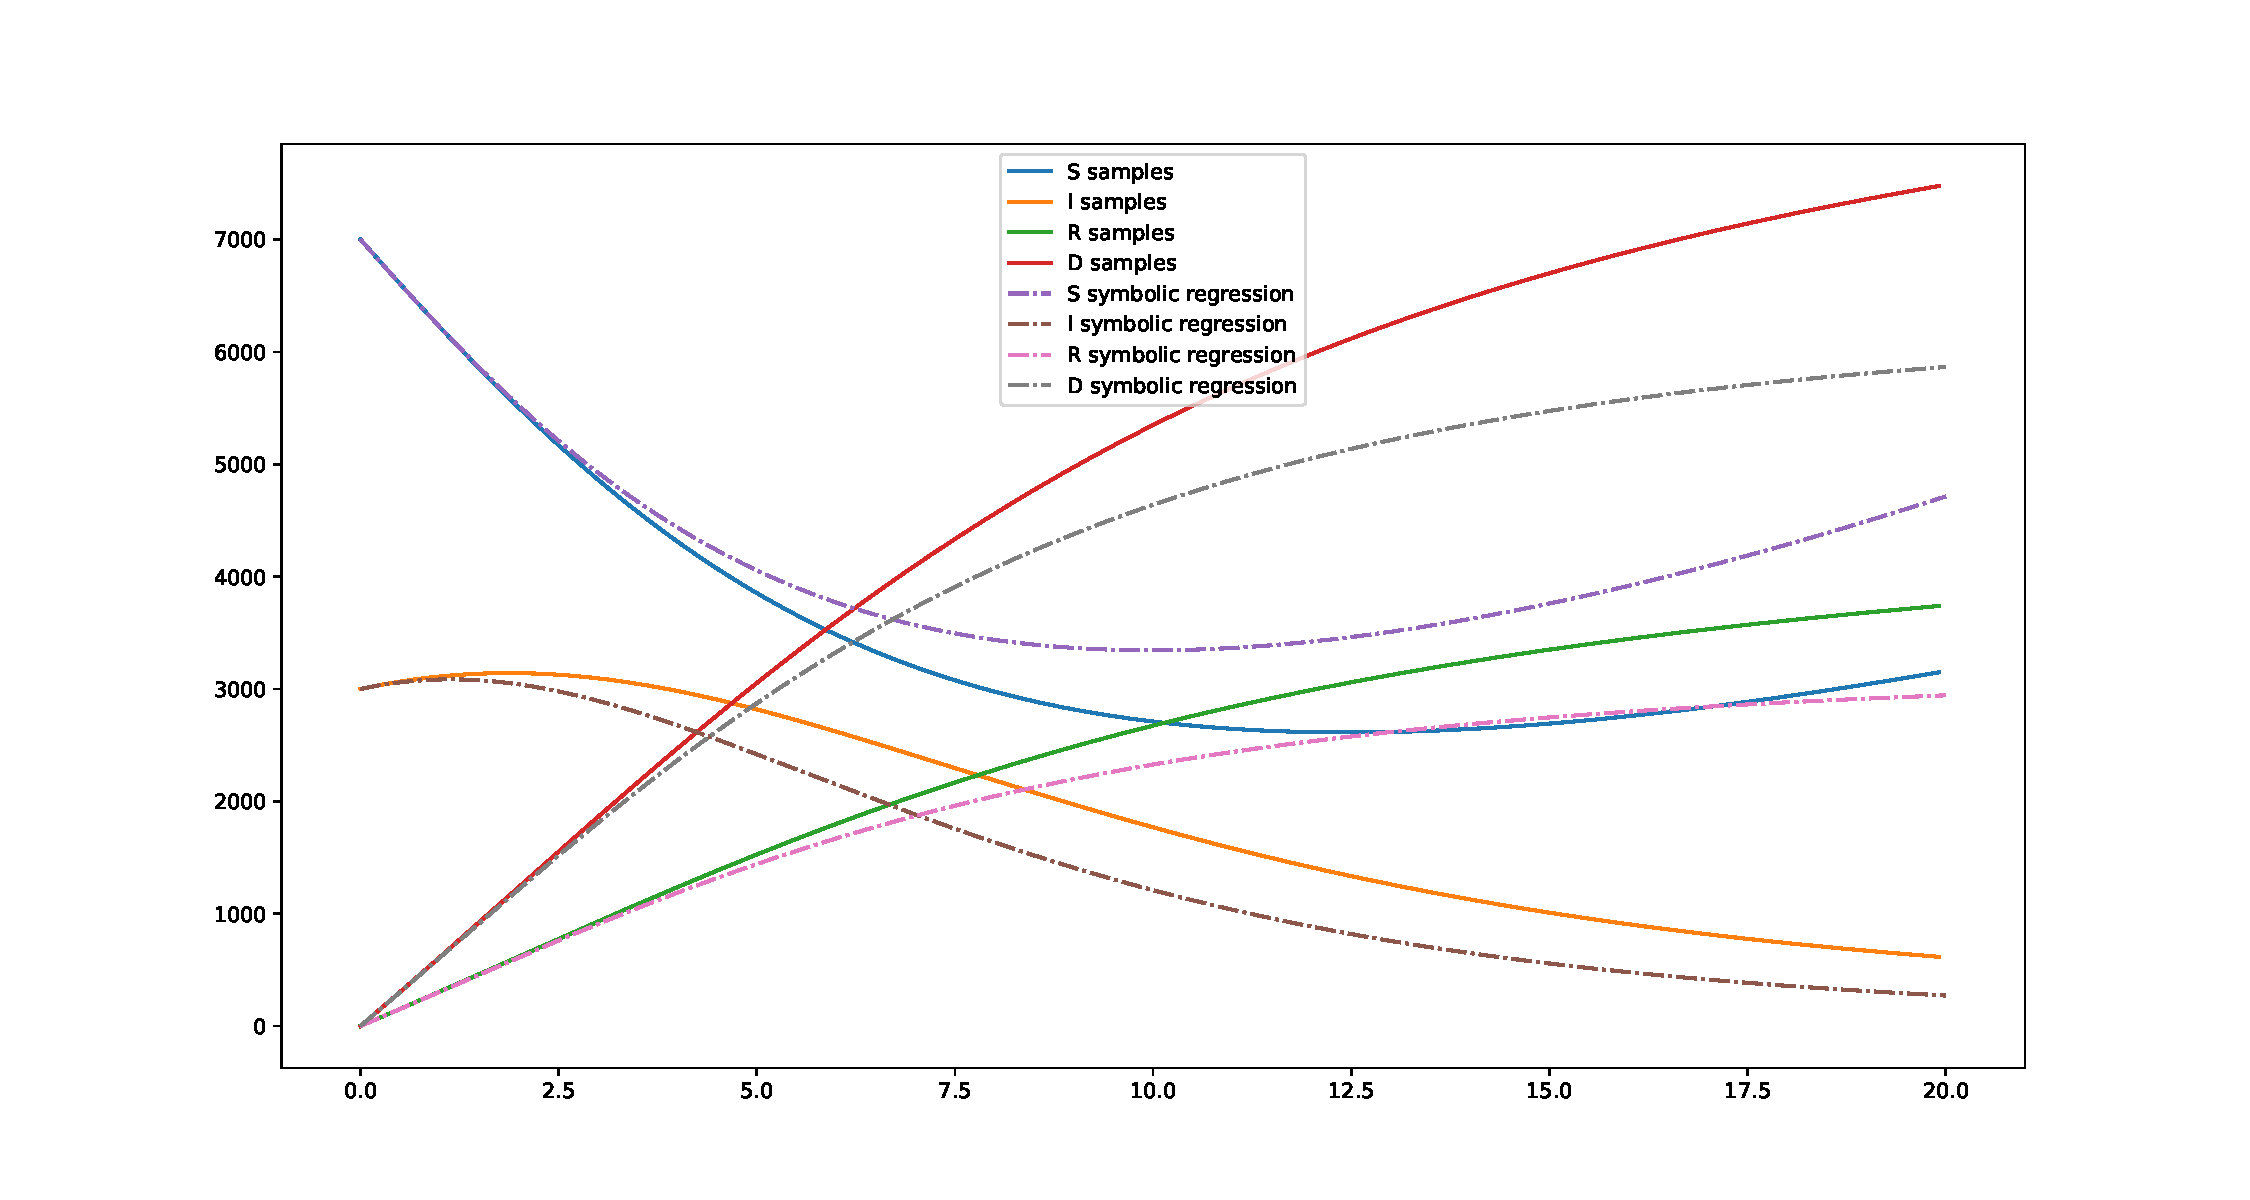
\includegraphics[width=\textwidth]{"figures/final_plot_SIRD_0.0.pdf"}
    \caption{Modelo resultante utilizando datos generados a partir del modelo SIRD con ruido máximo de 0\%.}
    \label{fig:final_plot_SIRD_0.0}
\end{figure}

\begin{figure}[h]
    \centering
    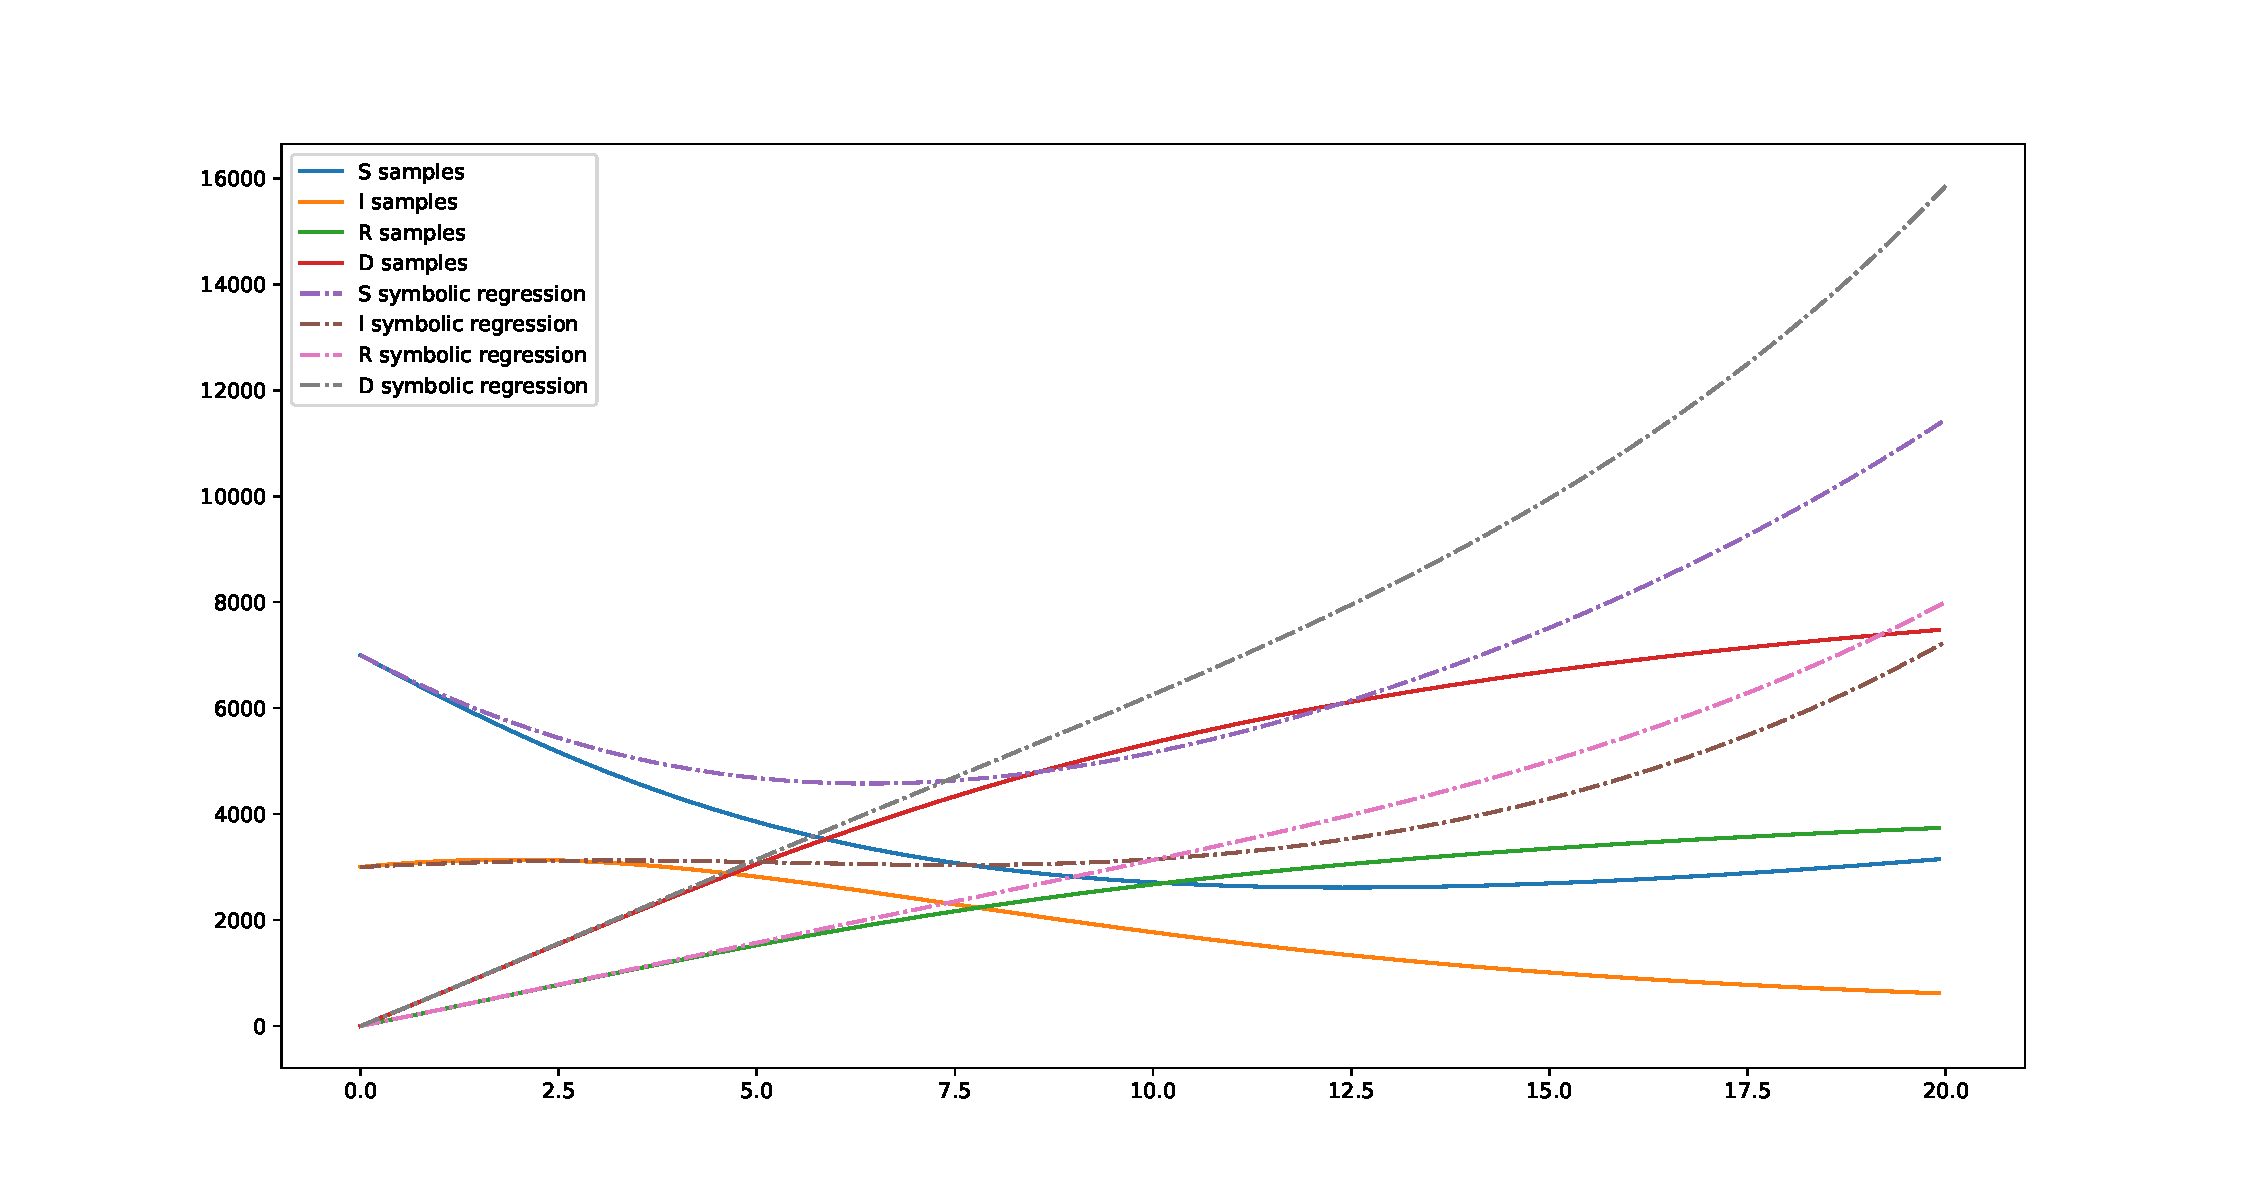
\includegraphics[width=\textwidth]{"figures/final_plot_SIRD_0.05.pdf"}
    \caption{Modelo resultante utilizando datos generados a partir del modelo SIRD con ruido máximo de 5\%.}
    \label{fig:final_plot_SIRD_0.05}
\end{figure}

\begin{figure}[h]
    \centering
    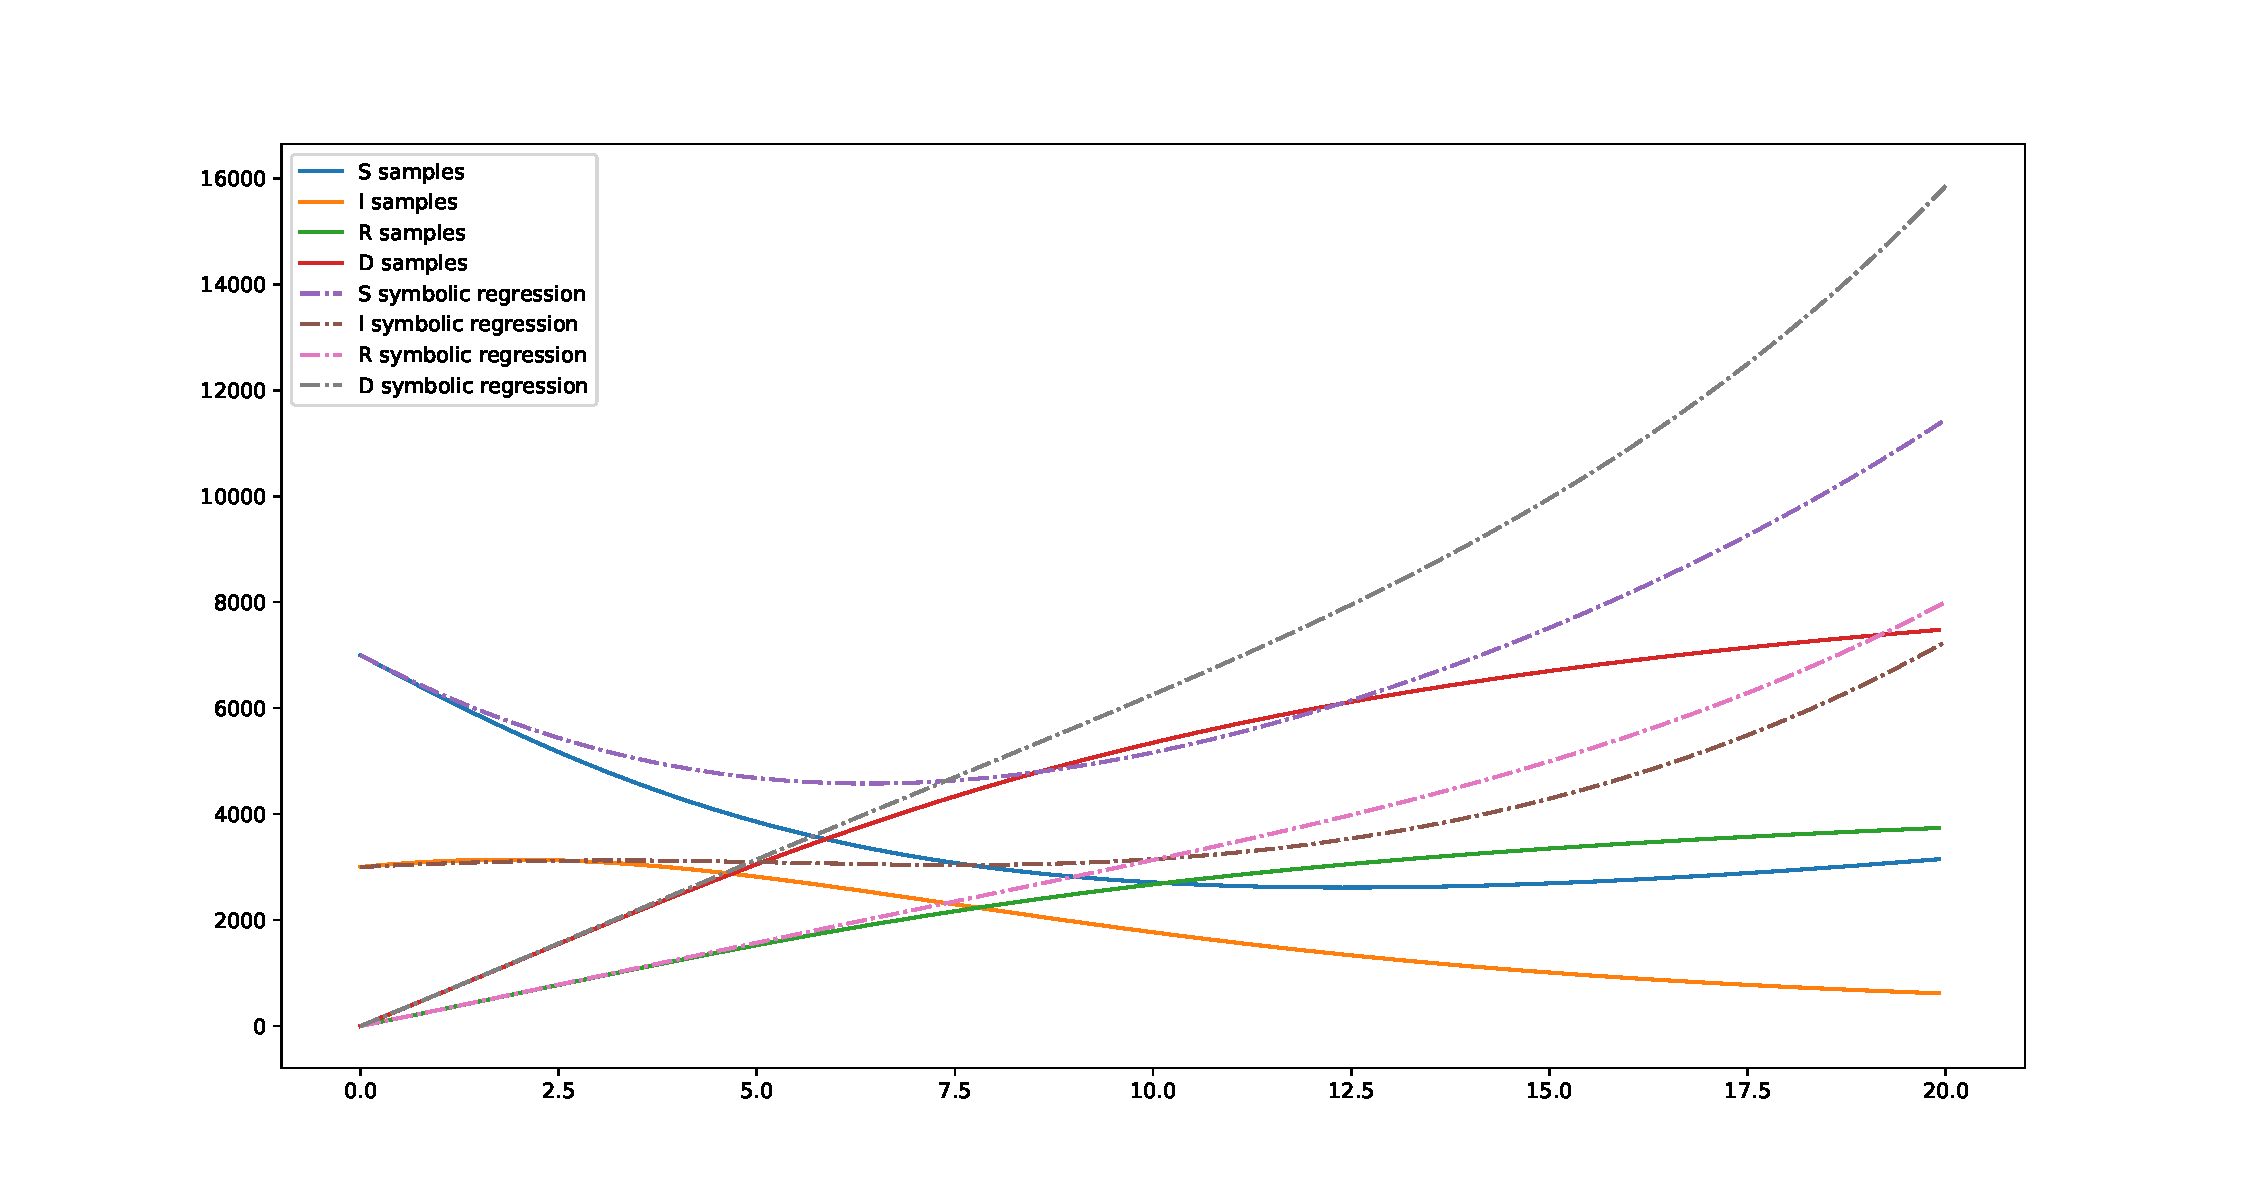
\includegraphics[width=\textwidth]{"figures/final_plot_SIRD_0.1.pdf"}
    \caption{Modelo resultante utilizando datos generados a partir del modelo SIRD con ruido máximo de 10\%.}
    \label{fig:final_plot_SIRD_0.1}
\end{figure}

Si en lugar de utilizar como aproximación el método de diferencias finitas cuando los datos no poseen ruido, se utiliza el sistema original de SIR, se obtiene que la media del valor de la función de ajuste a lo largo de las 30 ejecuciones del experimento es $29.94535$. El valor máximo de la función de ajuste alcanzado fue de $128.83451$ y el mínimo de $2.25834e-14$, en este último la regresión simbólica obtuvo exactamente el sistema utilizado para generar los datos.

A continuación se muestra el experimento realizado a partir de la generación de datos utilizando el sistema SIQRD.

\subsection{SIQRD}

El modelo SIQRD añade al modelo SIRD la posibilidad de aislamiento de una persona, denotado por $Q$, esto modela la situación en que una persona se aisle para no contagiarse o no contagiar a otros \cite{molter2021mathematical}. El sistema se define como:

\begin{align*}
    S' & = -\beta (\frac{S I}{S + I + Q + R + D}) - \alpha S + \delta Q \\
    I' & = \beta (\frac{S I}{S + I + Q + R + D}) - \gamma I - \mu I     \\
    Q' & = \alpha S - \delta Q                                          \\
    R' & = \gamma I                                                     \\
    D' & = \mu I,
\end{align*}

donde $\alpha$ indica la relación con que una persona susceptible es enviada a aislamiento, $\beta$ es el índice de transmisión, $\delta$ indica la relación con que una persona en aislamiento social regresa al grupo de susceptibles, $\gamma$ indica el índice de recuperación y $\mu$ el índice de muerte a causa de la enfermedad.

Se utilizaron como valores de los parámetros $\alpha = 0.2$, $\beta = 0.9$, $\delta = 0.1$, $\gamma = 0.1$ y $\mu = 0.05$ con punto inicial $(5000, 3000, 1000, 0, 0)$ y se integró en el intervalo $0 \leq t \leq 20$ para obtener los datos que aparecen en la imagen \ref{fig:SIQRD} de la página \pageref{fig:SIQRD}. Del conjunto de puntos se seleccionaron 300 muestras como datos para el método de regresión simbólica.

\begin{figure}[h]
    \centering
    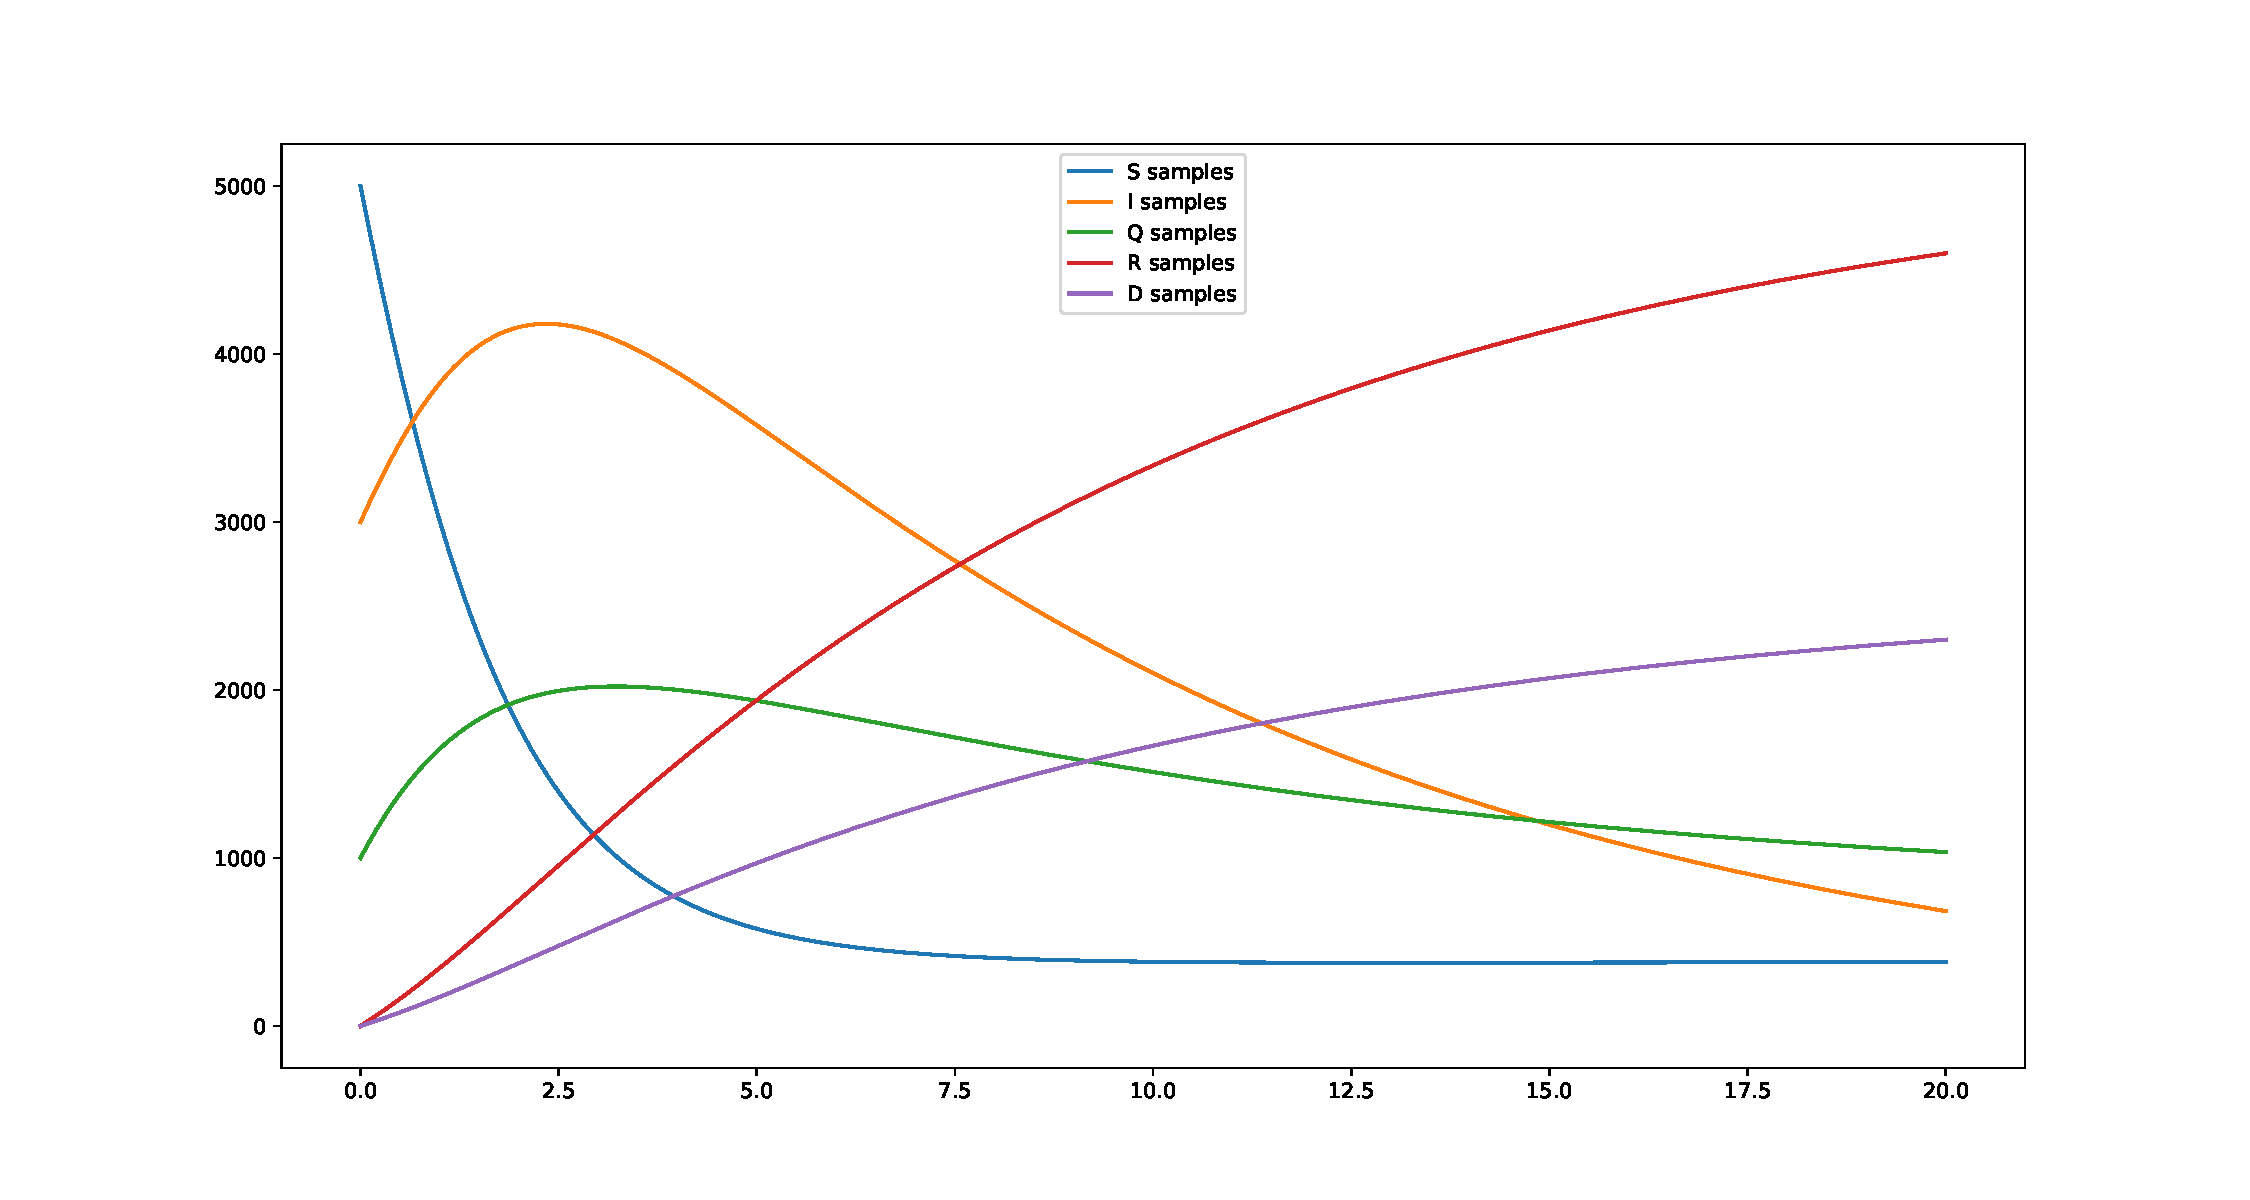
\includegraphics[width=\textwidth]{"figures/SIQRD.pdf"}
    \caption{modelo SIQRD con $\alpha = 0.2$, $\beta = 0.9$, $\delta = 0.1$, $\gamma = 0.1$ y $\mu = 0.05$.}
    \label{fig:SIQRD}
\end{figure}

Los resultados que se obtienen durante las 30 ejecuciones del experimento, utilizando solamente en cada ecuación las variables permitidas según el modelo y además se agrega como varible $N=S + I + Q + R + D$, aparecen en la tabla \ref{table:experiment_SIQRD} de la página \pageref{table:experiment_SIQRD}. Si se permite cualquier variable del modelo en cualquier ecuación del sistema se obtienen los datos que aparecen en la tabla \ref{table:experiment_SIQRD_all} de la página \pageref{table:experiment_SIQRD_all}.

\begin{table}[!h]
    \centering
    \caption{Resultados que se obtienen en el modelo SIQRD restringiendo las variables que aparecen en cada ecuación.}
    \begin{tabular}{|c|c|c|c|}
        \hline
               & \textbf{ruido de 0\%} & \textbf{ruido de 5\%} & \textbf{ruido de 10\%} \\
        \hline
        media  & 7.47098               & 35.17738              & 38.70691               \\
        \hline
        mínimo & 1.35941               & 7.96579               & 12.25428               \\
        \hline
        máximo & 49.24056              & 99.18317              & 197.34403              \\
        \hline
    \end{tabular}

    \begin{tabular}{|c|c|c|c|c|c|}
        \hline
                             & \textbf{ruido de 0\%} & \textbf{ruido de 5\%} & \textbf{ruido de 10\%} \\
        \hline
        cantidad de sistemas & 29                    & 22                    & 22                     \\
        \hline
        original             & 76.49518              & 517.5006              & 338.54534              \\
        \hline
        original con ruido   & 76.49518              & 536.1417              & 395.29378              \\
        \hline
        spline               & 76.49518              & 515.51251             & 338.39969              \\
        \hline
        otro método          & 698.3556              & 919.78558             & 747.2666               \\
        \hline
    \end{tabular}
    \label{table:experiment_SIQRD}
\end{table}

\begin{table}[!h]
    \centering
    \caption{Resultados que se obtienen en el modelo SIQRD sin restringir las variables que aparecen en cada ecuación.}
    \begin{tabular}{|c|c|c|c|}
        \hline
               & \textbf{ruido de 0\%} & \textbf{ruido de 5\%} & \textbf{ruido de 10\%} \\
        \hline
        media  & 5.00116               & 34.76361              & 33.05852               \\
        \hline
        mínimo & 2.43638               & 8.78968               & 13.28306               \\
        \hline
        máximo & 7.84816               & 80.32846              & 83.9451                \\
        \hline
    \end{tabular}

    \begin{tabular}{|c|c|c|c|c|c|}
        \hline
                             & \textbf{ruido de 0\%} & \textbf{ruido de 5\%} & \textbf{ruido de 10\%} \\
        \hline
        cantidad de sistemas & 29                    & 20                    & 19                     \\
        \hline
        original             & 69.88262              & 357.61219             & 259.33185              \\
        \hline
        original con ruido   & 69.88262              & 372.24346             & 312.84906              \\
        \hline
        spline               & 69.88262              & 356.83797             & 253.63394              \\
        \hline
        otro método          & 730.13032             & 901.498               & 735.24475              \\
        \hline
    \end{tabular}
    \label{table:experiment_SIQRD_all}
\end{table}

Con este experimento se obtiene que los sistemas generados por la regresión simbólica ajustan los datos mientras estos no posean ruido. Los datos que se obtienen de la integración del sistema resultante de la regresión simbólica se asemejan a los datos de la integración del sistema seleccionado para la realización del experimento pero la aparición de ruido afecta el ajuste de los datos. Los datos que se obtienen de la integración del sistema obtenido a partir de un conjunto de datos con ruido máximo de 5\% obtiene peores resultados que si se utiliza como ruido máximo 10\%. Esto se puede deber a un mal ajuste del parámetro de suavizado utilizado en spline de suavizado.

En las figuras \ref{fig:final_plot_SIQRD_0.0} de la página \pageref{fig:final_plot_SIQRD_0.0}, \ref{fig:final_plot_SIQRD_0.05} de la página \pageref{fig:final_plot_SIQRD_0.05} y \ref{fig:final_plot_SIQRD_0.1} de la página \pageref{fig:final_plot_SIQRD_0.1} se pueden ver los datos originales comparados con los datos obtenidos del mejor resultado generado por la regresión simbólica restringiendo las variables que pueden existir en cada ecuación.

\begin{figure}[h]
    \centering
    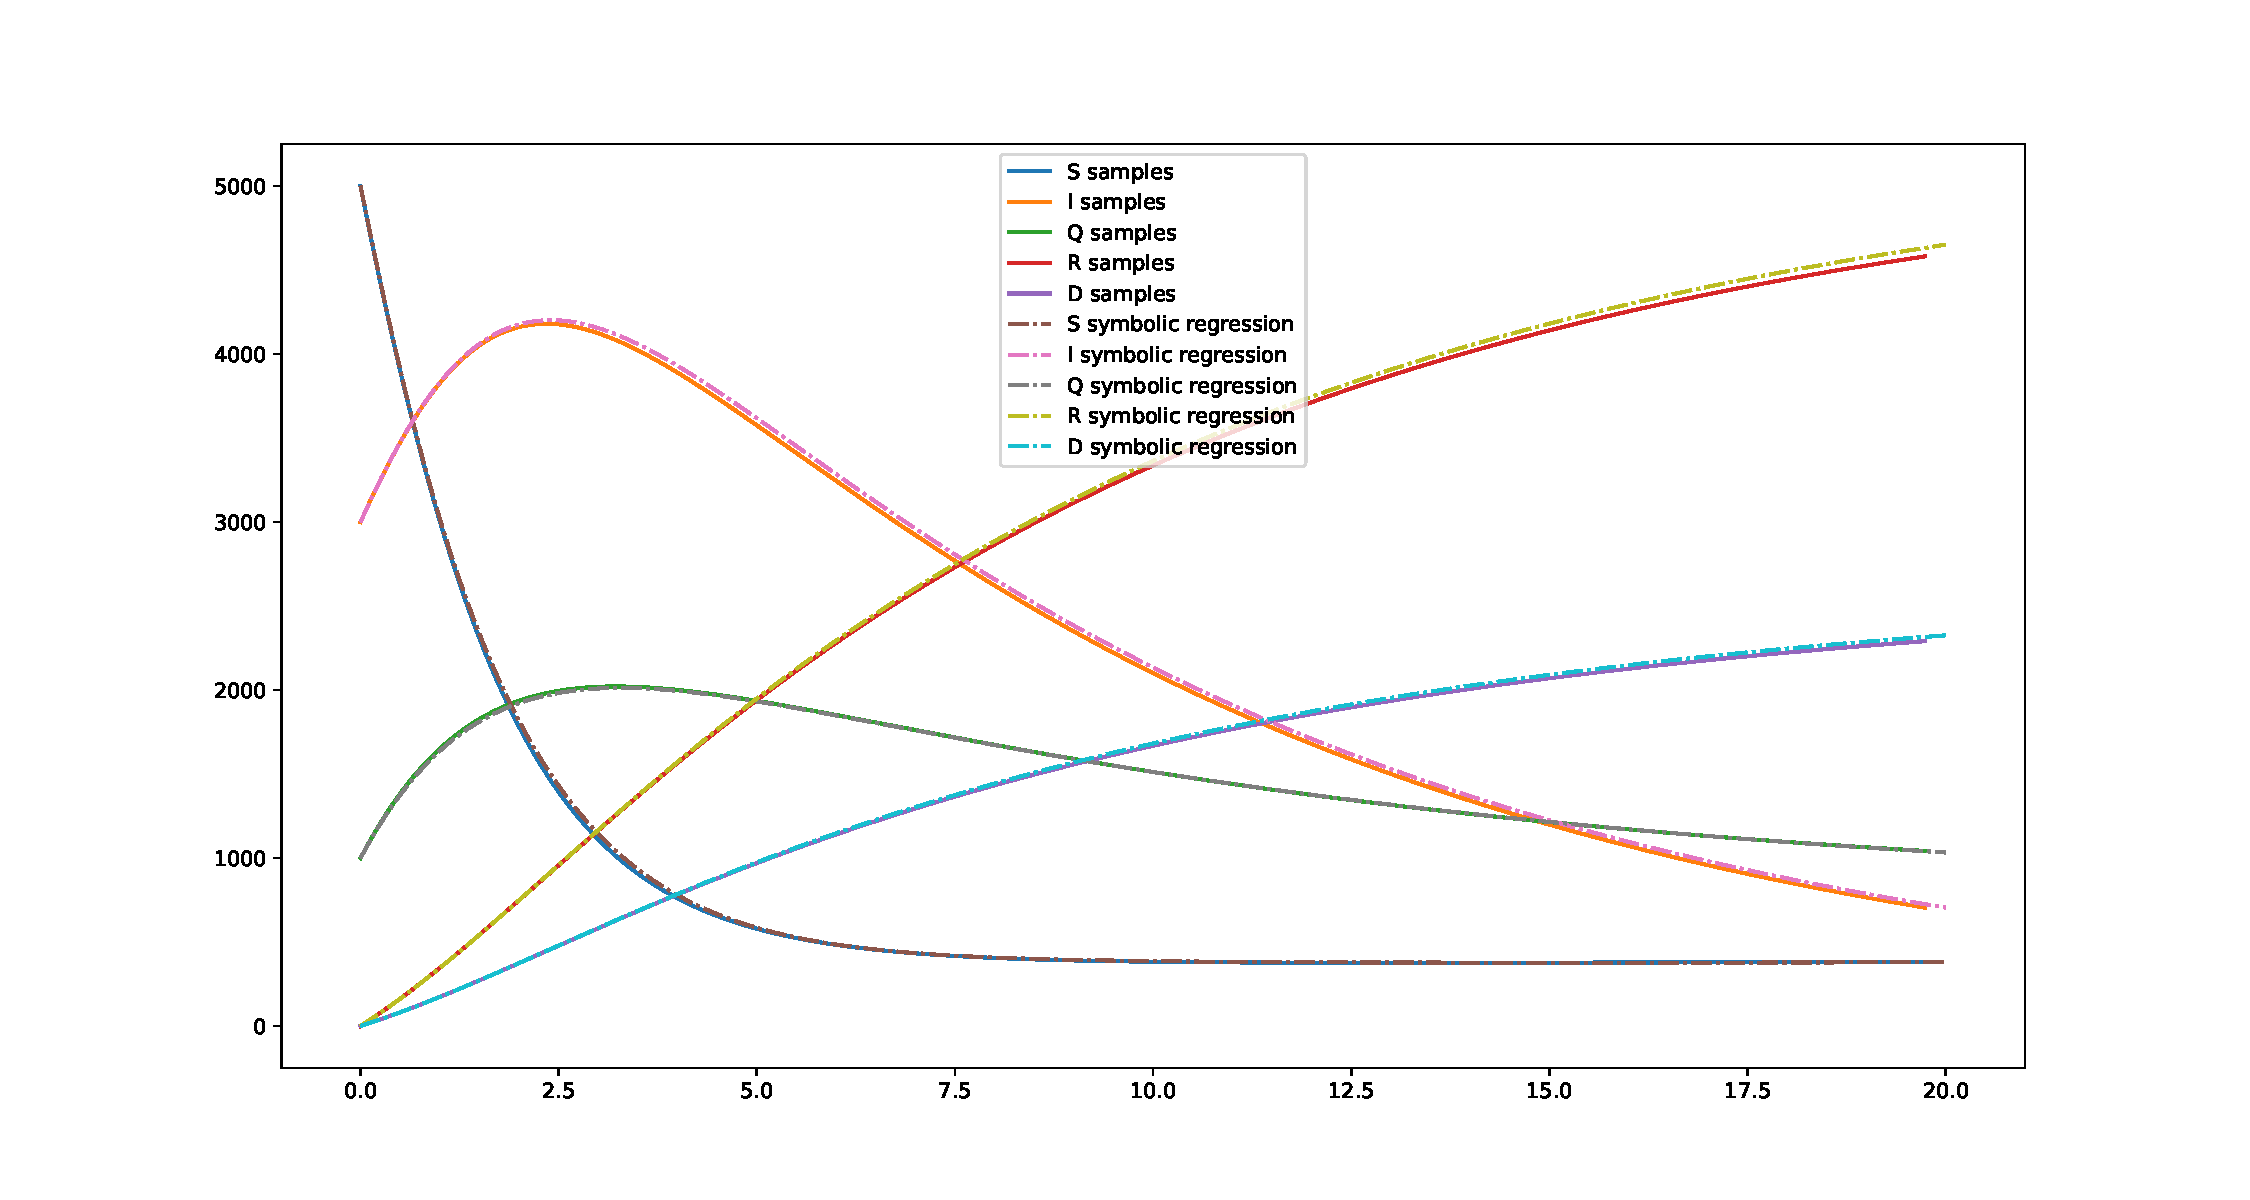
\includegraphics[width=\textwidth]{"figures/final_plot_SIQRD_0.0.pdf"}
    \caption{Modelo resultante utilizando datos generados a partir del modelo SIQRD con ruido máximo de 0\%.}
    \label{fig:final_plot_SIQRD_0.0}
\end{figure}

\begin{figure}[h]
    \centering
    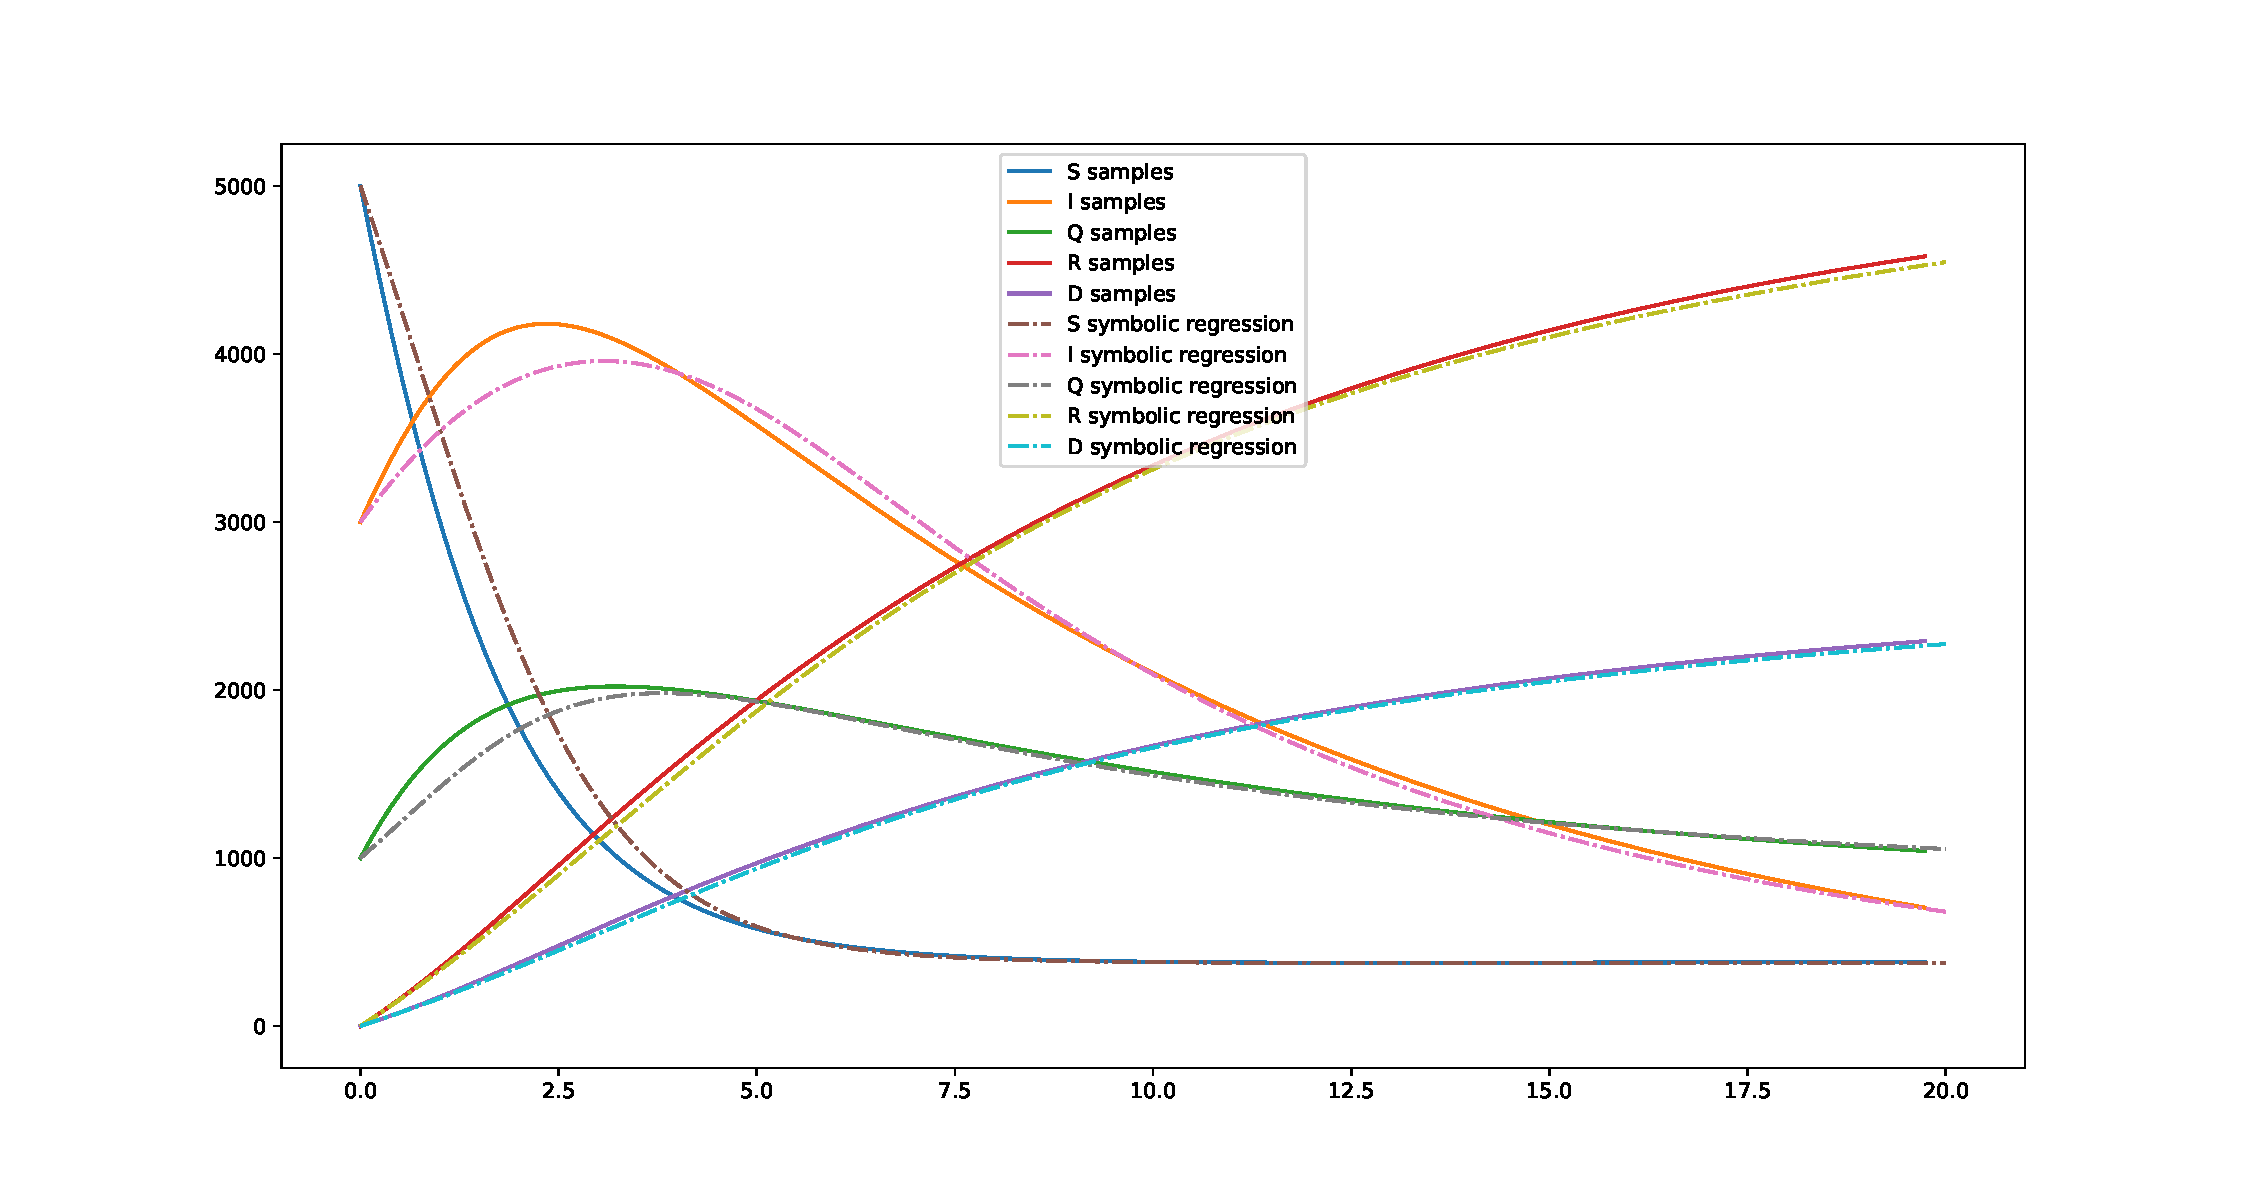
\includegraphics[width=\textwidth]{"figures/final_plot_SIQRD_0.05.pdf"}
    \caption{Modelo resultante utilizando datos generados a partir del modelo SIQRD con ruido máximo de 5\%.}
    \label{fig:final_plot_SIQRD_0.05}
\end{figure}

\begin{figure}[h]
    \centering
    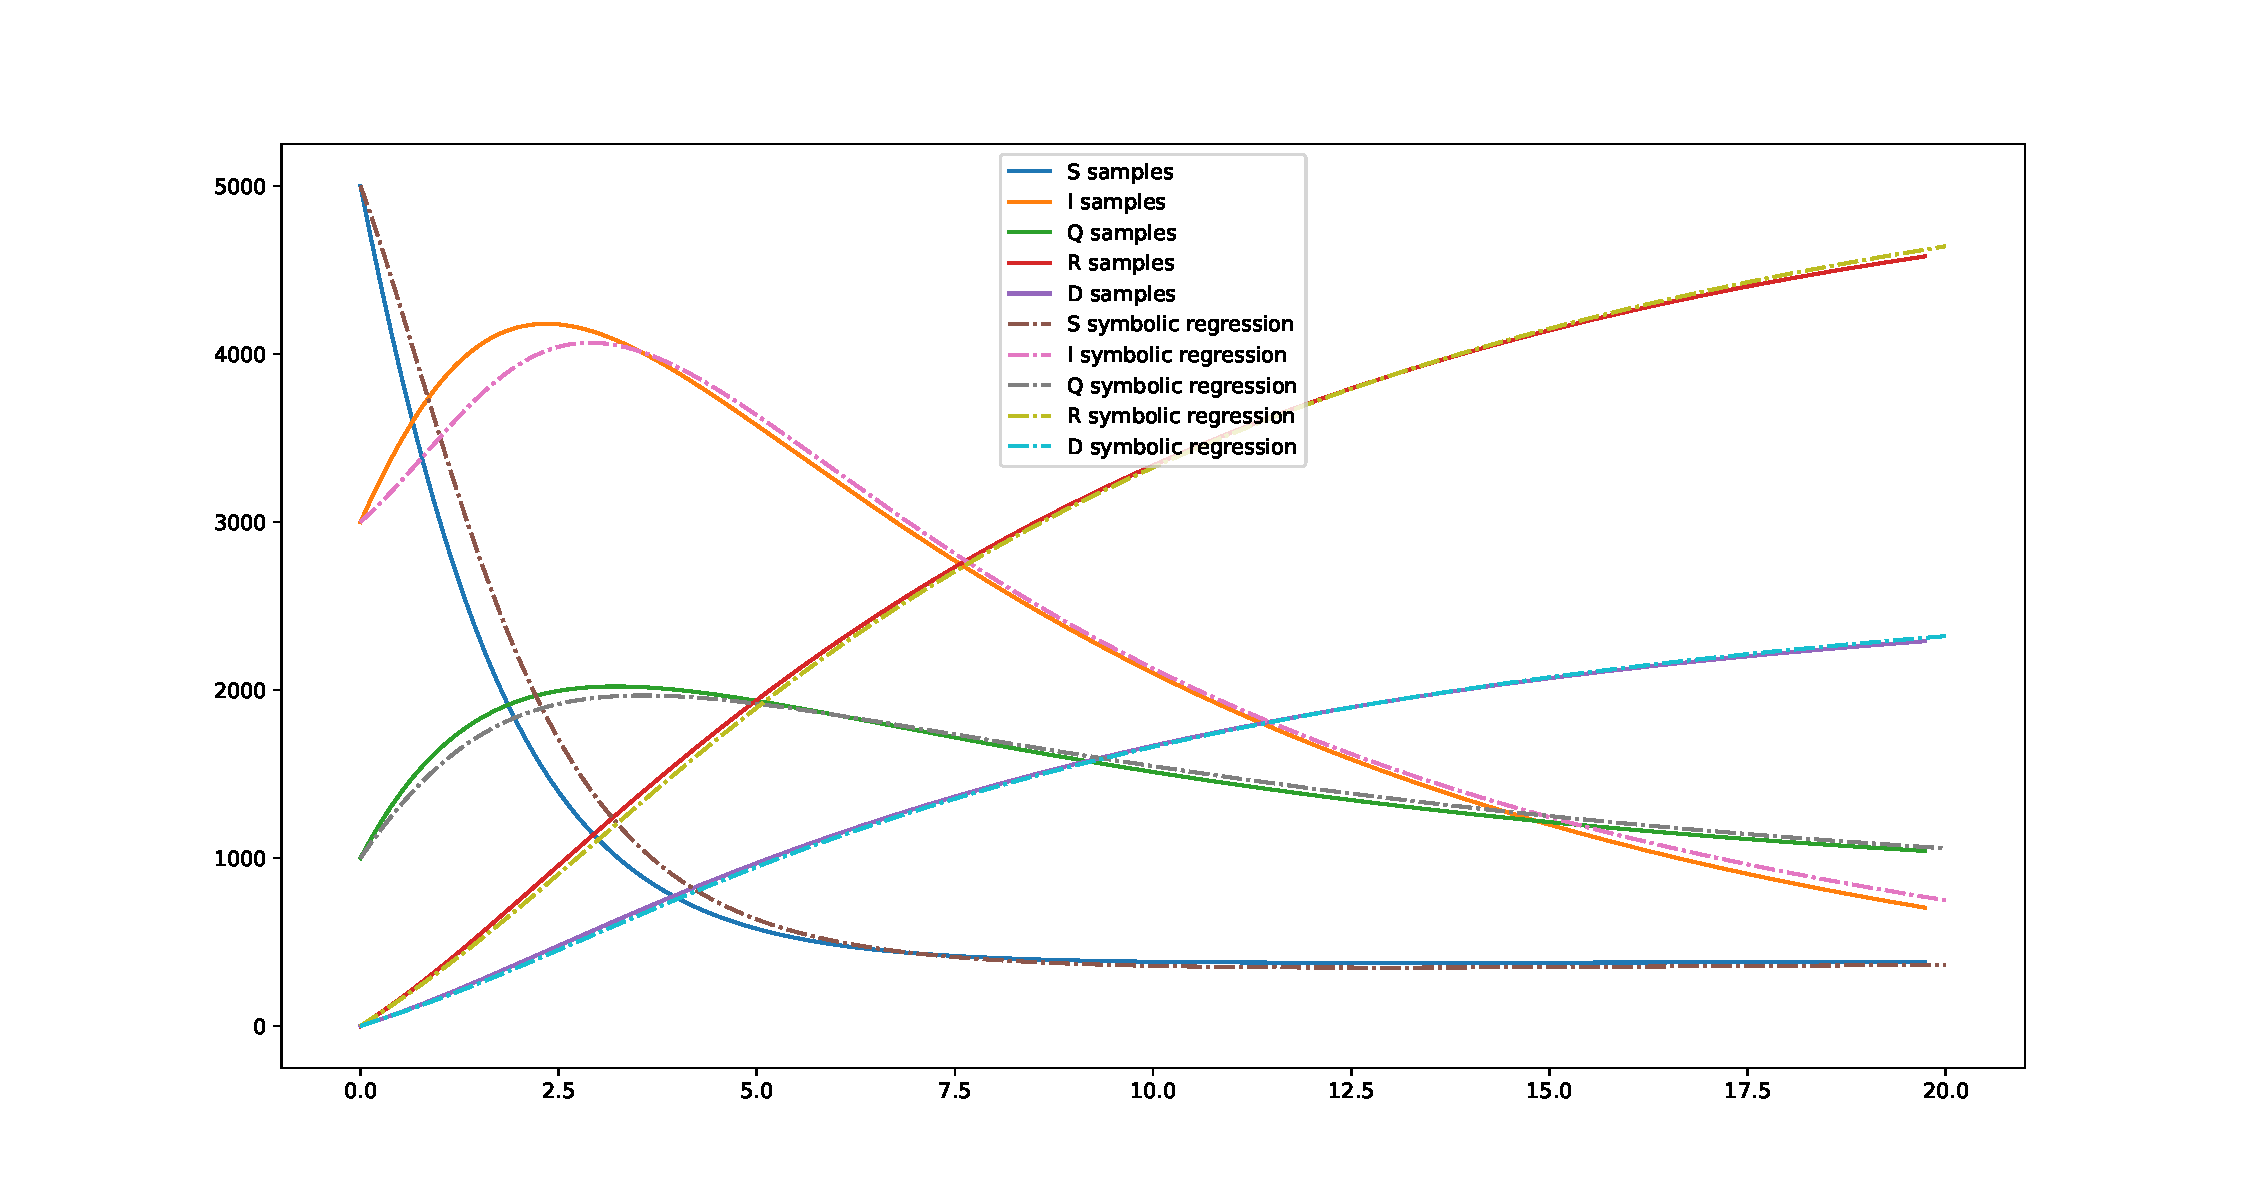
\includegraphics[width=\textwidth]{"figures/final_plot_SIQRD_0.1.pdf"}
    \caption{Modelo resultante utilizando datos generados a partir del modelo SIQRD con ruido máximo de 10\%.}
    \label{fig:final_plot_SIQRD_0.1}
\end{figure}

Si en lugar de utilizar como aproximación el método de diferencias finitas cuando los datos no poseen ruido, se utiliza el sistema original de SIR, se obtiene que la media del valor de la función de ajuste a lo largo de las 30 ejecuciones del experimento es $6.01436$. El valor máximo de la función de ajuste alcanzado fue de $48.48072$ y el mínimo de $1.42392e-14$, en este último la regresión simbólica obtuvo el sistema:

\begin{align*}
    S' & = -0.1 * S -0.1 * S + -0.0001 * (I * S) + 0.1 * Q \\
    I' & = -0.075 * I + 0.0001 * (S * I) -0.075 * I        \\
    Q' & = -0.1 * Q + 0.2 * S                              \\
    R' & = -0.1 * -I                                       \\
    D' & = 0.025 * I + 0.025 * I,
\end{align*}

que es igual al sistema original si se asume $\frac{\beta}{N} = 0.0001$.

A continuación se muestra el experimento realizado a partir de la generación de datos utilizando el sistema SVVEIR.

\subsection{SVVEIR}

El modelo SVVEIR describe un escenario de una posible enfermedad en la sociedad de Bangladesh. En el modelo se plantea un conjunto $S$ de individuos que no se han infectado aún, $V_1$ y $V_2$ son los individuos que han recibido la primera y segunda vacuna, respectivamente. Las personas infectadas pero que aún no han desarrollado síntomas se definen como expuestos y se encuentran representados por el conjunto $E$. Los parámetros $I$ y $R$ identifican los mismos conjuntos que en el modelo SIR \cite{kuddus2021mathematical}. El sistema se define como:


\begin{align*}
    N    & = S + V_1 + V_2 + E + I + R                                        \\
    S'   & = \mu * N - \beta * \frac{I}{N} * S - n * S - \mu * S + \rho * V_1 \\
    V_1' & = n * S - \rho * V_1 - \sigma * V_1 - \mu * V_1                    \\
    V_2' & = \sigma * V_1 - \omega * V_2 - \mu * V_2                          \\
    E'   & = \beta * I / N * S - \alpha * E - \mu * E                         \\
    I'   & = \alpha * E - \gamma * I - \delta * I - \mu * I                   \\
    R'   & = \gamma * I + \omega * V_2 - \mu * R,
\end{align*}

donde $\alpha$ indica la relación de personas expuestas que pasan a estar infectados, $\beta$ es el índice de transmisión de la enfermedad, $\delta$ es el índice de muerte debido a la enfermedad mientras que $\mu$ es el índice de muerte por causas naturales. El índice de recuperación de la enfermedad se representa mediante el parámetro $\gamma$. El parámetro $n$ muestra el índice de personas susceptibles que reciben la primera dosis de la vacuna y $\rho$ describe la relación de personas con una sola dosis de la vacuna que regresan al grupo de susceptibles. La cantidad de personas que reciben la segunda dosis se refleja en el parámetro $\sigma$ y $\omega$ es el parámetro que muestra la relación de personas con dos dosis de la vacuna que pasan a recuperados.

Se utilizaron como valores de los parámetros $\alpha = 0.1$, $\beta = 0.7$, $\delta = 0.0005$, $\gamma = 0.05$, $\mu = 0.01$, $n = 0.2$, $\rho = 0.01$, $\omega = 0.05$ y $\sigma = 0.2$ con punto inicial $(5000, 1000, 0, 2000, 1000, 500)$ y se integró en el intervalo $0 \leq t \leq 20$ para obtener los datos que aparecen en la figura \ref{fig:SVVEIR} de la página \pageref{fig:SVVEIR}. Del conjunto de puntos se seleccionaron 300 muestras como datos para el método de regresión simbólica.

\begin{figure}[h]
    \centering
    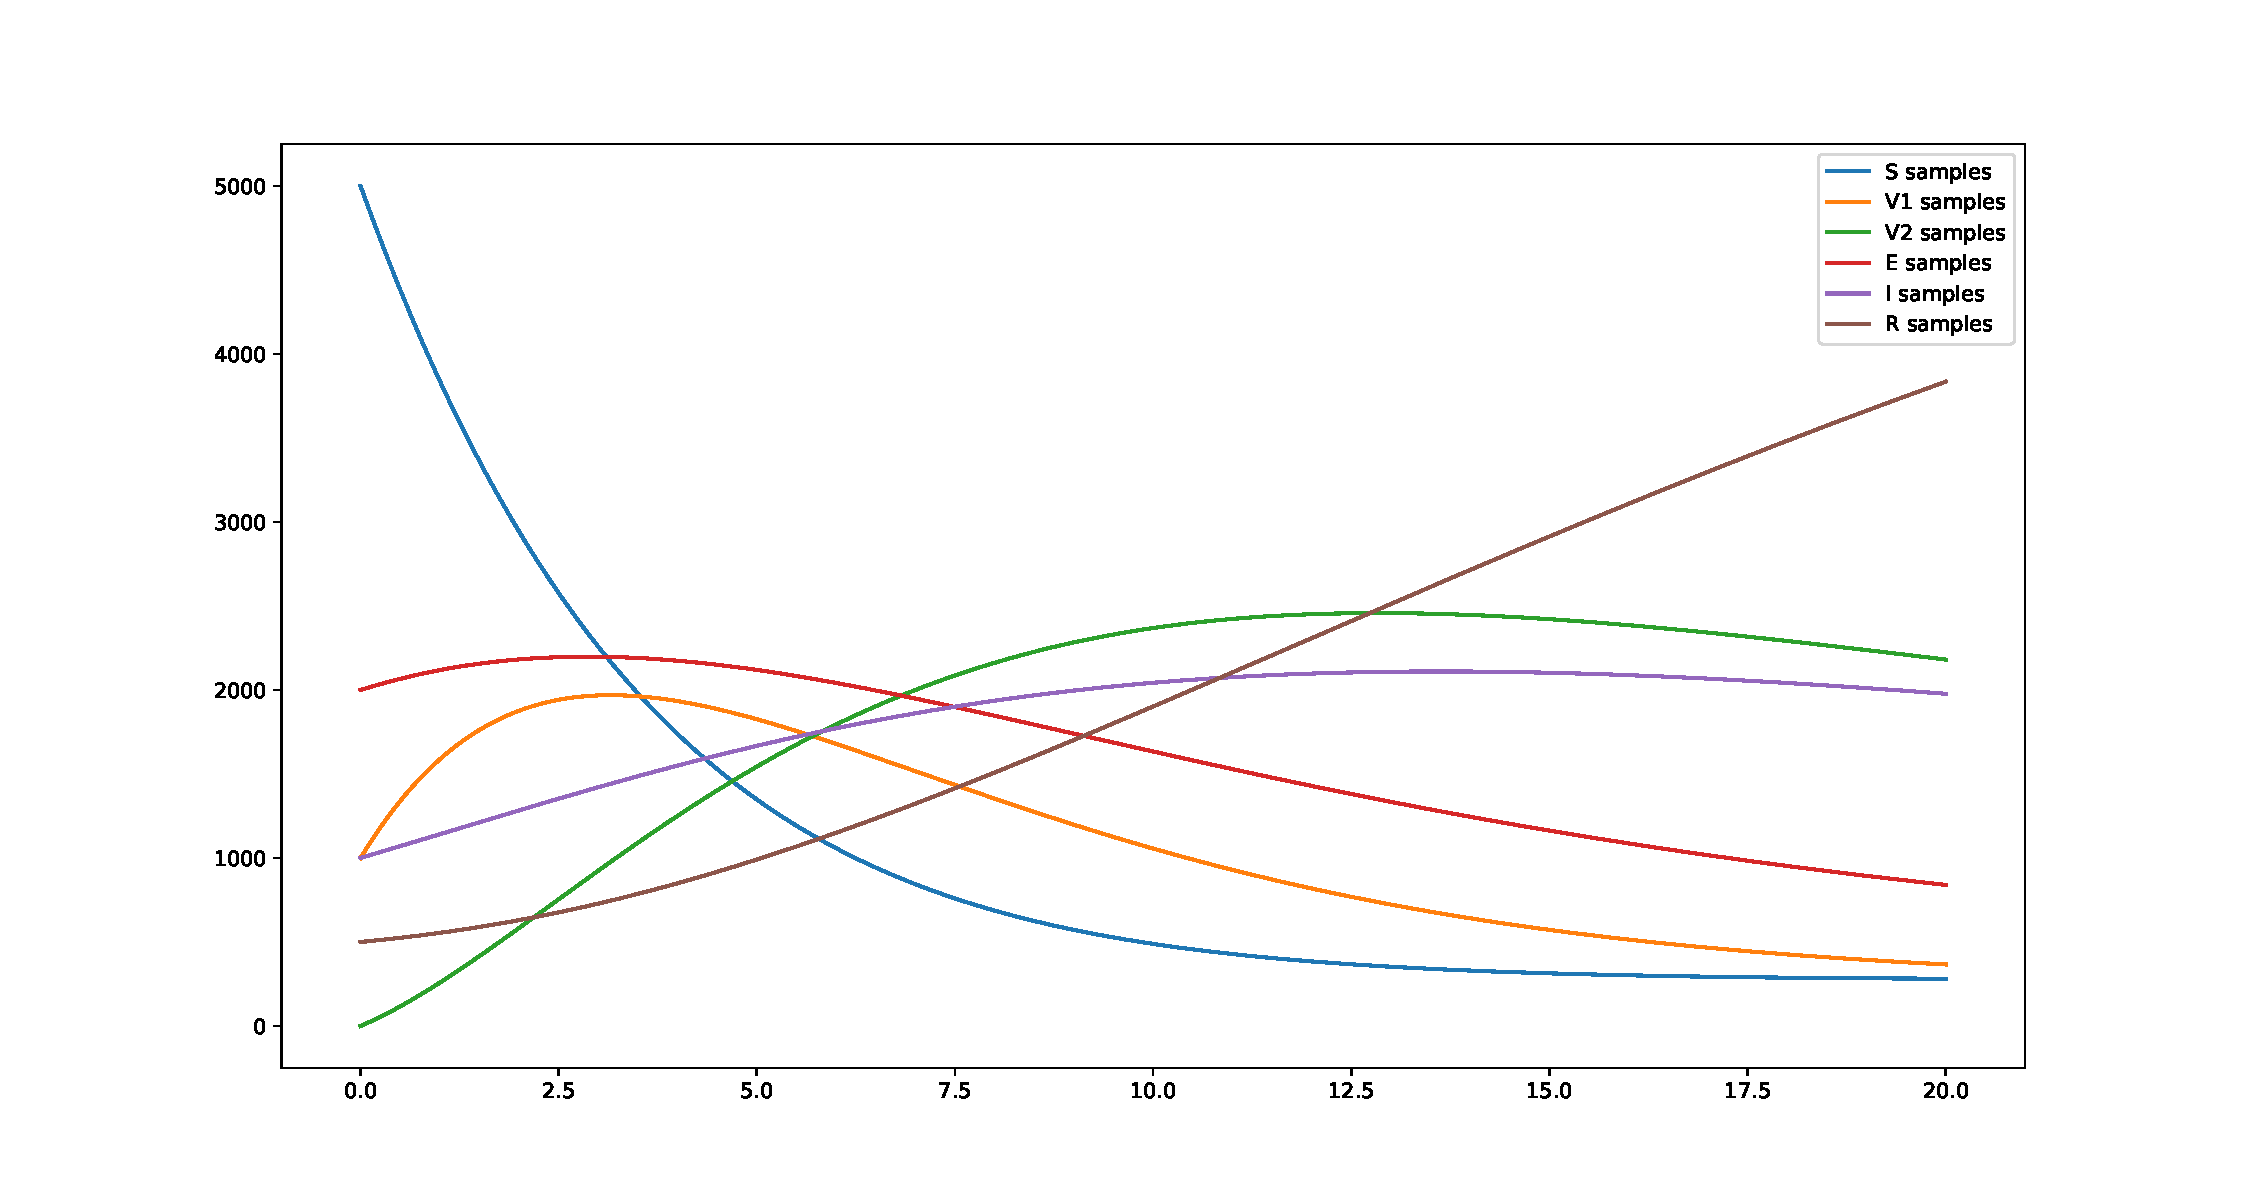
\includegraphics[width=\textwidth]{"figures/SVVEIR.pdf"}
    \caption{modelo SVVEIR con $\alpha = 0.1$, $\beta = 0.7$, $\delta = 0.0005$, $\gamma = 0.05$, $\mu = 0.01$, $n = 0.2$, $\rho = 0.01$, $\omega = 0.05$ y $\sigma = 0.2$.}
    \label{fig:SVVEIR}
\end{figure}

Los resultados que se obtienen durante las 30 ejecuciones del experimento, utilizando solamente en cada ecuación las variables permitidas según el modelo y además se agrega como varible $N=S + V_1 + V_2 + E + I + R$, aparecen en la tabla \ref{table:experiment_SVVEIR} de la página \pageref{table:experiment_SVVEIR}. Si se permite cualquier variable del modelo en cualquier ecuación del sistema se obtienen los datos que aparecen en la tabla \ref{table:experiment_SVVEIR_all} de la página \pageref{table:experiment_SVVEIR_all}.

\begin{table}[!h]
    \centering
    \caption{Resultados que se obtienen en el modelo SVVEIR restringiendo las variables que aparecen en cada ecuación.}
    \begin{tabular}{|c|c|c|c|}
        \hline
               & \textbf{ruido de 0\%} & \textbf{ruido de 5\%} & \textbf{ruido de 10\%} \\
        \hline
        media  & 3.64426               & 13.57802              & 16.12164               \\
        \hline
        mínimo & 1.30096               & 9.50931               & 12.69225               \\
        \hline
        máximo & 14.28797              & 29.02875              & 25.4523                \\
        \hline
    \end{tabular}

    \begin{tabular}{|c|c|c|c|c|c|}
        \hline
                             & \textbf{ruido de 0\%} & \textbf{ruido de 5\%} & \textbf{ruido de 10\%} \\
        \hline
        cantidad de sistemas & 30                    & 30                    & 29                     \\
        \hline
        original             & 26.41261              & 121.61259             & 94.25209               \\
        \hline
        original con ruido   & 26.41261              & 146.93245             & 165.1642               \\
        \hline
        spline               & 26.41261              & 121.72339             & 94.75343               \\
        \hline
        otro método          & 1431.78292            & 1415.93366            & 1612.23507             \\
        \hline
    \end{tabular}
    \label{table:experiment_SVVEIR}
\end{table}

\begin{table}[!h]
    \centering
    \caption{Resultados que se obtienen en el modelo SVVEIR sin restringir las variables que aparecen en cada ecuación.}
    \begin{tabular}{|c|c|c|c|}
        \hline
               & \textbf{ruido de 0\%} & \textbf{ruido de 5\%} & \textbf{ruido de 10\%} \\
        \hline
        media  & 8.30945               & 15.87176              & 17.95833               \\
        \hline
        mínimo & 1.76748               & 10.78393              & 12.29942               \\
        \hline
        máximo & 45.85105              & 47.08811              & 44.09112               \\
        \hline
    \end{tabular}

    \begin{tabular}{|c|c|c|c|c|c|}
        \hline
                             & \textbf{ruido de 0\%} & \textbf{ruido de 5\%} & \textbf{ruido de 10\%} \\
        \hline
        cantidad de sistemas & 30                    & 28                    & 30                     \\
        \hline
        original             & 146.5678              & 215.51733             & 173.10665              \\
        \hline
        original con ruido   & 146.5678              & 234.37447             & 230.006                \\
        \hline
        spline               & 146.5678              & 216.31001             & 172.30783              \\
        \hline
        otro método          & 1433.89796            & 1355.59667            & 1654.19469             \\
        \hline
    \end{tabular}
    \label{table:experiment_SVVEIR_all}
\end{table}

Con este experimento se obtiene que los sistemas generados por la regresión simbólica ajustan los datos mientras estos no posean ruido. Los datos que se obtienen de la integración del sistema resultante de la regresión simbólica se asemejan a los datos de la integración del sistema seleccionado para la realización del experimento pero la aparición de ruido afecta el ajuste de los datos.

En las figuras \ref{fig:final_plot_SVVEIR_0.0} de la página \pageref{fig:final_plot_SVVEIR_0.0}, \ref{fig:final_plot_SVVEIR_0.05} de la página \pageref{fig:final_plot_SVVEIR_0.05} y \ref{fig:final_plot_SVVEIR_0.1} de la página \pageref{fig:final_plot_SVVEIR_0.1} se pueden ver los datos originales comparados con los datos obtenidos del mejor resultado generado por la regresión simbólica restringiendo las variables que pueden existir en cada ecuación.

\begin{figure}[h]
    \centering
    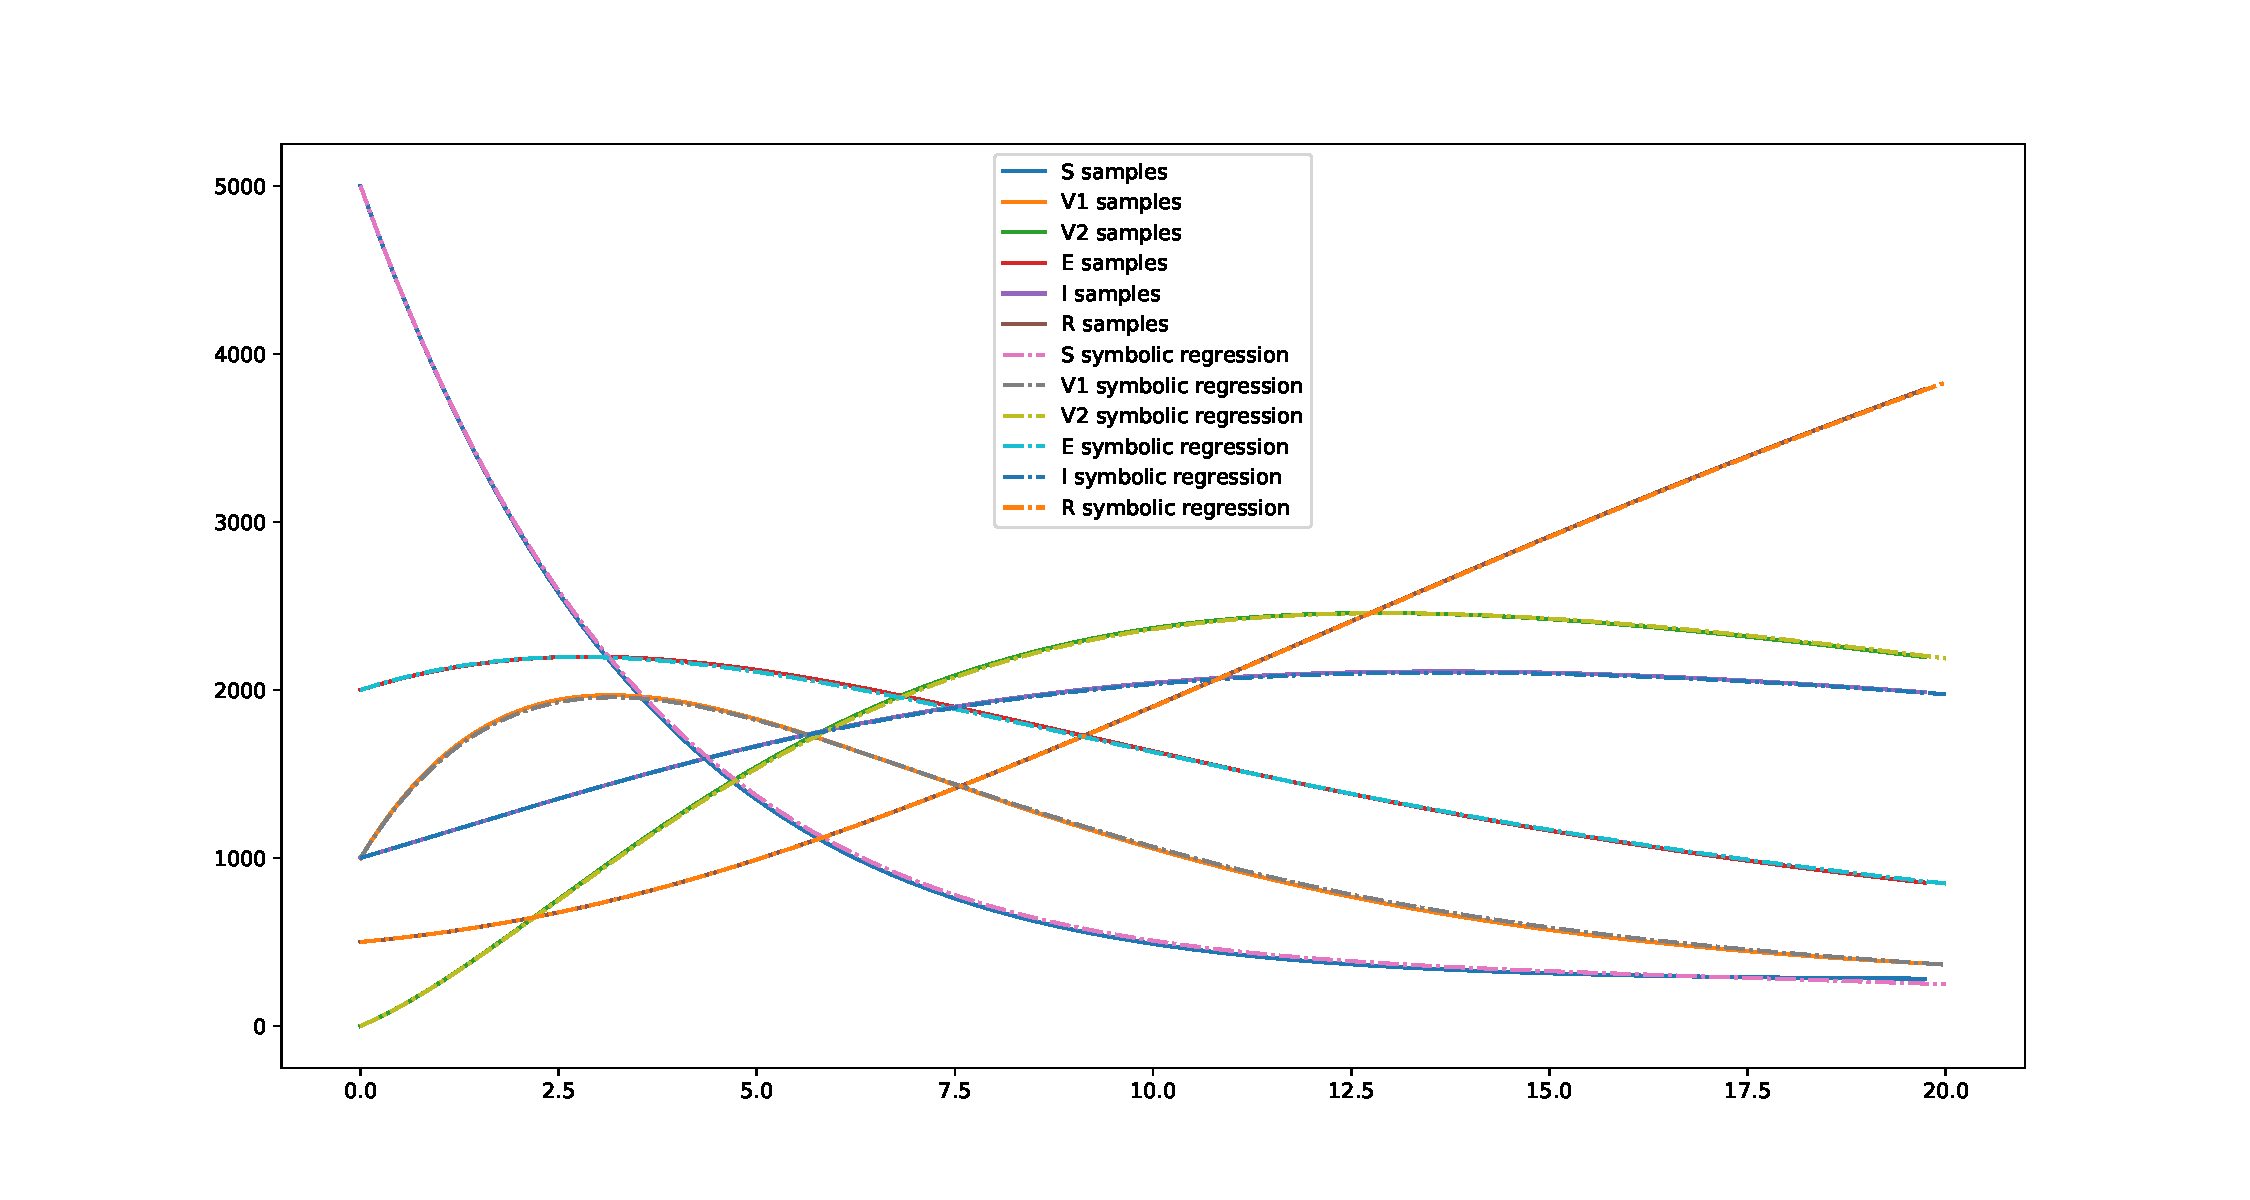
\includegraphics[width=\textwidth]{"figures/final_plot_SVVEIR_0.0.pdf"}
    \caption{Modelo resultante utilizando datos generados a partir del modelo SVVEIR con ruido máximo de 0\%.}
    \label{fig:final_plot_SVVEIR_0.0}
\end{figure}

\begin{figure}[h]
    \centering
    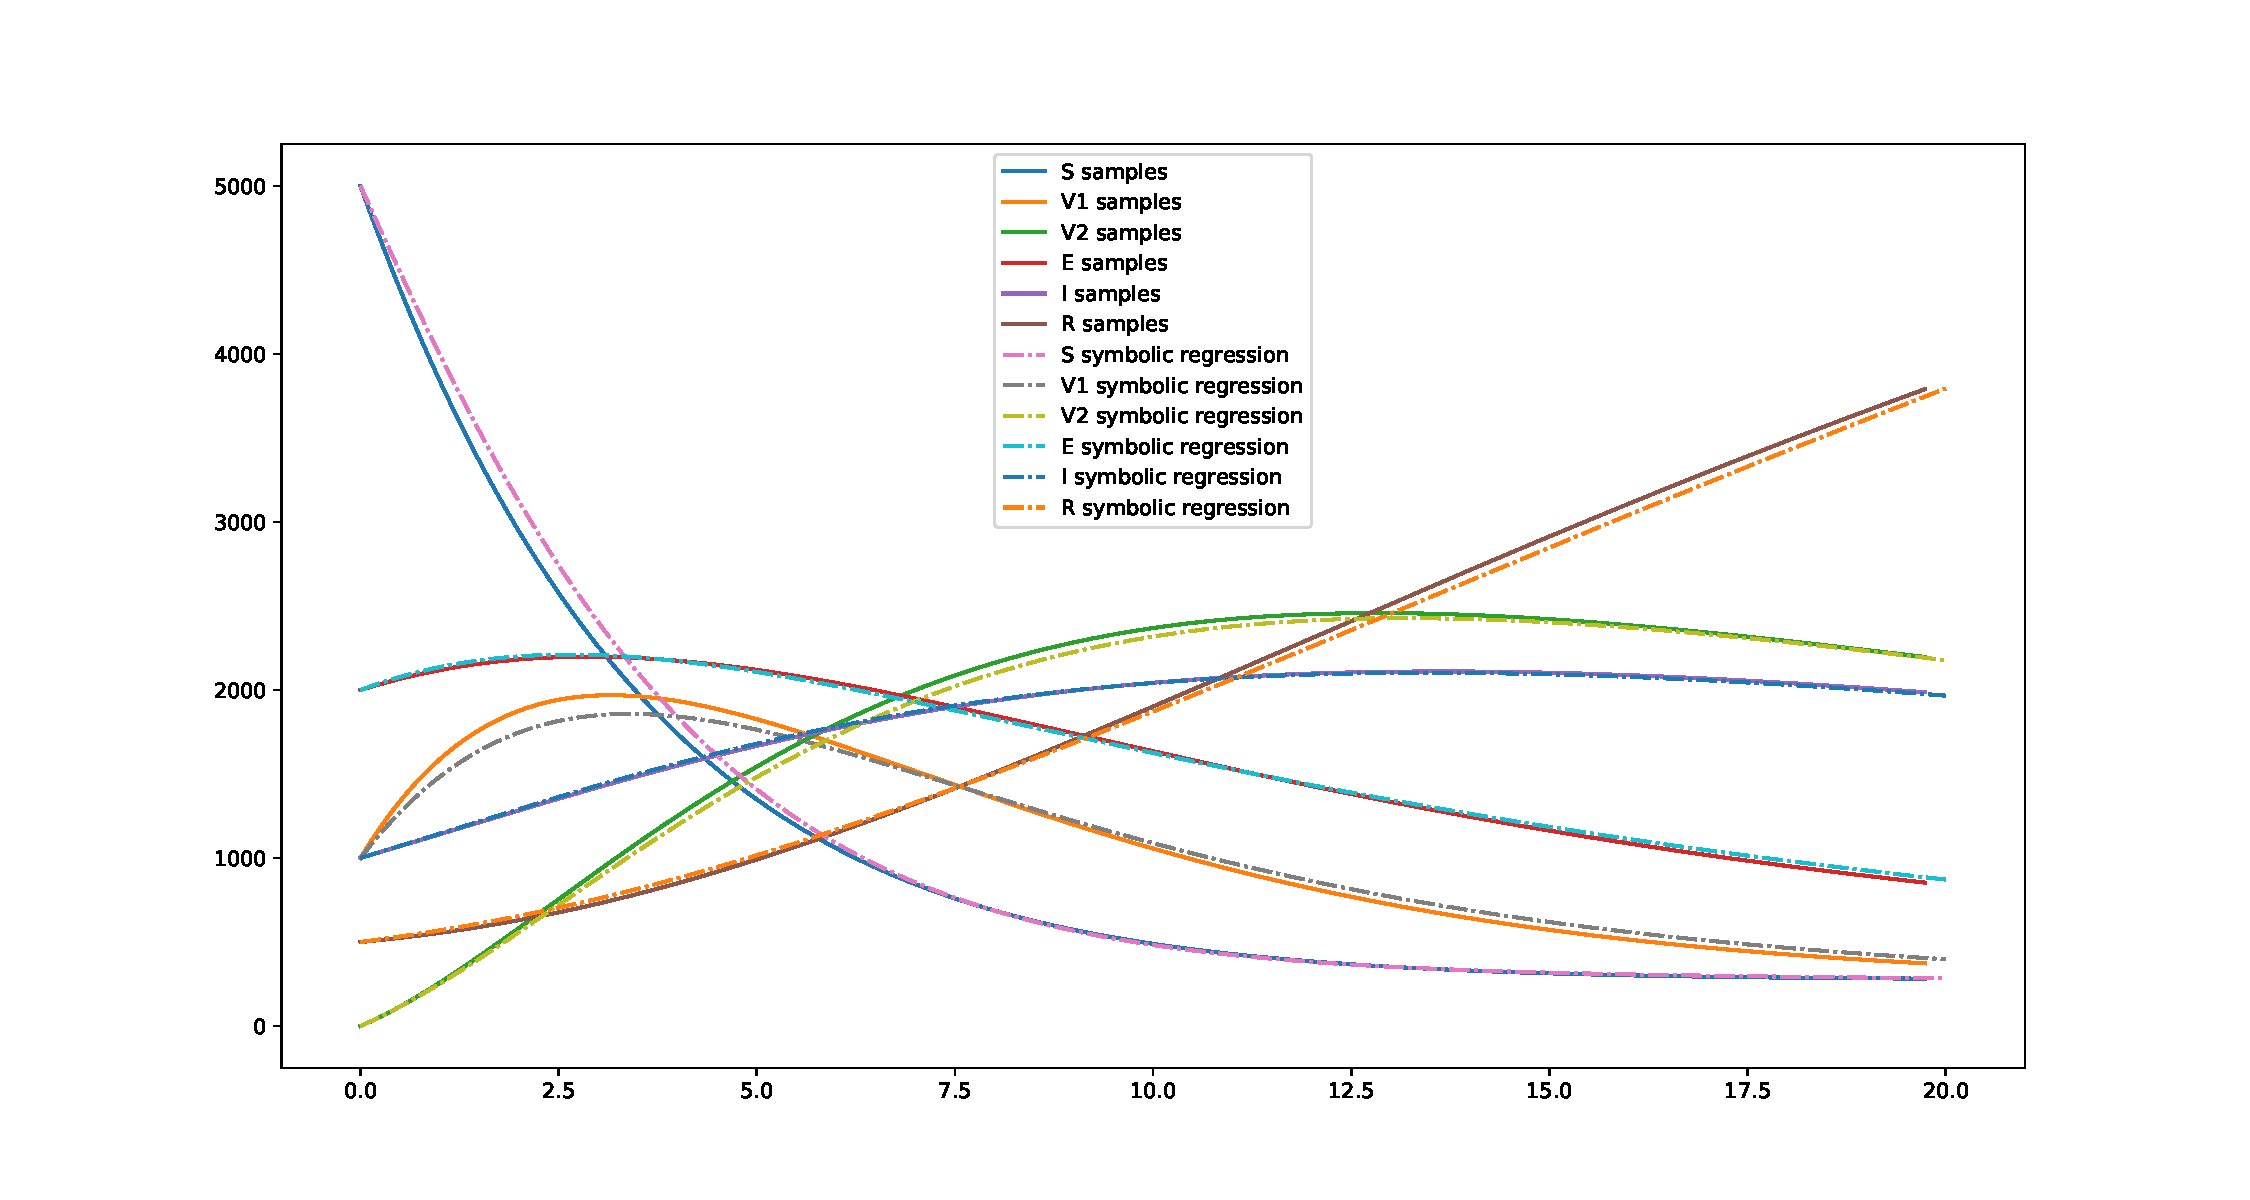
\includegraphics[width=\textwidth]{"figures/final_plot_SVVEIR_0.05.pdf"}
    \caption{Modelo resultante utilizando datos generados a partir del modelo SVVEIR con ruido máximo de 5\%.}
    \label{fig:final_plot_SVVEIR_0.05}
\end{figure}

\begin{figure}[h]
    \centering
    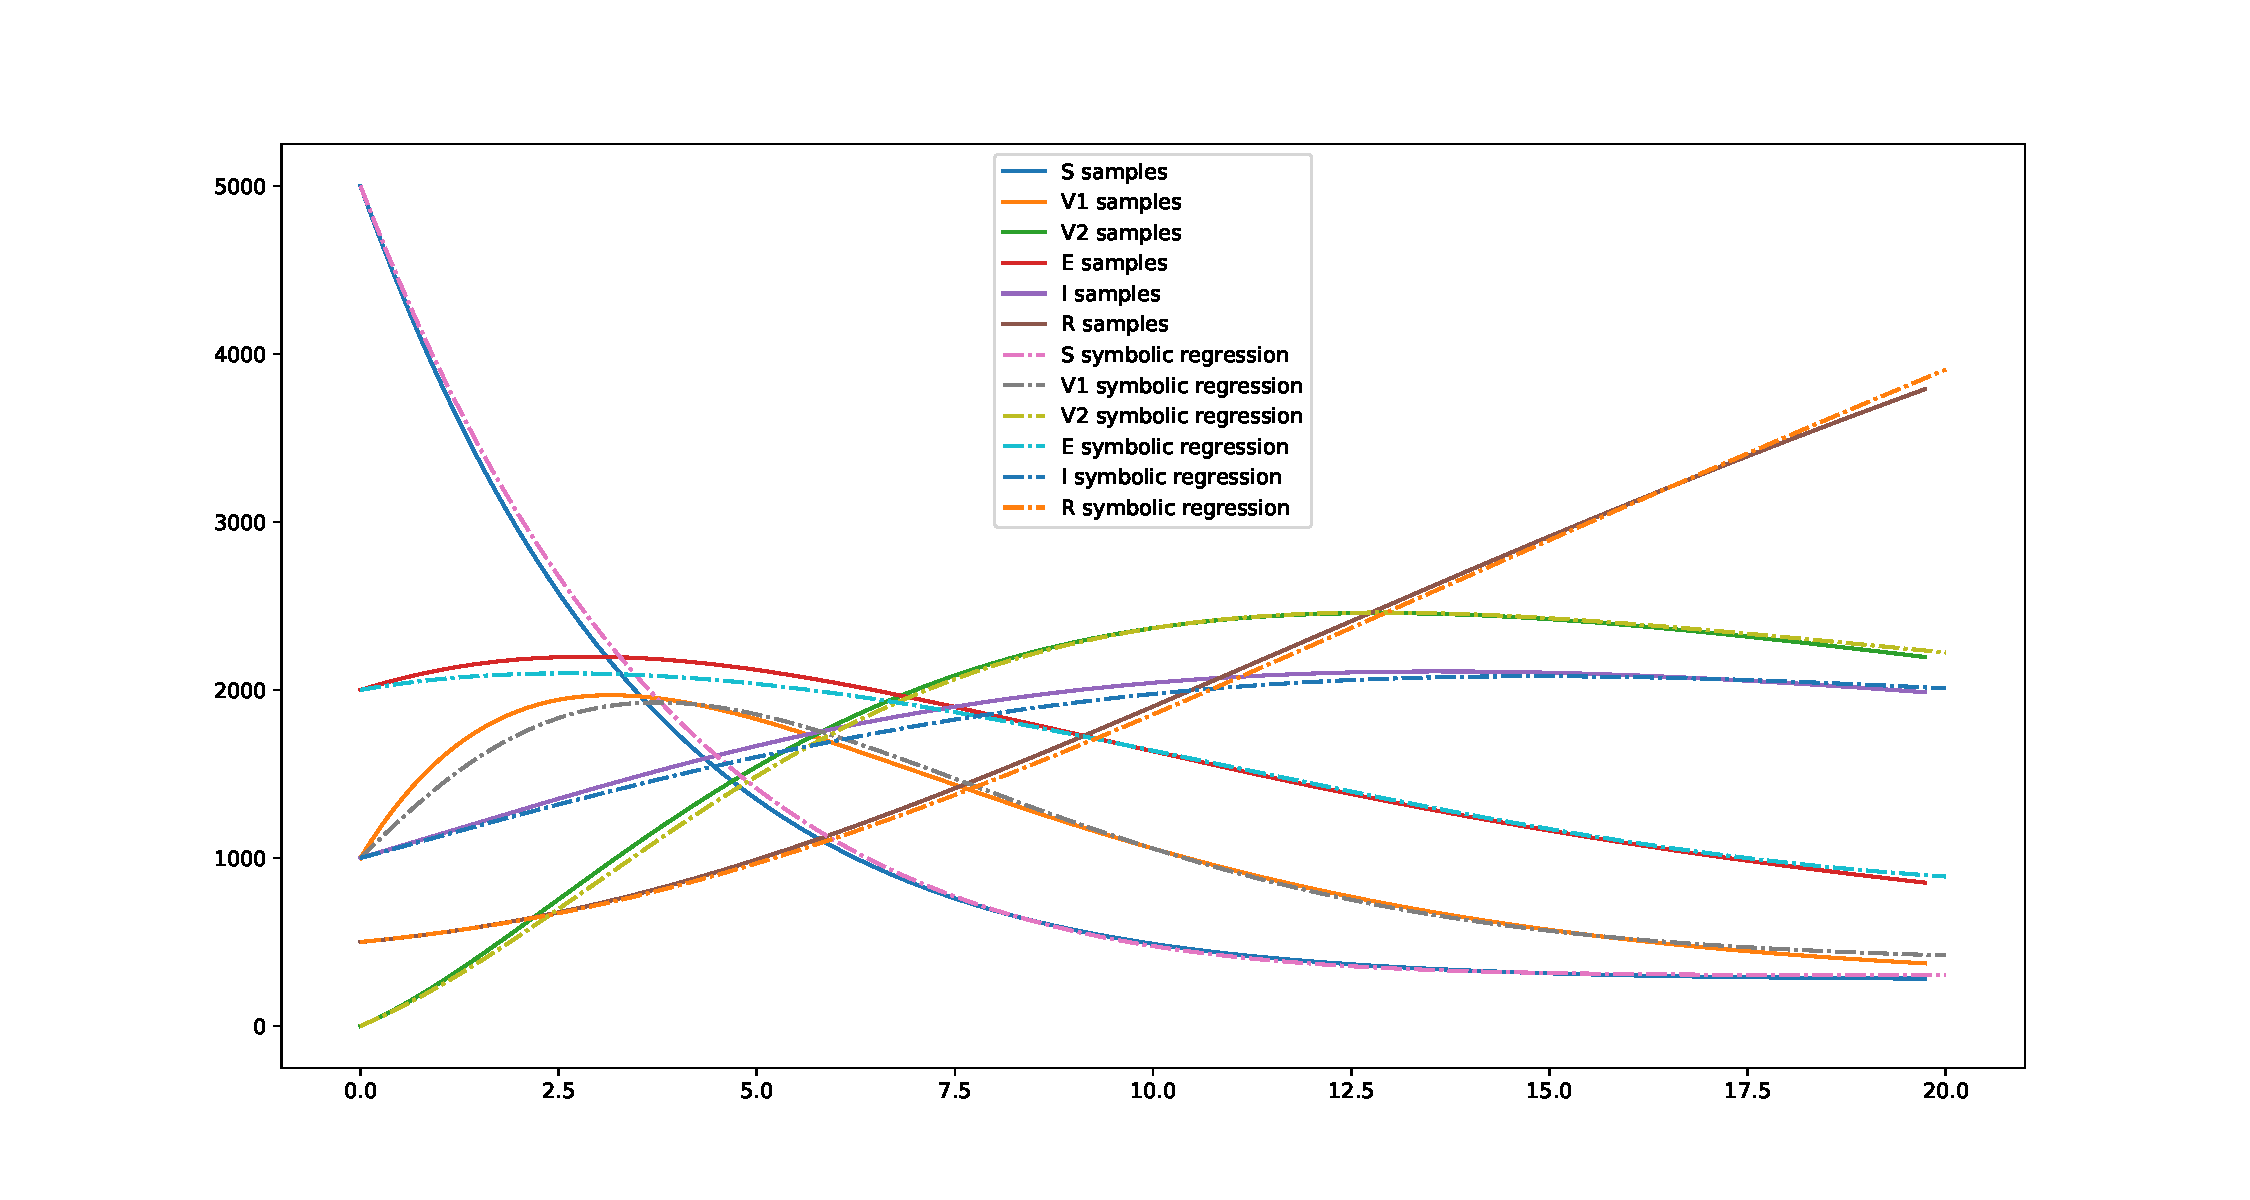
\includegraphics[width=\textwidth]{"figures/final_plot_SVVEIR_0.1.pdf"}
    \caption{Modelo resultante utilizando datos generados a partir del modelo SVVEIR con ruido máximo de 10\%.}
    \label{fig:final_plot_SVVEIR_0.1}
\end{figure}

Si en lugar de utilizar como aproximación el método de diferencias finitas cuando los datos no poseen ruido, se utiliza el sistema original de SIR, se obtiene que la media del valor de la función de ajuste a lo largo de las 30 ejecuciones del experimento es $3.68731$. El valor máximo de la función de ajuste alcanzado fue de $19.45527$ y el mínimo de $0.58707$, en este último la regresión simbólica no obtuvo el sistema original.

En la siguiente sección se realiza un análisis de los resultados de todos los experimentos realizado.

\section{Análisis de resultados}\label{section:experiments_results}

Los resultados obtenidos durante los experimentos muestran que la regresión simbólica planteada puede encontrar un sistema $f_{aprox}$ que ajuste los datos $y'_{original}$ generados a partir de la derivada aproximada por el método de diferencias finitas sobre los datos $y_{original}$ donde $y_{original}$ son los datos obtenidos de la integración del sistema conocido $f$.

Al generar el conjunto $y_{noise}$ a partir de agregar ruido a $y_{original}$ que describen la función $y$, no se puede aproximar la derivada de $y$ por el método de diferencias finitas. La función $y$ se aproxima utilizando un spline de suavizado cúbico sobre $y_{noise}$ obteniéndose los datos $y_{spline}$. Del spline de suavizado se puede obtener el valor de la primera derivada y así generar el conjunto $y'_{spline}$. Al utilizar los valores de $y_{spline}$ y $y'_{spline}$ en el método de regresión simbólica se obtiene el sistema $f_{aprox_{sr}}$.

El error cuádratico médio de los datos $y_{spline}$ evaluados en el sistema $f_{aprox_{sr}}$ es mayor que el de los datos $y_{original}$ evaluados en el sistema $f_{aprox}$. Mientras mayor el ruido presente en $y_{noise}$ mayor es la diferencia entre los valore del ajuste.

Si se integra el sistema $f_{aprox}$ se obtiene el conjunto de puntos $y_{aprox}$. El valor del error cuádratico medio entre los conjuntos $y_{aprox}$ y $y_{original}$ es menor en los sistemas que no poseen términos con un parámetro sin estar multiplicando una expresión.

Si se definen los datos $y_{aprox_{sr}}$ como el resultado de la integración del sistema $f_{aprox_{sr}}$, se puede analizar como el error cuadrático medio entre los puntos $y_{aprox_{sr}}$ y $y_{spline}$ es igual que el error cuádratico medio entre los puntos $y_{aprox_{sr}}$ y $y_{original}$.

En los sistemas con menos de 6 ecuaciones, los resultados de aplicar la restricción de las variables que pueden existir en cada ecuación son semejantes a los resultados obtenidos sin aplicar la restricción.

En los experimentos utilizando los modelos SIR, SIRD, SIQRD y SVVEIR nunca se obtuvo el sistema original como resultado de la regresión simbólica, sin embargo si se obtuvieron sistemas que fueron capaces de ajustar los datos con valores en la función de ajuste cercanos a 0.

La utilización del modelo original para la aproximación de $y'_{original}$ hace que se obtengan los resultados con el menor valor de ajuste, obtiéndose exactamente el sistema original en algunos experimentos correspondientes a los modelos Lotka-Volterra, SIR, SIRD y SIQRD.

\backmatter

\chapter*{Conclusiones}\label{chapter:conclusions}
\addcontentsline{toc}{chapter}{Conclusiones}

En este trabajo se diseño e implementó un sistema de regresión simbólica basada en algoritmos genéticos para encontrar un sistema de ecuaciones diferenciales lineales con respecto a los parámetros en el que es posible determinar qué variables intervienen en cada ecuación.

Con este fin se definió cómo representar los sistemas de ecuaciones diferenciales en forma de árbol computacional de manera que solo se permitiese representar sistemas lineales con respecto a los parámetros. Para el uso del algoritmo genético se definieron las operaciones de mutación, cruzamiento y selección sobre estos árboles. Además se utilizó un spline de suavizado para eliminar el ruido en los datos.

Se utilizó la propiedad de linealidad con respecto a los parámetros de los sistemas de ecuaciones para ajustar los parámetros en cada solución resolviendo un sistema de ecuaciones lineales.

Para probar el funcionamiento del sistema creado se utilizaron datos generados a partir de 5 sistemas de ecucaciones diferenciales conocidos, comprobándose así la calidad de las soluciones obtenidas por la regresión simbólica.
\begin{recomendations}

    Los parámetros utilizados en el algoritmo genético empleado en la regresión simbólica fueron los mismos en cada experimento, se recomienda hacer un estudio de la selección de estos parámetros.

    Para impedir que árboles con más de $k$ niveles se puedan obtener, se propone modificar las operaciones de mutación y cruzamiento, siendo $k$ otro parámetro que se puede incorporar al algoritmo genético.

    Como trabajo futuro se puede estudiar la cantidad de muestras sin ruido mínimas necesarias para obtener exactamente el sistema que originó los datos.

    Buscar formas de lidiar con los sistemas con grandes expresiones, como la división presente en la primera y segunda ecuación del sistema SIRD.

\end{recomendations}

\nocite{*}
\bibliographystyle{plain}
\bibliography{Bibliography}
\end{document}